\documentclass[
	fontsize=10pt, 
	twoside=true, 
	numbers=noenddot, 
]{kaobook}
\usepackage{blindtext}
\usepackage{styles/kaobiblio}
\addbibresource{main.bib}
\usepackage{styles/mdftheorems}
\usepackage{amssymb,amsmath,stmaryrd}
\usepackage[italian]{babel}
\usepackage{pdfpages}

\makeindex[columns=2, title=Indice Alfabetico, intoc]

\usepackage[utf8]{inputenc}

\newcommand{\mathtext}[1]{\mbox{$\mathrm{#1}$}}
\newcommand{\mathtextbold}[1]{\mbox{$\boldsymbol{\mathrm{#1}}$}}

\graphicspath{{images/}}
\begin{document}
\includepdf{images/copertina.jpg}

\title[Appunti di metallurgia]{Appunti di metallurgia}
\subtitle{per il corso del prof. Scavino}
\author[Enrico Foglia, IL Mara]{IL Mara\thanks{Un pazzo che aveva un sacco di tempo libero, a cui tutti noi dobbiamo la nostra libertà.}, Enrico Foglia\thanks{Non aveva un cazzo da fare}}\footnote[0]{Copertina: @scottweb su unsplash.com}
\date{}

\frontmatter

\makeatletter
\lowertitleback{
\textbf{Disclaimer}\\
Gli appunti che seguono sono i leggendari appunti del Mara, rivisti e riproposti in una veste grafica più carina da Enrico Foglia.\\
Il corso di Scavino, si sa, è un giungla con tanto di vietcong, dunque si spera che negli anni questa raccolta di sapere possa essere ampliata e migliorata fino alla perfezione. I margini larghi sono pensati apposta per poter contenere di anno in anno le novità del nostro professore preferito. Usate questi appunti senza ritegno, scarabocchiate, spotacciate e migliorate tutto quello che vi sentite. Solo: non vendeteli. Sono pensati come strumento per superare insieme un momento difficile, quindi non fate gli stronzi.
}
\makeatother


\KOMAoptions{twoside=semi}
\maketitle
\KOMAoptions{twoside=false}

\begingroup % Local scope for the following commands

% Define the style for the TOC, LOF, and LOT
%\setstretch{1} % Uncomment to modify line spacing in the ToC
%\hypersetup{linkcolor=blue} % Uncomment to set the colour of links in the ToC
\setlength{\textheight}{23cm} % Manually adjust the height of the ToC pages

% Turn on compatibility mode for the etoc package
\etocstandarddisplaystyle % "toc display" as if etoc was not loaded
\etocstandardlines % toc lines as if etoc was not loaded

\tableofcontents % Output the table of contents

\endgroup


\mainmatter
\setchapterstyle{kao}


\setchapterpreamble[u]{\margintoc}
\chapter{Cos'è un materiale metallico?}
\labch{cap1}
\index{metallurgia}
La metallurgia è la scienza e la tecnologia dei materiali metallici.
I materiali metallici si distinguono in:
\begin{itemize}
    \item \textbf{metalli puri}, rarissimi e di nessuna utilità, poiché hanno delle caratteristiche meccaniche bassissimi e scarse applicazioni;
    \item \textbf{leghe}, sono materiali con caratteristiche metalliche formati da più componenti, cioè da più metalli (es bronzo) o un metallo e da un non metallo (es acciaio), detto metalloide.
    \index{acciaio} \index{ghisa}
L’acciaio è la ferrolega più comune, formata da ferro e carbonio e in parti minori da manganese e silicio, già presenti nel minerale. Fino al 2\% di carbonio questa lega viene definita acciaio, al di sopra di tale valore si parlerà invece di ghisa. Tuttavia, aggiungendo altri elementi, si possono ottenere acciaio con tenori di carbonio superiori al 2\% e ghise con tenori di carbonio minori del 2\%. Nel campo aerospaziale, sono molto diffuse le leghe di alluminio, sia con metalli sia con non metalli (ex. lega di alluminio e silicio).
Non sempre l’unione di un metallo e di un non metallo dà origine a una lega, ma dipende dalle caratteristiche del prodotto finale, cioè da come si comporta tale materiale. Distinguiamo, infatti, le leghe dagli ossidi, materiali formati dall’unione di ossigeno O e di un metallo. Ad esempio, il ferro forma anche degli ossidi, come l’ematite $\mathrm{Fe_2O_3}$, la magnetite $\mathrm{Fe_3O_4}$ e la wustite $\mathrm{FeO}$. Altri ossidi importanti sono l’allumina $\mathrm{Al_2O_3}$, l’ossido di titanio $\mathrm{TiO_2}$ e l’ossido di calcio, o calce viva, $\mathrm{CaO}$.
Essi non possono essere considerati materiali metallici, in quanto privi delle caratteristiche che rendono tale un materiale metallico. Infatti, i materiali metallici hanno caratteristiche specifiche.
\end{itemize}
\setchapterpreamble[u]{\margintoc}
\chapter{Caratteristiche dei materiali metallici}
\labch{cap2}

\section{Introduzione}
Le caratteristiche di un materiale dipendono dalla composizione chimica e dal trattamento termico
che hanno subito.
Le caratteristiche che citeremo sono delle caratteristiche esclusive dei materiali metallici, ma esse non sono le uniche in quanto i metalli condividono importanti proprietà con le altre famiglie di materiali. Tra le caratteristiche comuni vi è la rigidezza (anche la pietra è rigida), lo stato solido (anche il ghiaccio è solido) e la struttura cristallina, che prevede una disposizione geometrica definita degli atomi che si ripete nello spazio (ordine a lungo raggio).

Possiamo distinguere diverse proprietà che rendono i materiali metallici i più impiegati nel settore aeronautico e, in generale, in campo industriale:

\index{lucentezza}
\begin{itemize} 
    \item \textbf{Lucentezza}: in opportune condizioni i materiali metallici sono degli specchi. Questa caratteristica è stata la prima ad essere sfruttata dall’uomo: la prima applicazione dei materiali metallici è stata lo specchio in rame e la creazione di monili. Infatti, sideros, dal greco, significa oggetto che brilla. Paradossalmente, un metallo in genere non riflette la luce perché la sua superficie è ricoperta da materiale non metallico, per evitare la corrosione. Infatti, i metalli reagiscono a contatto con l’ossigeno e si ossidano, dando vita a fenomeni di ruggine. Ad esempio, l’acciaio inossidabile presenta uno strato di ossido protettivo. La lucentezza si ha quando il materiale metallico ha una superficie piana e metallica, cioè non ossidata, in quanto l’ossido non è un materiale metallico e non riflette la luce, come tutti i materiali non metallici in generale. L’ossidazione è un processo naturale e il procedimento utilizzato per rimuovere lo strato ossidato è molto costoso, quindi per riflettere si preferisce l’uso di altri materiali. La lucentezza viene, inoltre, usata per studiare la struttura dei materiali;
    \item \textbf{Conducibilità elettrica}\index{conducibilità elettrica}:i materiali metallici sono ottimi conduttori elettrici. Essi sono caratterizzati da una conducibilità di tipo ionico, tipica anche dei non metalli, e da una conducibilità di tipo elettronico, tipica dei materiali metallici. Quest’ultima è resa possibile dalla presenza del legame metallico;
    \item\textbf{Conducibilità termica}\index{conducibilità termica}: materiali metallici sono ottimi conduttori di calore grazie alla presenza di elettroni liberi di muoversi (agitazione termica), caratteristica tipica del legame metallico. Le due conducibilità sono caratteristiche molto utilizzate a livello tecnologico;
    \item \textbf{Comportamento elettrochimico}\index{comportamento elettrochimico}: i metalli si elettrizzano positivamente;
    \item \textbf{Proprietà magnetiche};
    \item \textbf{Riciclabilità}\index{riciclabilità}: non è una proprietà esclusiva dei materiali metallici (anche i vetri sono riciclabili);
    \item \textbf{Deformabilità plastica}\index{deformabilità plastica}:è la caratteristica principale dei materiali metallici. Si tratta della capacità di subire grandi cambiamenti irreversibili di forma in risposta a forze applicate e conseguente assorbimento di energia. Comporta la possibilità di produrre dei componenti meccanici sicuri, poiché non si rompono facilmente, ed è utilissima non solo nella produzione, ma soprattutto nell’impiego di tali parti. Il materiale metallico, infatti, se sollecitato fortemente si deforma prima elasticamente, come tutti i materiali, e poi anche plasticamente: ciò permette di usare tale materiale in sicurezza, poiché presenta carichi critici molto elevati, cosa che invece non accade negli altri materiali, dove si assiste a fenomeni di rottura per carichi molto inferiori. In particolare, la deformabilità può essere controllata attraverso dei meccanismi di rafforzamento, quali i trattamenti termici (trattamento superficiale). Tra le lavorazione a deformazione plastica ricordiamo la laminazione, la trafilatura e la calandratura. Dopo aver realizzato un materiale per deformazione plastica (produzione), bisogna effettuare un controllo della deformabilità, con successivi interventi di rafforzamento (trattamenti termici) e il successivo studio dei fenomeni di rottura.
    \item \textbf{Colabilità}\index{colabilità}:è l'attitudine di un materiale a riempire completamente un contenitore di qualsiasi forma una volta allo stato liquido. Le ghise hanno un’elevata colabilità e possono essere gettate in stampi con forma pressoché definitiva.

\end{itemize}

Tuttavia, bisogna trovare il giusto compromesso fra tutte queste caratteristiche. Ad esempio, se un materiale è troppo deformabile, non è abbastanza resistente. Un miglioramento si ha, ad esempio, con i meccanismi di rafforzamento, che riducono la deformabilità pratica e permettono di operare in maggiore sicurezza.

\section{Conducibilità elettrica}\label{PropElettriche} \index{conducibilità elettrica}

Tutte le sostanze che contengono ioni sono buoni conduttori di corrente, come ad esempio l'acqua. Inoltre, quando nell'acqua sono presenti altre sostanze, esse subiscono il fenomeno dell'elettrolisi e si dissociano in ioni.

I metalli sono degli ottimi conduttori; come detto nel paragrafo precedente, i materiali metallici oltre la conduzione di tipo ionico conducono anche in modo elettronico, grazie al loro caratteristico legame metallico(il quale ha il pregio di unire le caratteristiche del legame ionico a quelle del legame covalente).
Gli elettroni possiedono una certa energia e, nella struttura atomica, si posizionano in zone a loro energicamente concesse (che prendono il nome di orbitali). Queste zone sono definite come quelle in cui la probabilità di trovare l'elettrone è più alta. 
\newline \index{legame metallico}
Nel legame metallico, però, gli elettroni più esterni possono allontanarsi dal nucleo, formando u a nube elettronica mobile, detta mare di Fermi, sensibile ai campi elettrici, determinando in tal modo anche le proprietà magnetiche dei metalli.
Siccome solo gli elettroni degli orbitali più esterni hanno la possibilità di staccarsi dal nucleo, si definisce \textbf{banda di conduzione} la banda elettronica a più bassa energia tra quelle non completamente occupate.

\begin{figure}[!hbt]
	\includegraphics[width=0.6\textwidth]{images/img1.png}
	\caption[Banda di valenza]{separazione dei livelli energetici in metalli, semiconduttori e metalli}
	\labfig{img1}
\end{figure}

Tale banda, nei metalli, è parzialmente riempita e restano degli spazi vacanti \sidenote{Alla banda 's' sono legate le proprietà elettriche, alla banda 'p' quelle magnetiche}: gli elettroni che vi appartengono hanno la possibilità di spostarsi in livelli energetici diversi, divisi da un salto energetico infinitesimale, e hanno quindi un'elevata mobilità che determina l'alta conducibilità elettrica del materiale.

I metalli possono avere dei difetti reticolari puntiformi consistenti nella mancanza di un atomo nel reticolo (\textbf{vacanza} o gap) o nella presenza di un atomo estraneo (\textbf{impurità}): questi possono rappresentare dei vantaggi come degli svantaggi. Nel caso specifico della conduzione elettrica, le vacanze rappresentano degli ostacoli al passaggio di elettroni ed aumentano quindi la resistività del materiale. Il numero di vacanze è legato esponenzialmente alla temperatura: \index{vacanza}
\begin{equation*}
    \frac{\mathrm{n_{vacanze}}}{\mathrm{n_{ atomi}+n_{vacanze}}} = e^{-Q/RT}
\end{equation*}

Dove Q è il cosiddetto calore di attivazione, ovvero la quantità di energia necessaria a generare una mole di vacanze.\\

I conduttori elettrici sono fatti perlopiù di \textbf{rame}, poiché rappresentano il giusto compromesso tra conducibilità elettrica, caratteristiche meccaniche e costi\sidenote{Il rame è stato il primo metallo tecnologicamente impiegato dall'uomo (5000-6000 a.C.) perché facilmente reperibile e lavorabile. Venne poi soppiantato dal \textbf{bronzo} una lega metallica di rame e stagno, rame alluminio (bronzi all'alluminio), rame e zinco (ottoni). Solo nel 1200 a.C. si cominciò ad impiegare il \textbf{ferro}.}. \newline
Per permettere il passaggio di elettroni il metallo dev'essere il più puro possibile e con il minor numero possibile di vacanze. Il rame puro è molto costoso e difficile da realizzare. Non stupisce quindi che quello che poteva essere ottenuto nei secoli scorsi dalla fusione dei minerali era altamente impuro e quindi con una conducibilità elettrica limitata. \newline
Per ottenere rame puro si parte da quello impuro e, tramite diverse tecniche, si procede con la raffinazione.

La prima tecnica è \textbf{la fusione a zone}, che si basa sul presupposto di mettere a contatto un solido e un liquido al fine di concentrare le impurità nella fase liquida. Per comprendere questa tecnica analizziamo un diagramma di stato binario con eutettico: le curve delimitano il campo di esistenza dello stato solido e di quello liquido.
\begin{figure}[!hbt]
	\includegraphics[width=0.6\textwidth]{images/img2.png}
	\caption[Diagramma di stato binario con eutettico]{Diagramma di stato binario con eutettico, relativo a componenti immiscibili allo stato solido e completamente miscibili allo stato liquido}
	\labfig{img2}
\end{figure}
Denotiamo con $\mathrm{T_A}$ e $\mathrm{T_B}$ le temperature di fusione di un generico solido A e B rispettivamente. Rappresentano l'origine delle curve. La curva a T costante che intercetta il punto E, detto \textbf{punto eutettico}, dove si incontrano le curve di fusione di A e B, delimita il campo di coesistenza dei due stati solidi contemporaneamente. \newline
In ascissa è riportata la composizione percentuale della miscela.\newline
Si immagini di avere un materiale solido con una percentuale $\mathrm{C_1}$ di impurità (B) e con il componente A (che supporremo sia rame) molto vicino alla purezza. Aumentando la temperatura oltre il punto di eutettico è possibile notare come la fase liquida formata contenga una concentrazione di B maggiore rispetto a quella di partenza (punto 2), mentre la fase solida resti di A puro (punto 1). Rimuovendo la fase liquida si resta, quindi, con un materiale solido puro.

La fusione può essere effettuata attraverso lo \textbf{scaldamento per induzione}: utilizzando un induttore si riscalda una porzione ristretta del materiale da cui si vogliono eliminare le impurità. In questo modo queste andranno a concentrarsi nella zona fusa del materiale e verranno trascinate dell'induttore stesso fino all'estremità del pezzo. Alla fine del processo la parte terminale dove sono concentrate tutte le impurezze viene rimossa. L'operazione può essere ripetuta più volte fino ad ottenere il livello richiesto di purezza.
\begin{marginfigure}[-5.5cm]
	\includegraphics{images/img3.jpg}
	\caption[Fusione per induzione]{Fusione per induzione.}
	\labfig{img3}
\end{marginfigure}

Non è purtroppo possibile ottenere un materiale puro tramite questo processo: l'operazione successiva è l'\textbf{elettrolisi}. Fondendo il rame non puro ed effettuando l'elettrolisi, al catodo si depositerà il rame puro.

Questo processo di purificazione è utilizzato anche per altri materiali, quali l'\textbf{alluminio} e il \textbf{titanio}. Questi sono molto diffusi sulla crosta terrestre, ma le loro leghe sono estremamente costose da ottenere a causa delle lavorazioni necessarie per ottenerle e per renderle pure (si pensi ad esempio alle temperature necessarie per l'estrazione e l'elettrolisi), a differenza degli acciai e delle ghise che sono ottenuti con processi molto più economici. Gli acciai hanno un prezzo nell'ordine di 1€/kg, l'alluminio di 5-10€/kg e il titanio di 50-100€/kg.

Il rame puro, oltre ad avere un costo commerciale altissimo, presenta delle caratteristiche meccaniche limitate. Queste devono essere quindi migliorate con ulteriori lavorazioni o con l'introduzione di altri elementi chimici, incidendo sulle caratteristiche elettriche del materiale. \newline
Un metodo spesso impiegato in questo senso è l'\textbf{incrudimento}, un processo metallurgico in cui un materiale metallico risulta rafforzato in seguito ad una deformazione plastica a freddo (es. trafilatura o estrusione). Questo incide in primo luogo sulle caratteristiche meccaniche: aumentano limite elastico, carico di rottura e durezza, diminuiscono allungamento, strizione e resilienza. La resistività elettrica subisce un incremento e diminuisce la resistenza alla corrosione. Per questo motivo, nell'indicare in particolare tipo di rame, è necessario indicare anche il grado di incrudimento.

Il rame, sotto alcuni punti di vista, può essere considerato un inquinante, in particolare nei processi di produzione. \\
Per i materiali metallici, in particolare quelli ferrosi, esitono due tipi di processi di produzione: il primo, detto \textbf{integrale}, prevede la produzione del materiala a partire dal minerale; il secondo metodo sfrutta la \textbf{riciclabilità}, fondendo i rottami per poterne usare nuovamente il materiale. Le automobili, ad esempio, vengono costruite con materiali metallici per rispettare l'obbligo del 90-95\% di riciclabilità \sidenote{In tal senso, i materiali devono essere riciclabili non a fini energetici: spesso la riciclabilità viene utilizzata anche nell’accezione di riutilizzabilità, cioè riutilizzo del materiale stesso per produrre altri oggetti.}. I vetri e le lamiere sono riciclabili, mentre la plastica, le gomme le imbottiture dei sedili, i tessuti, etc spesso non lo sono. \\
Nel processo di rottamazione di un'automobile, l'acciaio del telaio può essere inquinato da altri composti: parti di rame, come l'impianto elettrico, e in piombo, come la batteria, possono minare la purezza dell'acciaio. Per ovviare a tale problema, durante il processo di fusione il ferro ottenuto dal rottame viene diluito con dell'acciaio "vergine" (puro) proveniente dagli scarti delle acciaierie primarie per diminuire la concentrazione dei materiali inquinanti.

Nell'ambito della conduzione elettrica, oltre al rame, vengono impiegati anche metalli preziosi come l'\textbf{oro} e il \textbf{platino}: questi, infatti, presentano una velocità di ossidazione così bassa rispetto agli altri materiali che può essere considerata trascurabile\sidenote{solo i gas nobili non si ossidano, perché non formano legami chimici}. Tale proprietà è molto utile in ambito elettronico, poiché spesso la formazione di ossidi nei circuiti può comprometterne il comportamento. Ciò può portare a conseguenze catastrofiche (si pensi a campi sensibili come il computer di bordo di un aeroplano o in campo medico o finanziario) e quindi, per evitarle, questi metalli vengono impiegati frequentemente. Il rame, per esempio, forma gli ossidi $\mathrm{Cu_2O}$ e $\mathrm{CuO}$ che non conducono corrente e danneggerebbero il dispositivo.

È evidente che non sia possibile realizzare tutti gli impianti elettrici in oro o platino, non solo per il costo proibitivo, ma anche perché presentano una resistenza meccanica bassissima, e richiederebbero quindi l'aggiunta di altri materiali, come argento o rame, o l'impiego di canaline per appoggiare i cavi.

\subsection{Trasferimento di potenza elettrica}

La potenza elettrica può essere calcolata come $\mathrm{P_{el}}=\mathrm{VI}$. \\
La potenza elettrica dissipata in un circuito di resistenza R per effetto Joule vale $\mathrm{P_{diss} = \mathrm{RI^2}}$.\\
È evidente quindi che quando si intende trasferire potenza elettrica tramite elettrodi sia necessario tenere al minimo la quantità di corrente I per limitare le perdite dissipative. Si avranno quindi, negli elettrodi, tensioni altissime (nell'ordine dei kV), con correnti tendenti a zero.\\
Dal punto di vista tecnologico, per aumentare la potenza trasmissibile, si può intervenire sulla resistenza. Per la legge di Ohm questa è pari a $\mathrm{R} = \rho\mathrm{L/S}$ dove $\rho$ è la resitività specifica del materiale, L la lunghezza del circuito e S la sia sezione.

La resistività dipende, in generale, da temperatura e composizione chimica $\rho = f(\mathrm{T, composizione})$. In particolare la resistività è funzione della temperatura poiché, con l'aumento di T, aumentano le vacanze (a causa del moto vibrazionale dei singoli atomi del reticolo\sidenote{Se viene loro fornita energia sufficiente, alcuni atomi del reticolo tendono a spostarsi verso zone superficiali (ad una maggiore energia). Questo fenomeno determina la formazione delle vacanze ed un loro movimento verso il centro del materiale, mano a mano che gli atomi interni risalgono verso la superficie.}) e, di conseguenza, la resistività e del calore dissipato per effetto Joule (questo può portare a incendi autocatalitici, ovvero in grado di alimentarsi da soli a causa di un circolo vizioso si aumento di T e $\rho$, in seguito ad un corto circuito. I salvavita servono ad impedire questa eventualità). Un modo quindi per misurare la quantità di vacanze è attraverso la misura della resistività. La temperatura porta inoltre ad un aumento del moto di agitazione molecolare, diminuendo in maniera considerevole il libero cammino medio degli elettroni, e quindi la loro capacità di trasportare corrente elettrica\sidenote{Utilizzando il cosiddetto modello di Drude (o del cammino dell'ubriaco) è possibile ricavare che $\rho \propto \mathtext{v_d}/l$ dove \mathtext{v_d} è la velocità di deriva degli elettroni, crescente con la radice di T, e $l$ è il libero cammino medio, ovvero la distanza media fra due urti successivi.}.\\
Operando su questi due parametri, in particolare sulla composizione chimica e quindi sulla scelta del materiale, si può modificare la resistenza di un circuito al passaggio della corrente e, di conseguenza, limitare la potenza persa in calore.

Si può inoltre agire sulla geometria del materiale. La lunghezza risulta spesso determinata dal problema in esame, e si opta quindi di aumentare la sezione. La soluzione sembra promettente, perché la resistenza diminuirebbe con il quadrato del diametro della sezione.\\
Comincia però a diventare preponderante il problema del peso del sistema, in particolare per sistemi in cui le potenze trasferite sono elevate come nel caso delle linee di distribuzione della corrente. Una soluzione potrebbe essere quella di ridurre il tratto libero fra due campate, avvicinando i tralicci. Nella pratica tuttavia si opta per l'utilizzo di una materiale con una bassa densità, che permetta di avere sezioni elevate con un peso contenuto. Il rame non è adatto ad applicazioni di questo tipo ($\mathrm{m/Vol} = 8930 \mathrm{kg/m^3}$), dove il materiale impiegato è invece l'alluminio: per quanto abbia una resistività specifica maggiore di quella del rame ($2,75 \times 10^{-8}\Omega\mathrm{m}$ contro $1,68\times 10^{-8}\Omega\mathrm{m}$) presenta un peso proprio molto inferiore ($\mathrm{m/Vol} = 2750 \mathrm{kg/m^3}$).

Ricapitolando, la conducibilità elettrica è affidata a:
\begin{itemize}
    \item \textbf{rame} nella maggior parte delle applicazioni elettroniche non di alta potenza;
    \item \textbf{oro o platino} nell'elettronica di precisione, dove è cruciale prevenire l'ossidazione;
    \item \textbf{alluminio} per il trasferimento di potenze elevate.
\end{itemize}

\section{Conducibilità termica} \index{conducibilità termica}

I materiali metallici conducono bene il calore grazie alla mobilità elettronica: il trasferimento di calore è infatti legato al trasporto di energia cinetica, che può essere effettuato dagli elettroni mobili. Infatti, i materiali metallici sono spesso utilizzati come conduttori termici: si pensi per esempio ai termosifoni, in cui troviamo acqua e un antigelo, e gli scambiatori di calore industriali, che possono contenere anche fluidi corrosivi. É però necessario tenere a mente che un incremento della temperatura porta spesso ad un aumento della corrodibilità del materiale.

Gli acciai vengono usati in ambiente non acido, perché il ferro si ossiderebbe e corroderebbe in seguito alla reazione seguente:
\begin{align*}
\mathrm{Fe} + \mathrm{2HCl} &\to \mathrm{FeCl_2 + H_2} \\
\mathrm{Fe} &\to \mathrm{Fe^{2+} + 2e^-} \tag{forma ionica}\\
\mathtext{2H^+ + 2e^-} &\to \mathtext{H_2} \tag{forma ionica}
\end{align*}
Il ferro non è, infatti, un metallo nobile \sidenote{La nobiltà di un metallo è determinata dalla sua capacità di resistere alla corrosione, ovvero dalla difficoltà con cui cedono elettroni. Sono considerati nobili rutenio, rodio, palladio, argento, osmio, iridio, platino, oro e alcune leghe (come l'acciaio inox).}.

Il rame si comporta in maniera differente:
\begin{align*}
    \mathrm{Cu +2HCl} &\nrightarrow \mathrm{CuCl_2 + H_2}\\
    \mathrm{Cu} &\nrightarrow \mathrm{Cu^{2+} + 2e^-} \tag{forma ionica}\\
    \mathrm{2H^+ + 2e^-} &\nrightarrow \mathrm{H_2} \tag{forma ionica}
\end{align*}

Queste reazioni non avvengono, in quanto presupporrebbero una dissoluzione anodica del rame e una reazione catodica dell'idrogeno. Ciò non avviene perché, al contrario del ferro, il rame segue l'idrogeno nella scala elettrochimica degli elementi (è più "nobile" dell'idrogeno).
Il rame viene attaccato dagli acidi ossidanti (es. acido nitrico $\mathrm{HNO_3}$).
In questi casi risultano quindi necessari materiali ceramici, come le ghise ad altissimo tenore di silicio (Si$>$10\%) o ai materiali refrattari.

Trasmettere calore significa riscaldare il materiale. Risulta quindi essenziale studiare come questo influisca sulla  formazione di un ossido, cioè sulla reazione di ossidazione. Questa reazione presenta un duplice aspetto: termodinamico e cinetico.
Dal punto di vista termodinamico, essa è sfavorita: all’aumentare della temperatura, l’ossido diventa man mano meno stabile e tende a prevalere la reazione inversa, cioè di riduzione o dissociazione dell’ossido.
Tale considerazione è, però, in contraddizione con l’esperienza: scaldando una lamiera, essa arrugginisce. Infatti, dal punto di vista cinetico, questa reazione di ossidazione è favorita dalla temperatura: aumentando la temperatura, gli ossidi si formano più velocemente, ma sono meno stabili \sidenote{Ricordiamo che i materiali metallici vengono prodotti a partire da ossidi: scaldando il materiale si riesce a separare il metallo dall'ossigeno}.

\subsection{Resistenza alla corrosione}\index{corrosione}

Prima di procedere con la conducibilità termica, analizziamo i tipi di corrosione che possono danneggiare i materiali.

Le forme di corrosione si dividono in due tipi: \textbf{corrosione elettrochimica e corrosione ossidativa}.

Il meccanismo della corrosione elettrochimica ricalca essenzialmente quello della pila, formata da un anodo (composto che cede elettroni, ovvero si ossida), un catodo (composto che acquista elettroni, ovvero si riduce) e un elettrolita.
Quando due fasi (la fase è una porzione di volume fisicamente e chimicamente omogenea) vengono a contatto, si ha la possibilità di creare una pila, detta pila di corrosione, in presenza di un elettrolita (non necessariamente liquido, basta anche l’umidità).
All’interno di un materiale possono esserci più fasi, come nell’acciaio, formato da ferro e carbonio. Una parte di carbonio si scioglie nel reticolo del ferro, dando origine a una soluzione solida omogenea, cioè uniforme in ogni suo punto e si ha un’unica fase.
La solubilità del carbonio, a temperatura ambiente, è dello 0,02\% (cella elementare CCC), ma il tenore di carbonio presente negli acciai è dell’ordine del 2\%: il carbonio dà origine a una seconda fase. Nel caso delle ghise il carbonio è presente sotto forma di grafite, mentre negli acciai il carbonio è presente sotto forma di carburi, in particolare sotto forma di cementite $\mathrm{Fe_3C}$. In un acciaio vi sono sempre due fasi: la soluzione solida di ferro e carbonio e la cementite. Vi sono, quindi, un anodo e un catodo, che possono dar vita ad una azione corrosiva di tipo elettrolitico. Questo meccanismo viene esaltato se vengono posti in contatto due metalli differenti, ad esempio l’acciaio e l’alluminio.\\
Nel passato questi metalli venivano difficilmente usati insieme per creare delle parti meccaniche. Il programma europeo Horizon 2020, impone tuttavia che le automobili debbano essere fabbricate in modo tale da produrre meno di 95g di anidride carbonica CO2 al chilometro. Dunque, per limitare le emissioni e l’inquinamento, le auto devono essere più leggere e devono necessariamente contenere molti parti in alluminio.\\
Risulta quindi importante studiare l’unione di alluminio e acciaio: il contatto tra di essi non può essere  di tipo metallico, cioè attraverso saldature o tramite bulloni e rivetti, perché la presenza di umidità porterebbe facilmente al processo corrosivo sopra descritto, coadiuvato dalle temperature generalmente elevate. Bisogna, invece, interporre un isolante, come un adesivo strutturale (resina), per giuntare due pezzi fatti di materiali metallici diversi. Il problema è che, sebbene le resine abbiano alte resistenze meccaniche e strutturali, queste crollano ad alte temperature e i pezzi non potrebbero quindi essere scaldati. Un processo critico in questo senso è quello della cottura della vernice o verniciatura \sidenote{La scocca dell'automobile prima della verniciatura viene detta BIW (Body In White) o Car Body}, che avviene circa a 185 °C.

Quindi, la corrosione di tipo elettrochimica si innesta quando due fasi diverse vengono a contatto: vi è passaggio di elettroni e scambi di energia.
La corrosione può anche avvenire in presenza di un'unica fase, quando sezioni differenti di questa sono sottoposte a condizioni ambientali o di carico differenti (corrosione da sforzo o \textit{stress corrosion}, dove la parte sotto stress si comporta in modo anodico, o corrosione per aerazione differenziale).

La corrosione ossidativa si ha quando una metallo esegue una reazione di questo tipo:
\begin{align*}
    \mathrm{Me + 1/2\, O_2 &\to \mathtext{MeO \; (ossido)}\\
    \mathtext{Me + H_2O} &\to \mathtext{Me(OH)_2 \; (idrossido)}}
\end{align*}

Il ferro si corrode per ossidazione e può dar vita a tre ossidi: $\mathrm{Fe_2O_3}$ (ematite), $\mathrm{Fe_3O_4}$ (magnetite) e FeO (wustite). Essi si formano in base alle condizioni al contorno: hanno massa volumica differente tra loro e differente dal metallo base, e danno quindi origine ad uno strato poroso, estremamente friabile e non uniforme, che non è sigillante per il metallo base. La ruggine, infatti, non isola e non protegge il metallo base dall’ambiente esterno, permettendo agli altri agenti corrosivi di entrare in contatto con il metallo base. In altre parole, uno strato di ossido non è una superficie \textbf{passivante}, cioè non è chimicamente inerte di fronte all’azione degli altri agenti corrosivi.

Gli ossidi dell’alluminio, che genera l’ allumina $\mathrm{Al_2O_3}$, e del titanio, il cui ossido prende il nome di rutilo $\mathrm{TiO_2}$, hanno un comportamento analogo fra loro, ma assolutamente differente rispetto a quello del ferro. Infatti, sia l’allumina sia il rutilo sono perfettamente aderenti e sigillanti nei confronti della superficie del metallo di base e dunque protettivi: la superficie del metallo sottostante rimane isolata dall’ambiente esterno e viene bloccata qualsiasi azione corrosiva esterna. Si dice che l’alluminio e il titanio sono \textbf{autopassivanti}\index{autopassivazione}. Gli strati sono sottilissimi (pochi piani atomici) e compatti e hanno un grande potere protettivo. Questi due metalli risultano quindi formalmente inossidabili, nel senso che non vengono corrosi in profondità dalla presenza dell'ossigeno\sidenote{I cosiddetti allumini anodizzati sono lavorati elettrochimicamente per aumentare lo spessore dello strato ossidato. Al contrario però di quello che si potrebbe pensare, questo processo non rende il metallo più resistente all'attacco dell'ossigeno. Se, infatti, un graffio esponesse parte del metallo base questo ossiderebbe subito, sigillando nuovamente il materiale. Il processo è quindi sostanzialmente una misura estetica.}.

Nel caso degli acciai, non si può ha l’autopassivazione a causa della formazione degli ossidi di ferro. \index{acciai inossidabili}
Tuttavia, si può ottenere un comportamento simile a quello dell’alluminio e del titanio  se è presente un terzo elemento come il cromo Cr, in percentuali almeno maggiori al 13\%.\\
Il cromo è spesso presente in molti acciai perché è un materiale economico, ma la sua quantità varia fra il 3 e il 4\%: in questo caso, lo scopo della sua presenza è l’agevolazione del processo di tempra.
Per avere un acciaio inossidabile, il cromo deve dunque essere presente in tenori maggiori del 13\% perché in queste condizioni si forma uno \textbf{spinello}, cioè un ossido formato da una parte bivalente e una parte trivalente: $\mathrm{FeO\cdot(Fe,Cr)_2O_3}$.
Questo composto sostituisce completamente gli ossidi del ferro e si comporta come allumina o rutilo, rendendo la superficie autopassivante, dando vita agli \textbf{acciai inossidabili} (INOX o stainless steel).

Se vogliamo che l’acciaio resista sia alla corrosione sia elettrochimica che corrosiva, esso deve, di norma, essere \textbf{monofasico} \sidenote{Da un punto di vista microstrutturale, nei materiali monofasici la fase costituente può essere formata da
un unico dominio, dotato di continuità ed esteso all’intera dimensione del manufatto o da insiemi di più domini distinti e contigui, di dimensioni finite (grani o cristalliti).}. É possibile classificare gli acciai in base alla fase prevalente della struttura.\\
Si parla di acciai 18-8 o AISI 304 se, oltre a ferro e carbonio\sidenote{come vedremo, quest'ultimo nel minor tenore possibile per evitare la formazione di carburi}, sono presenti 18\%  di cromo e l’8\% di Nichel. La presenza di quest’ultimo è necessaria per poter estendere il campo austenitico fino quasi a temperatura ambiente (questa resta presente come fase metastabile, ma la sua trasformazione in perlite a temperatura ambiente richiederebbe tempi biblici), e l'8\% è il tenore di Nichel minimo per avere tali strutture con la presenza di cromo, che è un elemento ferritizzante\sidenote{che favoriscono la formazione delle ferriti $\alpha$ o $\delta$}. Gli acciai di questo tipo si dicono quindi \textbf{acciai austenitici}\index{acciai austenitici}, con formazione dello spinello $\mathrm{(Fe,Ni)O\cdot(Fe,Cr)_2O_3}$: sono i più costosi, poiché sebbene il ferro e il cromo siano abbastanza diffusi sulla crosta terrestre, il nichel è concentrato solo il alcune zone della terra ed molto difficile da produrre\sidenote{Germania e Italia, durante la Seconda Guerra Mondiale, a causa di embraghi vari ed eventuali, non avevano accesso a giacimenti di nichel. Dovendosi adattare siamo diventati grandi esperti di acciai INOX, anche se il meglio che siamo riusciti a cacciare, un acciaio a Mn-N, era comunque scarso rispetto a quelli belli belli in nichel. Per quanto non abbiano le migliori caratteristiche meccaniche, l'assenza del nichel, che è un allergene, rende attrattivi questi acciai in ambito medico.}. Presentano ottime caratteristiche meccaniche, sono facilmente lavorabili e saldabili e non presentano caratteristiche magnetiche a causa della presenza della struttura CFC. Non per l'assenza di un punto critico di cambiamento di fase non possono essere temprati.
In realtà, oggigiorno tale acciaio è stato soppiantato per questioni legali: si producevano acciai con tenori di Nichel del 7,5\% per risparmiare e non vi era la presenza monofasica di ferro CFC, bensì anche la presenza di ferro CCC, cioè di ferrite. Si utilizza il 20-10, per assicurare una struttura completamente austenitica e quindi monofase.

 Il tallone d’Achille degli acciai autentici è la non resistenza alla stress corrosion e al pitting, che causa tensioni meccaniche.
 
Comportamenti analoghi sono raggiungibili dagli acciai \textbf{ferritici}\index{acciai ferritici}, in cui non vi è il nichel e il cromo è presente con tenori superiori al 15\%: ciò rende questa famiglia di acciai meno costosi di quelli austenitici. La presenza di carbonio, austenitizzante, porta il tenore di Cr richiesto per la completa eliminazione della fase $\gamma$ intorno al 17 $\div$ 20\%.
Essi, però, non possono essere utilizzati a basse temperature perché rompono fragilmente, in quanto hanno una temperatura di transizione duttile-fragile poco inferiore rispetto a quella ambiente\sidenote{Questo problema affligge in genere tutti gli acciai con struttura CCC. Per qualche esempio spettacolare si cerchi "navi Liberty, Seconda Guerra Mondiale"}. Reagiscono molto meglio degli austenitici alla stress corrosion. Hanno delle buone caratteristiche meccaniche, che però non possono essere incrementate mediante trattamenti termici a causa dell'assenza della fase austenitica. Hanno una bassa saldabilità.\\
Sono utilizzati nella produzione di lavelli.

In questa tipologia di acciai, sia ferritici che austenitici, il tenore di carbonio deve essere il più basso possibile, anzi preferibilmente nullo, in quanto la sua presenza genera la seguente reazione: $\mathrm{Cr + C \to Cr_xC_y}$, cioè origina carburi di cromo, che sono doppiamente nocivi per il materiale perché da un lato formano una seconda fase, dall’altro causano una depauperazione di cromo, dove si formano i carburi, rendendo l’acciaio molto meno resistente alla corrosione e causando una corrosione intergranulare. Gli acciai con bassissimo tenore di carbonio sono indicati con la lettera "L" dopo la sigla.

Dato che il processo di eliminazione del carbonio è molto costoso, esso viene neutralizzato e reso meno nocivo con l’introduzione di titanio niobio o di vanadio: questi tre elementi hanno un’affinità elettronica col carbonio maggiore di quella del cromo, e dunque si formeranno i carburi di titanio o di vanadio, dando vita ai cosiddetti \textbf{acciai stabilizzati}\index{acciai stabilizzati} al titanio-niobio- vanadio. Se da un lato vi è lo svantaggio di aggiungere una seconda fase, dall’altro, si ha però una matrice inalterata in termini di tenore di cromo, e dunque resistente alla corrosione con resistenze di 200-300 MPa (marmitte).
Per migliorarne le caratteristiche meccaniche senza aggiungere altri elementi, si usa l’incrudimento, che però peggiora la resistenza a corrosione, in particolare alla stress corrosion.

Per unire le qualità di queste due famiglie sono stati creati degli acciai duplex, cioè acciai bifasici \textbf{austeno-ferritici}. Essendo presenti due fasi, si sacrifica un po’ di resistenza a corrosione per guadagnare di resistenza alla stress corrosion. Si usano soprattutto per l’impiantistica.
Infine, esistono anche gli acciai \textbf{martensitici}\index{acciai martensitici}. La martensite è una fase metastabile formata da ferro e carbonio: mentre la ferrite e l’austenite sono fasi presenti nel diagramma di stato in condizioni di equilibrio, la martensite non è presente poiché non è una fase di equilibrio. Essa si ottiene violentando di fatto il sistema, ad esempio raffreddando velocemente a partire da alte temperature, non dando al carbonio il tempo necessario per diffondere e dare vita alla cementite.
La martensite è una soluzione sovrasatura di carbonio, cioè è presente una quantità di carbonio superiore al valore termodinamicamente concesso ed ha un reticolo molto tensionato. In queste condizioni, la struttura cubica si deforma in una struttura tetragonale molto allungata, che contiene circa lo 0,2\% di carbonio (serve a deformare la ferrite e dara durezza) e dal 15 al 20\% di cromo (serve per l’inossidabilità e la creazione dello spinello), mentre il nichel è totalmente assente. Sono in genere molto duri perché la struttura martensitica è molto tensionata e sono gli unici acciai inossidabili che possono essere temprati.\\
Sono acciai molto usati, ad esempio, nei coltelli, in quanto non devono essere soggetti all’azione della ruggine e possedere una certa durezza per no perdere il filo. 

È, ovviamente, possibile proteggere i materiali metallici dalla corrosione anche senza fare uso di leghe inossidabili.\\
Il primo metodo, e il più semplice ed economico, è la verniciatura. Questa soluzione non è particolarmente resistente poiché ogni graffio sulla vernice che esponga il metallo sottostante ne compromette l'efficacia. È possibile apportare uno strato di materiale più resistente, come ad esempio di piombo (lamiere piombate).\\
Un metodo efficace si basa sull'utilizzo di una patina di zinco: questo metallo, essendo più anodico del ferro, si carica del fardello dell'ossidazione, risparmiandone l'acciaio sottostante con indomito coraggio e spirito di abnegazione\sidenote{Grazie eroe}. La deposizione dello zinco avviene principalmente in tre modi:
\begin{enumerate}
    \item Galvanizing: la lamiera da trattare viene immersa in un bagno di Zn e Al al fine di incoraggiare la diffusione dello zinco nel reticolo del ferro e viceversa. Lo spessore viene poi controllato mediante due getti d'aria. L'aggancio è indiscutibilmente molto buono.
    \item Elettrodeposizione: lo Zn viene depositato tramite il medesimo processo elettrochimico che avviene nelle pile. Gli strati che si possono ottene sono nell'ordine dei $\mu$m, decisamente troppo sottili per poter essere considerati sicuri (il problema sarebbe lo stesso della vernice). Si usa passivare lo strato di Zn tramite dei materiali protettivi. Fino a qualche anno fa si usava la passivazione al Cr, molto bellina perché dava un colore dorato alla  lamina. Il fatto che il Cr sia stato annoverato nel club dei materiali cancerogeni ne ha fatto tramontare la brillante carriera, ed è oggi sostituito principalmente da silani.
    \item Vernici prezincate: sono vernici con un altissimo contenuto di Zn. Queste vernici offrono un appiglio ottimo per le verniciature successive, e sono quindi molto utilizzate.
\end{enumerate}
Invece di proteggere il Fe con un metallo più anodico è possibile renderlo catodico rispetto all'ambiente tramite un apporto di energia elettrica. Il metodo funziona, ma è molto dispendioso in termini di energia.

La prova principe per la valutazione della resistenza alla corrosione è la cosiddetta nebbia salina: il pezzo viene lasciato per 500h in un atmosfera con un contenuto controllato di NaCl o altri sali e viene registrato il tempo necessario alla formazione di ossidi. Spesso vengono praticate incisioni (scratches) per rendere più evidente il processo.

%Spostare questa sottosezione dopo l'altro tipo di corrosione
\subsubsection{Il problema dell'idrogeno}\label{problema idrogeno}
Nel campo dei fenomeni elettrochimici, in presenza di acqua, oltre all’azione corrosiva, si ha anche sviluppo di idrogeno:
\begin{equation*}
    \mathrm{Fe + 2H^+} \to \mathrm{Fe^{2+} + H_2}
\end{equation*}
Infatti, una soluzione acquosa comporta lo sviluppo d’idrogeno in una reazione elettrochimica.\\
Essendo l’idrogeno un elemento piccolo, esso può penetrare facilmente nei materiali, sotto forma atomica: esso può essere rimosso attraverso la deidrogenazione. Se ciò non avviene, esso si posiziona nei bordi di grano, nelle vacanze o nelle dislocazioni, che sono difetti superficiali, puntuali e lineari dei metalli, ovvero nelle cosiddette "trappole". Qui l’idrogeno atomico assume la forma molecolare biatomica: $\mathrm{2H} \to \mathrm{H_2}$. A tale reazione è associato, però, un aumento di volume che causa il tensionamento del materiale fino al punto di rottura. Quindi, oltre alla corrosione, vi è anche l’infragilimento del materiale.\\
La deidrogenazione deve essere effettuata prima che l’idrogeno entri nelle trappole, cioè al massimo una o due ore dal momento del rilevamento della presenza di idrogeno.
Il materiale viene riscaldato fra i 180 °C e i 200 °C, per gli ingranaggi piccoli e gli acciai, per un tempo che va dalle 4 - 5 ore alle 48 ore, per i pezzi di uso aeronautico. Infatti, scaldando il materiale, l’idrogeno va via. Ovviamente, la temperatura e il tempo variano con le dimensioni del pezzo: un grande lingotto necessità di una temperatura di 600 °C e circa una settimana di tempo.\\
L’idrogeno può penetrare in un materiale anche quando si hanno processi di \textbf{elettrodeposizione} o processi galvanici, come zincatura, cromatura, nichelatura, cadmiatura, etc, attraverso i quali si deposita un materiale su un componente e durante i quali l’idrogeno si scarica al catodo, o nei processi di deformazione a caldo o a freddo, con l’utilizzo di acido solforico o cloridrico per l’eliminazione dello strato di ruggine o di ossido.\\
Lo sviluppo di idrogeno può anche avvenire quando si ha un pezzo incandescente in presenza di vapore acqueo: ad alte temperature (come accade nelle saldature o nei trattamenti termici) avviene il cracking (rottura) della molecola d’acqua, che comporta lo sviluppo di idrogeno, che entra nel materiale:
\begin{align*}
    \mathrm{CH_4 + O_2} &\to \mathrm{CO_2 +H_2O}\\
    \mathrm{CH_4 + O_2} &\to \mathrm{CO_2 +H_2} \tag{in rarefazione di ossigeno}\\
    \mathrm{2CO} &\to \mathrm{C + CO_2}
\end{align*}
Le atmosfere tipicamente ottenute nella combustione sono CO, $\mathrm{CO_2}$, $\mathrm{H_2}$, $\mathrm{H_2O}$, $\mathrm{N_2}$.

L’idrogeno è molto pericoloso perché è subdolo, come il monossido di carbonio: è difficile verificare se esso è penetrato nel materiale, in quanto non altera le proprietà meccaniche del materiale immediatamente. A un certo punto, però, si può verificare una \textbf{frattura differita}, chiamata così perché il fenomeno di danneggiamento avviene anche molto tempo dopo rispetto a quando l’idrogeno è entrato nel materiale (anche settimane o mesi). L’idrogeno, infatti, penetrando nelle microcricche e gonfiandosi, può creare l’avanzamento di quest’ultime. Quando ciò avviene, il materiale si rompe con carichi di gran lunga inferiori al carico di snervamento e si spacca in modo fragile, senza cioè nessun preavviso, a causa delle tensioni generate dall'aumento di volume dell'idrogeno.\\
Le fratture differite, che sono il pericolo più grande in cui si incorre con la presenza di idrogeno, si hanno solo per materiali con resistenze maggiori a 900 MPa, limite sotto il quale l’idrogeno non genera pericoli. Infatti un materiale poco resistente può deformarsi per accomodare l'espansione dell'idrogeno, ma se il materiale non si deforma, quindi è molto resistente, le tensioni dovute all’aumento di volume dell’idrogeno portano ad una rottura fragile del materiale. Questo problema è diventato rilevante solo recentemente: per alleggerire le autovetture si impiegano oggigiorno acciai che superano anche a 1500 MPa di resistenza, e che quindi potrebbe rompersi per idrogenazione. Prima, per la carrozzeria si usavano acciai con resistenze intorno ai 200-300 MPa. E’ diventato importante, quindi, valutare la resistenza dei materiali dopo l’introduzione dell’idrogeno.
Un altro fattore da considerare è la struttura del materiale ed in particolare il volume degli interstizi.
Il ferro, ad esempio, presenta due configurazioni allotropiche differenti:
\begin{itemize}
\item \textbf{Ferro cubico a corpo centrato CCC} (ferrite): presenta 8 atomi ai vertici e un atomo al centro;
    \item \textbf{Ferro cubico a facce centrate CFC} (austenite): presenta 8 atomi ai vertici e 6 atomi al centro (uno per faccia).
\end{itemize}
\begin{figure}[!hbt]
	\includegraphics[width=0.6\textwidth]{images/img4.png}
	\caption[Configurazioni allotropiche ferro]{Configurazioni allotropiche del ferro: a sinistra la struttura CCC, a destra la CFC}
	\labfig{img4}
\end{figure}
Nella configurazione CFC lo spazio libero è 5 volte maggiore di quello nella CCC: questo permette all'idrogeno di essere assorbito all'interno delle cella, e lascia maggiore spazio a disposizione per l'espansione dell'idrogeno molecolare \sidenote{Ciò si collega alla solubilità del carbonio nel ferro: nella configurazione CFC, essa è del 2\%, contro lo 0,02\% della configurazione CCC.}.
 La transizione da CCC a CFC avviene a circa 700°C. Le conseguenti variazioni di volume, che non avvengono in maniera omogenea possono creare tensionamenti e conseguenti rotture. Infatti, quando viene sottoposto a trattamenti termici, il cuore del materiale si riscalda (o raffredda) più tardi rispetto alla superficie; inoltre, quando il cuore di espande (o contrae), nel materiale si genera uno stato tensione di trazione (o di compressione) che causano la rottura del materiale.
 
 Nella configurazione CCC, gli interstizi sono molto più piccoli rispetto alla configurazioni CFC: essa è molto più critica e più soggetta a rottura per idrogeno.
La peggiore soluzione di tutte sarebbe scegliere un materiale con celle in configurazione CCC e con resistenza superiore ai 900 MPa: sicuramente, i danni dovuti all’ingresso di idrogeno sarebbero gravissimi.\\
Le leghe di alluminio e zinco 7000 sono molto usate in aeronautica, ma non in campo automobilistico. Le leghe di serie 7000 presentano resistenze intorno ai 600-700 MPa e configurazioni di tipo CFC, però presentano dei precipitati intermetallici, le cui conseguenze non sono note.
E’ fondamentale, quindi, studiare il materiale nelle sue peggiori condizioni, cioè materiale non vergine dopo che ha subito una deformazione. Se vi è la presenza di idrogeno, bisogna stabilire i carichi che portano a rottura il materiale e verificare cosa accade per carichi pari al 5-10\% del carico di snervamento (molto utile in campo automobilistico). Si deve, inoltre, considerare la possibilità dell’elettrolisi dell’acqua, in cui il materiale funge da catodo, e verificare cosa accade in condizione di saturazione dell’idrogeno.

La suscettività o risposta di un materiale alla presenza di idrogeno può essere valutata con
metodi diversi:
\begin{itemize}
    \item si può appendere il materiale, metterlo in trazione e posizionare un carico al di sotto di esso:
inserendo man mano idrogeno, si può studiare la sua reazione;
\item si può usare il metodo U-band, che prevede di piegare una lamiera a forma di U, imbullonarla
e usarla come catodo immergendola in una soluzione, dove si ha la scarica di idrogeno;
\item l’ultimo metodo prevede l’uso di un anello con due fessure: il materiale viene inserito e
trazionato fino ad una certa deformazione $\varepsilon$ ed una certa tensione $\sigma$. Successivamente viene imbullonato a delle piastre e tolto dalla macchina, per mantenere lo stato di tensione, ed immerso in un fluido elettrolita, per studiarne il comportamento. L’acqua si scaricherà all’anodo, il metallo al catodo: 
\begin{align*}
    \mathrm{2H^+ + 2e^-}&\to \mathrm{2H}\\
    \mathrm{4OH^-}&\to \mathrm{2H_2O + O_2}
\end{align*}
\end{itemize}

\subsubsection{Radiatori} \index{radiatori}

I radiatori per uso civile (termosifoni) possono essere fatti con tre diversi materiali:
\begin{itemize}
    \item ghisa
    \item alluminio
    \item acciaio
\end{itemize}
Potrebbero anche essere fatti in rame ma non vengono costruiti per ragioni di costo: il rame viene utilizzato solo in ambito industriale.\\
Questi materiali però non sono fra loro intercambiabili, ma ognuno di essi ha una collocazione ben specifica.\\
I radiatori in ghisa si trovano in costruzioni antiche per avere una cessione progressiva del calore, i radiatori in alluminio si trovano nelle costruzioni recenti per avere una cessione immediata del calore, mentre l’acciaio viene utilizzato al posto dell’alluminio per ragioni di costo.\\
In passato, circa 40 anni fa, le case erano abitate 24 ore al giorno, quindi era necessario un riscaldamento progressivo, per garantire il calore per tutta la giornata. Serviva un materiale dotato di una notevole inerzia termica, quindi una grande capacità di accumulare calore, e che potesse rilasciare il calore gradualmente: si utilizzava la ghisa.\\
Oggigiorno, invece, interessa avere rapidamente del calore e per brevi periodi di tempo, quindi una fornitura di calore concentrata in un tempo ridotto. Serve un materiale che abbia un elevato coefficiente di conduzione termica (o scambio termico) come l’alluminio. Infatti, le nuove case devono riscaldarsi in un lasso di tempo ridotto.\\
Si distinguono diverse modalità di riscaldamento (metallurgia politica).\\
Un tempo si utilizzavano le stufe a carbone, camini e bracieri; solo in epoca relativamente recente si è passati al riscaldamento centralizzato.\\
Dopo la crisi energica del 1972, però, si è passati al riscaldamento autonomo (individuale), dove ogni alloggio è dotato di una propria caldaia.\\
Con questa soluzione, il dispendio di energia è risultato più di quanto si pensasse, e dunque al giorno d’oggi, se vi sono almeno quattro unità immobiliari, è previsto un impianto centralizzato. Tale tipo di impianto conviene per coloro che vivono la casa e necessitano di un riscaldamento prolungato nel tempo, mentre quello autonomo viene acceso solo quando vi è bisogno.\\
Si è tornati al riscaldamento centralizzato per controllare i consumi e l’inquinamento ambientale, che viene ridotto e controllato. Infatti, dal 31/12/2016 sarà obbligatorio l’uso di un’unica caldaia super efficiente. Questa è la motivazione ufficiale. In realtà\sidenote{Scavino feat. Qanon\index{Qanon}}, se vi sono caldaie singole, quindi con il riscaldamento autonomo, ogni locatore fa un proprio contratto con l’ente fornitore e in caso di morosità, l’ente deve comunque fornire il gas perché possono esserci cause di forza maggiore che impediscono il pagamento e il gas non può essere limitato. Nel caso di riscaldamento centralizzato, se un locatario non paga, pagano gli altri condomini. Quindi, alla base di tale decisione vi è un motivo economico e legale.

Il discorso è diverso per l’erogazione dell’elettricità: i contatori vengono cambiati per facilitarne la lettura e gli interventi tecnici. La corrente elettrica può essere limitata, a differenza del gas, se vi è morosità, poiché esiste una soglia minima stabilita. Quindi, vi è la possibilità di limitare la singola utenza.

\section{Saldatura}\index{saldatura} %guarda pagina wikipedia inglese

Le proprietà termiche ed elettriche dei materiali metallici confluiscono nella saldabilità.\\
La saldatura è una tecnica di giunzione dei materiali metallici mediante la quale si crea un continuo; essa prevede di arrivare alla fusione delle parti da giuntare e la successiva cosolidificazione.

La saldatura può avvenire anche con l’uso di un metallo di apporto: due pezzi di materiali metallici
(sia differenti sia non) possono essere saldati introducendo fra essi un metallo di apporto, che unisce i due pezzi cosolidificandosi con loro. Viene chiamato anche cordone di saldatura e deve essere un metallo più nobile dei primi due perché, essendo una parte localizzata, l’azione corrosiva deve interessare i componenti e non il metallo d’apporto, che non deve corrodersi.

Si parla di \textbf{brasatura}\index{brasatura} quando arriva a fusione solo il metallo d’apporto e non gli altri due materiali metallici. In questo caso, il metallo d’apporto è più bassofondente rispetto ai due metalli che si devono giuntare: ne sono un esempio le leghe di stagno, di zinco, di argento che devono essere saldate con il rame, che fonde ad una temperatura di circa 1300 °C.

Un caso intermedio è la saldobrasatura, una tecnica di giunzione che prevede la fusione solo di uno dei due materiali: ne sono un esempio le leghe di alluminio, che fondono a circa 550 °C, saldate con le leghe di ferro, cioè acciaio, che fondono a circa 1300-1400 °C. La temperatura di fusione dell’alluminio è di 654°C, quella dell’acciaio 1537°C, quindi è logico che sia il solo alluminio a fondere. Viene usata in giunzioni fra materiali con caratteristiche molto diverse.

Le tecniche di saldatura sono molte, e analizzarle sarebbe molto complesso.\\
Una tecnica molto rudimentale è quella operata tramite il cannello ossiacetilenico, mentre tecniche più sofisticate sono l’utilizzo dell’arco elettrico: quando si porta un’elettrodo ad una distanza opportuna dal pezzo, entrambi immersi in un aeriforme (gas o vapore), scocca l'arco elettrico, che fonde il materiale metallico dell'elettrodo, il rivestimento ed il metallo del pezzo che deve essere saldato. Tra i vari sistemi di saldatura ad arco elettrico a filo continuo, ricordiamo la saldatura MIG (Metal-arc Inert Gas) o MAG (Metal-arc Active Gas), in cui l’unica differenza è nel gas che viene usato per la protezione del bagno di saldatura, di solito una miscela di di Argon e CO2 oppure solo CO2. Esiste, poi, anche la saldatura ad elettrodo o TIG (Tungsten Inert Gas), un procedimento di saldatura ad arco con elettrodo infusibile, cioè non consumabile, di tungsteno, sotto protezione di gas inerte, che può essere eseguito con o senza metallo di apporto e non prevede il contatto della saldatrice con i pezzi da saldare. In tutti i casi, l’ambiente deve essere neutro per proteggere la zona di saldatura dagli inquinanti.

Un altro metodo molto utilizzato è quello dello spot welding (saldatura a punti), soprattuto in campo automobilistico, che si basa sulla generazione di calore per effetto Joule. Poste le lamiere da saldare fra due elettrodi (solitamente in rame), vi viene fatta scorrere della corrente. Il punto di contatto fra le lamiere, poiché viene interrotta la continuità del materiale, è il punto con la più alta resistività e quindi anche il punto che si scalderà maggiormente. Come nel caso del corto circuito analizzato nella sezione \ref{PropElettriche}, l'incremento di resistività con la temperatura fa si che questo fenomeno si autoalimenti, portando alla fusione nel punto di contatto, detto nocciolo.
L'alluminio presenta dei problemi con questo tipo di saldatura, perché tende, con l'aiuto della corrente elettrica, a corrodere gli elettrodi di rame.
\begin{marginfigure}
        \includegraphics{images/img5.png}
        \caption[Spot Welding]{Spot welding}
        \labfig{img5}
\end{marginfigure}

La domanda che ci poniamo ora è: \textit{quale tra acciaio ed alluminio è
il materiale più facile da saldare?}\\
Da un lato la temperatura di fusione dell’alluminio (654 °C) è molto
minore di quella del ferro (1537 °C), dall’altro per la legge Delong-
Petit sappiamo che si arriva a fusione quando si fornisce un’energia
sufficiente a distruggere tutti i legami interatomici, raggiungendo una determinata temperatura. Quindi dobbiamo concentrare la nostra attenzione sull’energia necessaria per arrivare a fusione: sia l’alluminio sia il ferro sono caratterizzati dal legame metallico, quindi l’energia necessaria per rompere i legami è spannometricamente la stessa.\\
Quindi, la differenza di temperatura di fusione si può spiegare con il fatto che la capacità termica dell’alluminio (cioè il calore da fornire per aumentare la temperatura) è molto maggiore di quella del ferro. Assorbendo molta più energia di quello che serve per scaldarsi e aumentare di temperatura, l’alluminio fonderà a una temperatura minore di quella del ferro, perché ha già assorbito tanta energia, che non riesce più a trattenere. L’alluminio, infatti, ha una conducibilità termica molto elevata: sebbene richieda molta energia, esso non è capace di mantenerla e la dissipa.\\
Se si opera tramite spot welding, cioè saldatura a punto o a resistenza, la situazione peggiora perché l’alluminio ha anche una minore resistività del ferro, cioè una minore resistenza elettrica e quindi una maggiore conducibilità elettrica: ciò rende questo materiale molto più ostico da saldare rispetto al ferro. Tuttavia, per aumentare la resistenza elettrica si può inserire un foglio di zinco o si può aumentare lo strato di ossido, che non e conduttivo e genera resistenza.\\
Quindi, per fondere l’alluminio vi è la necessità di saldatrici più potenti rispetto a quelle usate per il ferro, anche se la temperatura di fusione di quest’ultimo è molto più elevata: la saldatura dell’alluminio è, quindi, onerosa e difficile.   \\
Spesso, inoltre, non è possibile saldare le leghe di alluminio, in quanto sono leghe ad elevate prestazioni meccaniche (duralluminio Al+Cu, Al+Zn, Al+Li), perché la resistenza meccanica crollare si superano i 100/150 °C. Tecnologicamente, non conviene saldare tali leghe.

Infatti, la saldatura è un trattamento termico che può modificare le caratteristiche del materiale metallico. Analizziamo il processo nello specifico: il materiale viene portato a fusione nella zona di fusione (fusion zone), mentre nelle zone limitrofe non si arriva a fusione, ma sono comunque fortemente riscaldate. Esse vengono chiamate ZTA, cioè Zone Termicamente Alterata (in inglese HAZ, Heat-Affected Zone), e sono il vero punto critico delle saldature. Accanto alle ZTA abbiamo il cuore inalterato del materiale (in inglese bulk), che
subisce un lieve riscaldamento o del tutto nullo. Se la saldatura non è fatta bene e il pezzo si rompe in corso d’opera, esso si rompe nel cordone di saldatura: questo tipo di rottura può essere dovuto ad una superficie sporca, alla presenza di grandi cavità o porosità interne.
\begin{figure}[hb]
    \includegraphics[width=0.6\textwidth]{images/img6.png}
    \caption[Schema saldatura]{Schema di una saldatura}
    \labfig{weldingscheme}
\end{figure}

Se la saldatura è fatta bene e il componente si rompe in corso d’opera, esso si rompe nella ZTA. Esse sono le zone critiche perché riscaldandosi tendono a dilatarsi, ma avendo il cuore freddo inalterato a fianco che fornisce un’elevata resistenza a questo movimento, le ZTA vanno in compressione e il cuore in trazione. Nasceranno dunque delle tensioni interne, che aumenteranno nella fase di raffreddamento. Infatti, in questa fase, le ZTA cercano a contrarsi perché si raffreddano prima, ma il cuore caldo impedisce tale movimento. Di conseguenza, le ZTA vanno in trazione e il cuore in compressione.\\
Inoltre, a basse temperature, il materiale è poco deformabile e se le azioni di trazione sono notevoli, il pezzo può andare incontro a rottura proprio nella ZTA, perché i materiali metallici sopportano molto male le sollecitazioni a trazione. Una modo per evitare rotture improvvise può essere quella di raffreddare più lentamente possibile. L’acqua è il mezzo peggiore per raffreddare i materiali metallici.

Queste considerazioni non riguardano solo le saldature, ma in generale tutti i trattamenti termici, che comportano un riscaldamento e un conseguente raffreddamento di velocità variabile: se il raffreddamento è lento si ha la ricottura, se è più veloce si ha la tempra.\\
Un particolare tipo di raffreddamento si ha in aria calma, con un procedimento chiamato normalizzazione, che sarà più simile alla ricottura per un pezzo di grandi dimensioni, più simile alla tempra per i pezzi più piccoli.

I pezzi da saldare non sono punti isolati nello spazio, bensì sono reali essi hanno una superficie, un cuore e occupano un volume ben determinato. Quindi, quando si riscalda un materiale, naturalmente si riscalda prima la superficie e solo successivamente il cuore: si crea un $\Delta$T, cioè una differenza di temperatura, fra la superficie e il cuore. Se la superficie tende a dilatarsi perché riscaldata, il cuore la blocca, perché è ancora freddo: la superficie va in compressione e il cuore in trazione. Quando, invece, il cuore è diventato caldo e vorrebbe dilatarsi, trova l’opposizione della superficie: essa va in trazione e il cuore in compressione e vi è il rischio di rottura.

Maggiori sono le dimensioni del pezzo, più lontano è il cuore dalla superficie e più evidenti sono i fenomeni visti in precedenza. \\
In pezzi di dimensioni notevoli, la differenza di temperatura è elevata e può generare sollecitazioni talmente forti da rompere il materiale già nella fase di riscaldamento.\\
Un modo per evitare la rottura del pezzo è l’utilizzo di un riscaldamento graduale, cioè un aumento scalare della temperatura, per permettere l’uniformità fra la temperatura del cuore e la temperatura della superficie: si riscalda un pezzo fino ad una certa temperatura e si lascia uniformare il tutto, dopodiché si ricomincia a riscaldare e fino ad arrivare alla fusione della parte interessata, stabilendo dei pianerottoli per uniformare la temperatura.

Tutto ciò accade anche durante la saldatura.

Nel caso degli acciai, oltre a concentrare la nostra attenzione sulla dilatazione termica, grande rilevanza è rivestita dai cambiamenti di fase.\\
Quando si riscalda un acciaio si passa da ferro CCC, detto $\alpha$, a ferro CFC, detto $\gamma$, e si ha una diminuzione di volume \sidenote{La struttura CFC ha un fattore di impaccamento atomico maggiore di quella CCC, ed occupa quindi un volume inferiore}. In quest’ultima configurazione CFC, si ha lo stesso numero di atomi ma in un volume più compatto, cioè gli atomi occupano meno spazio: ciò determina una contrazione di volume che contrasta almeno in parte la dilatazione (sovrapposizione degli effetti). Naturalmente, questo effetto diventa meno importante al crescere della dimensione del pezzo: infatti, la dilatazione termica prevale sulla variazione di volume nei pezzi di grandi dimensioni. Quando si raffredda un acciaio, il passaggio da CFC a CCC comporta un nuovo aumento di volume, che attenua la contrazione e dunque anche le tensioni.

Tuttavia, nascono sempre delle tensioni interne in ogni tipo di trattamento termico effettuato. Infatti, se considerassimo il pezzo come un punto materiale, le tensioni si eliderebbero a vicenda, ma nel caso di un materiale reale, globalmente le forze di equilibrano, ma localmente no, poiché ogni punto ha un certo volume e quindi, durante il riscaldamento, la superficie è compressa e il cuore è trazionato, mentre durante il raffreddamento, la superficie è trazionata e il cuore è compresso.\\
Un materiale metallico non si rompe mai per compressione, fatta eccezione per l’asta di punta, ma al massimo vi è il buckling. I materiali metallici, invece, si spaccano a causa della trazione.\\
Essendo la ZTA a contatto con il cuore freddo non alterato, il passaggio di calore può avvenire per conduzione, che rende il raffreddamento del materiale molto veloce e brusco.\\
Nel caso degli acciai, si può andare incontro all’instabilità, cioè condizioni di non equilibrio non presenti nel diagramma di stato Fe-C. In altri termini, si formano delle fasi non previste dal diagramma Fe-C; in particolare, si forma la martensite. Di solito si ha:
\begin{itemize}
    \item  CFC austenite (soluzione solida), $\gamma$ , con solubilità in peso di carbonio del 2\%
    \item CCC ferrite (soluzione solida), $\alpha$ , con solubilità in peso di carbonio dello 0,02\% e la relazione che li lega è:
$\mathrm{CFC \to CCC + Fe_3C}$ (cementite)
\end{itemize}

I processi diffusivi del carbonio necessitano, però, di tempo per svilupparsi. Se ciò non accade, come quando si raffredda velocemente il materiale, il carbonio non diffonde e si possono verificare due casi:
\begin{enumerate}
    \item si ottiene una struttura CFC (austenite $\gamma$) a temperatura ambiente, cioè non è avvenuta nessuna trasformazione e il carbonio si trova nella cosiddetta lacuna ottaedrica;
    \item si ottiene una struttura CCC con tenore di carbonio pari al 2\%, cioè martensite, che essendo una struttura tetragonale (molto tensionata) è molto più fragile di quella cubica. Non si ha la formazione di carburi e il carbonio rimane intrappolato. Infatti, se il carbonio non esce, la cella si deforma e si allunga verso l’alto e verso il basso.
\end{enumerate}
\begin{figure}[!hbt]
    \includegraphics[width=0.45\textwidth]{images/img7.png} 
    \caption{Martensite (dx) e austenite(sx)}
    \labfig{img7}
\end{figure}
\begin{figure}[!hbt]
    \includegraphics[width=0.65\textwidth]{images/img8.png} 
    \caption{Trasformazione dell'austenite il ferrite o martensite}
    \labfig{img8}
\end{figure}

Durante la saldatura di acciai, si può originare della martensite nella ZTA perché il raffreddamento è troppo rapido: ciò indebolisce il materiale poiché si tratta di una configurazione fortemente tensionata, che non si deforma plasticamente e quindi fragile, molto simile ad un vetro.
La presenza e la quantità di martensite dopo la saldatura, oltre che dalla velocità di raffreddamento, dipende anche dalla composizione chimica dell’acciaio. In realtà, tutti gli elementi, ad eccezione del cobalto, favoriscono la formazione di martensite. Quindi, più l’acciaio è legato, cioè maggiore è la quantità di elementi leganti nella saldatura e nei trattamenti termici, più è facile che si formi martensite e altre fasi metastabili a bassa temperatura. La saldatura risulta difficile e i rischi di frattura sono elevati. La facilità di formazione della martensite è detta temprabilità (si veda sezione \ref{raffreddamento}) ed è in genere favorita dalla presenza di elementi leganti. Si può affermare che \textbf{temprabilità e saldabilità sono inversamente proporzionali}, almeno in prima approssimazione.

Ovviamente, maggiore è la quantità di carbonio intrappolata, tanto più la martensite sarà fragile. Si definisce \textbf{carbonio equivalente}\index{carbonio equivalente} CE:
\begin{equation*}
    \mathrm{C.E. = \%C + \frac{\%Mn}{\alpha} + \frac{\%Si}{\beta} +  \frac{\%Cr+\%Mo+\%V}{\gamma} + \frac{\%Ni+\%Cu}{\delta}}
\end{equation*}
Dove $\alpha,\, \beta,\, \gamma,\, \delta$ sono dei coefficienti fissi che tengono conto della percentuale di martensite che viene creata dai singoli elementi, cioè quantificano l’influenza dell’elemento nella formazione di martensite. C invece è la percentuale di carbonio reale dell’acciaio. Affinché l’acciaio possa essere considerato saldabile, senza incorrere in fratture o rotture, si deve avere C.E. $\le$ 0,4.

La definizione del tenore di carbonio equivalente fa parte dei criteri di saldabilità, insieme alla definizione del tenore inclusionale di zolfo S e fosforo P. Quest’ultimo determina la purezza dell’acciaio.\\
Nel caso di acciai storici, bisogna di tenere in considerazione anche l’uniformità del materiale, effettuando delle prove di trazione e verificando la resistenza del materiale.

Per concludere, affinché una saldatura sia fatta in maniera corretta, possono essere prese diverse precauzioni:
\begin{itemize}
    \item ridurre la differenza di temperatura tra ZTA e bulk, con un pre-riscaldamento del materiale in forno, se possibile (potrebbe non esserlo a causa delle dimensioni). Se bisogna saldare degli stampi, per eventuali modifiche, dato che vi sono alcune zone irrobustite (tallonatura), essi non si possono pre-riscaldare in forno, bensì si utilizza il riscaldamento con cannella o si opta per una saldatura a freddo;
\item coprire la saldatura con materiale inerte (ad esempio con sabbia) che trattiene il calore e rallenta il raffreddamento;
\item prendere le dovute precauzioni affinché si eviti o ci si accorga in tempo di eventuale sviluppo di idrogeno. La formazione di idrogeno è particolarmente dannosa per acciai ad elevata durezza, il che ne rende particolarmente sconsigliata la saldatura.
\end{itemize}

La tecnica più recente di saldatura è la friction stir welding: mentre gli altri metodi consistono nell’apportare direttamente calore, tale tecnica sfrutta l’energia meccanica generata dall’attrito e si usa, ad esempio, per saldare la valvole di un motore sullo stelo.
E’ utilizzata anche nel campo della saldatura dell’alluminio: si mettono i due pezzi a contatto e con una specie fresa, si praticano dei solchi nel materiale, generando attrito e dunque, calore. Tale tecnica non è molto efficace per la saldatura dell’alluminio e dell’acciaio.

Consideriamo un ciclo termico di saldatura: poniamo, in un grafico, sulle ordinate la percentuale di una fase e sulle ascisse il rapporto T/t, detto velocità di raffreddamento, si può vedere che se all’inizio vi è il 100\% di ferrite, con il passare del tempo, tale fase diminuirà e si formerà la martensite. Si nota che, durante tale passaggio, si forma anche un’altra fase metastabile del ferro, detta bainite. Anch’essa, come la martensite, non è una fase di equilibrio e si forma a causa di un raffreddamento troppo veloce: essa rende fragile il materiale e causa la spaccatura della ZTA. Alla fine, si avrà il 100\% di martensite. Il punto di incrocio tra la curva della ferrite e quella della martensite si sposta a velocità di raffreddamento più basse tanto più l’acciaio è legato, cioè per quantità maggiori di carbonio equivalente.

In una saldatura si può avere un doppio pericolo: abbinata alla formazione di martensite, che rende fragile il materiale, si può infatti avere l’idrogenazione, che genera tensioni interne e rottura del materiale nel giunto. Le possibili fonti di idrogeno sono l’umidità, se vi è un materiale non metallico coinvolto nella saldatura, i composti idrati (ruggine) o residui riconducibili a una non corretta pulizia dei lembi dei materiali e l’umidità dell’aria.

L’austenite e la ferrite hanno deformabilità elevata perché hanno poche dislocazioni all’interno dei propri reticoli e quindi, poche tensioni: esse si presentano, infatti, sotto forma di grandi cristalli.\\
Sono più facilmente saldabili gli acciai non temprabili, cioè gli acciai basso legati.
Abbiamo già detto che affinché un acciaio sia considerato saldabile, il carbonio equivalente deve essere minore dello 0,4 \%: si tratta di una condizione necessaria, ma non sufficiente. Invece, per valori superiori allo 0,6\% si ha una saldabilità critica.

Nella produzione di acciaio, gli elementi che non mancano mai, oltre al carbonio C, sono il manganese e il silicio. Inoltre, a causa della composizione del coke, si trovano anche zolfo e fosforo, quindi oltre al carbonio equivalente, è necessario anche valutare il tenore di questi due elementi all’interno dell’acciaio per valutarne la purezza.
Lo zolfo è sempre presente nel carbon fossile, da cui si ricava il metallo; affinché un acciaio sia buono, il tenore di zolfo non deve superare lo 0,01\%. Infatti, lo zolfo ha un’elevata affinità con il ferro e possono formarsi \textit{solfuri di ferro}, che assumono la forma di strisce allungate ben visibili. Questa fase forma un eutettico bassofondente (900-950°C), che non permette di operare lavorazioni termiche dell’acciaio, poiché la temperatura eutettica è la più bassa a cui troviamo il liquido. Inoltre, il solfuro interrompe la matrice metallica rendendo l’acciaio più fragile.
Il processo di eliminazione dello zolfo, detto desolfurazione, è un trattamento molto difficile e costoso e durante la vita dell’acciaio, il tenore di zolfo va sempre monitorato.

\index{acciaio a lavorabilità migliorata}
Esistono però degli acciai, detti acciai automatici o acciai a lavorabilità migliorata, in cui lo zolfo è aggiunto intenzionalmente. La loro caratteristica principale è quella di avere una facile lavorabilità alle macchine utensili ad asportazione del truciolo, cioè sono caratterizzati da una facile truciolabilità. Infatti, quando si lavora un materiale per asportazione di truciolo, il truciolo che si forma si incolla con l’utensile, impastandolo e impedendone il funzionamento. Quando sono necessarie tali lavorazioni, si preferisce un materiale che non produca truciolo o che ne formi uno tale da spezzarsi subito. Si ottiene ciò aggiungendo all’acciaio degli elementi infragilenti, come i solfuri, che creano nel materiale degli intagli a rottura e interrompono la matrice metallica, rendendo la struttura debole.\\
La composizione di questi acciai prevede lo 0,1\% di zolfo, ed è presente anche un alto tenore di manganese maggiore dell’1-1,5\%, mentre negli acciai normali la percentuale di manganese è dello 0,3-0,4\%, al massimo 0,6-0,7\%. Infatti, manganese e zolfo sono molto affini e reagiscono fra loro, formando solfuri di manganese, e non solfuri di ferro, che hanno un eutettico (si veda capitolo \ref{Fe-C}) a 1200-1250 °C\sidenote{L'eutettico del solfuro di ferro si aggira intorno ai 900°, che è una temperatura pericolosamente vicina a quella di austenitizzazione. Questo comporta il rischio di generare una fase liquida durante il riscaldamento.}. Grazie a questo accorgimento si possono operare trattamenti termici, conservando la caratteristica di fragilità. Quindi, il solfuro di manganese è necessario in qualsiasi tipo di acciaio che ha necessità di essere lavorato molto facilmente. Ad esempio, le viti delle sedie sono fatte di acciai automatici: esse sopportano uno sforzo praticamente nullo, quindi non importa che siano fragili, ma devono essere maschiate, cioè lavorate con una macchina utensile ad asportazione di truciolo. Quindi, si usa lo zolfo per migliorare la truciolabilità e il manganese per alzare la temperatura eutettica.

Una volta gli acciai non erano al manganese-zolfo, bensì al piombo, in quanto esso non si scioglie nel ferro: si gettavano dei pallini da caccia in piombo, cioè delle microsfere, che rimanevano intrappolati nell’acciaio, indebolendo e autolubrificando la struttura, migliorando la lavorabilità dell’acciaio. Si è abbondata questa tecnica sia perché il piombo non è benefico per la salute umana (avvelenamento da piombo) sia perché il piombo è un elemento molto più pesante del ferro e quindi, durante la solidificazione dell’acciaio, rischia di finire sul fondo del getto rendendo la sua distribuzione non uniforme.

Durante la saldatura si possono formare dei difetti, come le cricche a caldo e cricche a freddo, che si formano durante la fase di raffreddamento per le tensioni viste in precedenza. Altri difetti possono essere porosità dovute dalla presenza di idrogeno, argon e azoto.

Abbiamo visto che gli acciai inossidabili non possono arrugginire. Tuttavia, se si utilizzano acciai inox automatici, per aumentare la truciolabilità, i solfuri di manganese e l’austerità formano la cosiddetta pila di corrosione e l’acciaio non è più inossidabile.

\section{Raggi X}
\subsection{Teorie atomiche}

Sin dall’antichità si credeva che la materia fosse costituita da elementi piccolissimi e indivisibili (a- tomo, dal greco, significa non divisibile), cioè tutta la particella conserva le caratteristiche della materia. \\
Per primi i raggi X misero in dubbio l’indivisibilità dell’atomo e portarono alla scoperta di neutroni, elettroni e protoni.\\
Il primo che scoprì la divisibilità dell’atomo fu Thomson, il quale inserì in un’ampolla un anodo e un
catodo producendo una scarica elettrica di gas rarefatti: osservò che il raggio si divideva in due sottragga diversi e ciò significava che esistevano componenti positivi e componenti negativi della materia. In seguito, studiando l’andamento dei due raggi al variare del campo magnetico alla quale erano sottoposti, \textbf{Thomson} capì che le cariche negative pesavano molto meno. Nacque, così, il modello a panettone dell’atomo.\\
Anche Rutherford scoprì che, sparando delle particelle $\alpha$, cioè elio senza elettroni, su lamine di oro, che è molto malleabile: la maggior parte delle particelle attraversavano l’atomo e solo alcune rimbalzavano. Egli pensò che l’atomo fosse costituito da vuoti e che la materia fosse posizionata solo in alcuni punti con carica positiva. Poiché più cariche positive a contatto si respingerebbero, esse interagiscono con i neutroni, mentre gli elettroni si muovono su orbite circolari.
Per Keplero, tali orbite erano ellittiche, come quelle dei pianeti nel sistema solare.\\
Tuttavia la teoria di \textbf{Rutherford} non spiegava come fosse possibile che una particella in movimento, l’elettrone, perdendo energia non collassare sul nucleo. La differenza fra pianeti ed elettroni è che nel prima caso vi è attrazione gravitazionale, nel secondo attrazione elettrostatica: quindi una carica elettrica in movimento in un campo elettromagnetico perde energia cinetica, che diventa elettromagnetica, ma comunque la particella non collassa sul nucleo.\\
Entra, quindi, in gioco \textbf{Bohr}, il quale applicò alla propria teoria le scoperte di \textbf{Planck}. Fino ad allora si era abituati a vedere l’evoluzione dei fenomeni in modo continuo: infatti, come afferma Lucrezio nel “De rerum natura”, “natura no facit salti”, cioè la natura non fa salti. Invece, Plack, studiando la luce, scoprì che una lampadina non emette un raggio continuo di luce, bensì luce sotto forma di pacchetti di energia, chiamati in generale quanti e nello specifico fotoni.\\
Bohr capì che il fenomeno di Thomson era giustificabile con la teoria dei quanti di Planck: egli divise lo spazio intorno all’atomo in vari livelli di energia e l’elettrone, che possiede energia, può trovarsi solo in un livello energicamente ad esso concesso. Finché rimane in uno specifico livello, l’energia dell’elettrone non cambia. Per far salire di livello un elettrone, bisogna fornirgli l’energia necessaria ad effettuare il salto. Si arrivò, così, al modello atomico di Bohe, con l’uso di quattro numeri quantici.\\
Tuttavia, la teoria non era ancora perfetta poiché si insisteva nell’applicazione della fisica classica per determinare la posizione degli elettroni negli orbitali. Tuttavia l’elettrone si muove lungo distanze interatomiche dell’ordine di 1 Å con una velocità prossima a quella della luce di 300000 km/s: misurando la sua posizione si commette un errore infinitamente superiore alla misura stessa. Si inizi, quindi, a ragionare in termini probabilistici, definendo l’orbitale come il luogo dopo con maggiore probabilità si trova l’elettrone dal punto di vista energetico: risolvendo l’equazione di Schrödinger si trovano tali orbitali.

\subsection{Raggi X: corpo umano e materiali metallici}

Si può instaurare un parallelismo fra il corpo umano e i materiali metallici. Le analisi che si fanno al corpo umano esistono in modo equivalente per i materiali metallici: ad esempio, le analisi del sangue sono le analisi chimiche del materiali oppure i raggi X delle lastre sono gli stessi usati per studiare la struttura interna di un materiale metallico. Tale analisi prende il nome di \textbf{analisi roentgenografica}.

I raggi X si generano in un tubo in cui è presente una grossa lampadina: il filamento della lampadina, essendo percorso da corrente, si scalda ed emette elettroni, che, accelerati da un campo magnetico esterno, collidono con una placchetta di metallo, detta anticatodo, posta alla fine del tubo.
La potenza dei raggi X dipende sia dal valore della corrente sia da quello della differenza di potenziale.

L’atomo è costituito da un nucleo, formato da neutroni e protoni, ed elettroni, i quali hanno 1/1840 della massa del protone. Secondo la meccanica quantistica, gli elettroni si possono muovere in zone, chiamate orbitali, a loro energicamente concesse, cioè con energia simile.
Per descrivere questa situazione si ricorre a numeri quantici:
\begin{itemize}
    \item il primo numero quantico (\textbf{n}) individua in che livello energetico èsituato l'elettrone;
    \item il secondo numero quantico (\textbf{l}) individua il tipo di orbitale;
    \item il terzo numero quantico ($\mathrm{\bold{m_l}}$) individua il numero di orbitali (1 orbitale sferico, 3 orbitali a forma di 8, 5 orbitali d);
    \item il quarto numero quantico individua lo \textbf{spin}. Essendoci in un orbitale massimo due elettroni, essi hanno spin antiparalelli (\textbf{principio di esclusione di Pauli}).
\end{itemize}

Queste conclusioni furono fatte da Bohr e Sommerfield, partendo dalle ipotesi di Rutherford, il quale sosteneva che gli elettroni si muovessero su orbite ellittiche. Bohr, invece, mutuò dalle teorie di Planck il modello della discrezione energetica. Planck, infatti, descrisse i fenomeni luminosi non come continui, ma come un’emissione di pacchetti di energia infinitesimi, i fotoni, che dall’uomo vertono percepiti continui. I fenomeni energetici vengono descritti, ciò, come una scalinata con dei salti.

Non si può dire con certezza dove si trovi un elettrone, in quanto muovendosi con la velocità della luce (300000 km/s) in distanze interatomiche quali l’Angstrom ($10^{-10}$ m), l’errore commesso sulla misura è infinitamente maggiore della misura stessa. Con l’equazione di Schrödinger, gli orbitali diventano la regione in cui si ha la massima probabilità di trovare gli elettroni, ed essi possono cambiare orbitale quando cambia il loro livello energetico.\\
Comunemente, però, l’orbitale viene considerato il luogo dove sono posizionati gli elettroni.

I raggi X sono generato in un tubo, immerso nel vuoto per evitare la corrosione, contenente una grossa lampadina, costituita da un filamento di tungsteno, percorso da corrente che, scaldandosi, emette elettroni per effetto termoionico, e da una placchetta di metallo, detta anticatodo, fatta di tungsteno, di ferro, di rame o di cobalto. Il vuoto del tubo è necessario sia perché il filamento incandescente, che ha una propria resistenza, brucerebbe in presenza di ossigeno, sia perché gli elettroni e- sarebbero fermati dall’aria stessa.\\
Il sistema è immerso in un campo magnetico che accelera gli elettroni verso l’anticatodo, che è il polo positivo.\\
Entrando in contatto con l’anticatodo, l’elettrone collide con esso e viene frenato, o addirittura fermato, e la sua energia elettro-cinetica in parte si trasforma in calore (circa 99\%), in parte viene trasformata in radiazioni (circa 1\%), cioè i raggi X. Proprio a causa dell’elevato calore che viene sviluppato, i tubi devono essere raffreddati (anche l’acqua può essere usata come refrigerante). Le radiazioni sono prodotte in tutto il volume del tubi, ma essi sono schermati e di solito, presentano quattro apertura, di cui solo una è attiva.\\
Dato che l’energia cinetica posseduta dall’elettrone diminuisce, cioè decelera, l’energia delle radiazioni emesse sotto forma di raggi X è variabile.

L'energia di radiazione è uguale alla costante di Planck ($h$) per la sua frequenza ($\nu$): $\mathrm{E}=h\nu$.\\
Si definisce rumore di fondo l’insieme di radiazione di energia non ben definita, cioè di diverse lunghezze d’onda, ma costituenti un unico pacchetto di energia. Infatti, il rumore di fondo è definito come una somma di oscillazioni irregolari, intermittenti o statisticamente casuali.


Come già detto, l’intensità del fascio di radiazioni dipende dall’intensità di corrente [mA]: il numero di elettroni liberati dal filamento è, infatti, proporzionale ad essa. Per variare la quantità di elettroni bisogna, quindi, variare la corrente: aumentarla significa aumentare la temperatura e conseguentemente, vi è un aumento della resistenza R del filamento per effetto Joule, quindi vi è un aumento della quantità di elettroni emessi.\\
La qualità del fascio determina il potere penetrante della radiazione e dipende dall’energia degli elettroni emessi dal filamento, che a sua volta dipende dalla differenza di potenziale [kV]: maggiore è la differenza di potenziale, maggiore sarà l’energia degli elettroni.

I raggi X attraverso la materia in modo proporzionale alla loro energia: gli elettroni, infatti, possono interferire con la materia, quindi essere assorbiti durante il loro passaggio oppure essere semplicemente frenati. Il rallentamento dipende dal tipo di materiale e dello spessore della lastra: il piombo, ad esempio, è usato per schermare.

Avendo i raggi X una lunghezza d'onda paragonabile alle distanze interatomiche possono interagire in maniera particolare con la materia solida. In particolare sono in grado di attraversarla, entro certi limiti di spessore\sidenote{Nelle applicazioni mediche di usano radiazioni ad elevata penetrazione}. La luce visibile, ad esempio, non è in grado di fare prodezze del genere, perché presenta lunghezze d'onda molto maggiori.

La potenza dei raggi X è influenzata da due parametri: l’intensità di corrente, misurata in mA, determina la quantità di elettroni emessi, e la differenza di potenziale, misurata in kV, determina il potere penetrante.\\
Per i materiali metallici, si utilizzano correnti di 20-30 mA e voltaggi di circa 40 kV, mentre per usi medici, le correnti hanno intensità simili alle precedenti (non possono essere troppo elevate perché si rischia di bruciare il filamento di tungsteno), ma i voltaggi sono di circa 100-150 kV.

I raggi X vengono generati nel cosiddetto \textbf{tubo di Coolidge}, che è costituito da una lampadina e da un anticatodo. Se vi è solido interposto tra i raggi X e l’ambiente esterno, esso assorbe i raggi X, totalmente o parzialmente, e una lastra posta dietro il corpo sarà impressionata in maniera differente a secondo che ci sia o meno materia. I punti del materiali hanno diverse reazioni di fotosensibilizzazione.

Dal punto di vista medico, i raggi X si utilizzano per determinare la rottura di un osso: infatti, esso viene messo in evidenza poiché l’osso assorbe radiazioni, quindi apparirà bianco sulla lastra, mentre dove vi è la frattura, la radiazione passa indisturbata e apparirà una zona nera sulla lastra.\\
Dal punto di vista metallurgico, un acciaio, ad esempio, impressionerà una lastra in maniera diversa in base alla fase presente (ferrite, austenite).
I raggi X possono far vedere cosa accade dentro il materiale senza dover fisicamente aprire il pezzo, cioè permettono di effettuare prove non distruttive. Essi si utilizzano, ad esempio, per verificare che il catalizzatore sia ben distribuito nella marmitta, per individuare scorie, porosità, bolle, inclusioni, soffiature, incollaggi nel cordone di saldatura: tali difetti assorbono le radiazioni diversamente e possono così essere individuati all’interno del materiale.
I raggi X sono impiegati per individuare i difetti sub-superficiali: non riescono, infatti, a penetrare un grande lingotto (carro armato) oltre la superficie.

I difetti che si rilevano con i raggi X dipendono sia dalla posizione dell’oggetto rispetto ai raggi sia dal potere penetrante delle radiazioni.
Considerando la posizione dell’oggetto in base all’orientamento del difetto, si ha che l’evidenziazione di quest’ultimo sarà tanto maggiore quanto minore è la quantità di materia intercettata. Prendiamo come esempio una cavità cilindrica: se l’oggetto è perpendicolare ai raggi X, il potere assorbente è molto piccolo; se l’oggetto è parallelo ai raggi X, il potere assorbente è molto elevato.\\
Invece, il potere penetrante dei raggi X è limitato e dipende dal materiale attraversato, cioè non riescono ad attraversare grandi spessori. Il corpo umano, ad esempio, è costituito dal 70\% di acqua e quindi i tessuti molli sono facilmente penetrabili dai raggi X.\\
Nei metalli, invece, la quantità di radiazione assorbita dipende dalla fase e dal tipo di materiale: il piombo è poco penetrabile; l’austenite e la ferrite hanno potere assorbenti diversi.\\
Quindi, affinché un difetto possa essere ben evidenziato, è necessario valutare la profondità del difetto e l’orientamento favorevole dei raggi X.

Spesso, per verificare la corretta della prova, il materiale da analizzare è affiancato da un cuneo costituito dallo stesso materiale. Il cuneo è un oggetto a spessore variabile, e grazie a questa forma si può tarare la radiazione per capire a quale profondità si trova il difetto: i raggi X impressioneranno la lastra in maniera differente in base allo spessore che hanno dovuto percorrere.

Esistono anche i \textbf{raggi} $\boldsymbol\gamma$, molto più penetranti dei raggi X, poiché essi si originano dal decadimento degli elementi radioattivi. Essi, però, sono molto meno utilizzati in quanto meno gestibili: se la sorgente di raggi X può, infatti, essere spenta per essere utilizzata solo nel lasso di tempo necessario, il decadimento continua nel tempo. E’ necessario utilizzare molte precauzioni ed operare in luoghi protetti, poiché si è in present di una sorgente radioattiva sempre attiva.
Inoltre, i raggi $\gamma$ sono molto pericolosi in quanto possiedono una grandissima energia e possono apportare anomalie nel corpo umano, in particolare nel funzionamento e nella riproduzione delle cellule (tumori).

\subsection{Spettro dei raggi X}

Lo spettro dei raggi X può essere rappresentato come la distribuzione dell’energia totale dei fotoni X prodotti in funzione della loro energia al variare della tensione di alimentazione di picco del tubo.\\
Lo spettro dei raggi X presenta una caratteristica curva, detta \textit{Bremsstrahlung}, detta anche radiazione di frenamento o di fondo, definita come la radiazione emessa da particelle cariche quando subiscono una decelerazione. Ciò avviene per esempio quando le particelle vengono scagliate contro un bersaglio metallico. Poiché gli elettroni sono molto più leggeri dei protoni (massa a riposo circa duemila volte inferiore) il bremsstrahlung degli elettroni è la più comune; infatti l'intensità delle onde emesse è inversamente proporzionale al cubo della massa.

\begin{figure}[hb]
    \includegraphics[width=0.6 \textwidth]{images/img9.jpg}
    \caption{Spettro di emissione dei raggi X.}
    \labfig{img9}
\end{figure}

La curva non parte da zero: vi è infatti una lunghezza d’onda minima, $\lambda_{min}$, che dipende dalla differenza di potenziale, e rappresenta l’energia cinetica degli elettroni: $\mathrm{E_c}=hc/\lambda_{min}$. Infatti, l’energia cinetica degli elettroni è definita come il prodotto fra la carica dell’elettrone e la differenza di potenziale a cui è sottoposto: $\mathrm{E_c = e^-\Delta V}$.
La radiazione di bremsstrahlung è caratterizzata da una distribuzione continua di radiazione che diviene più intensa e si sposta verso le frequenze maggiori con l'aumentare dell'energia degli elettroni bombardanti. La frequenza massima della radiazione è legata all'energia cinetica degli elettroni da $\mathrm{E_c}= hc/\lambda_{max}$.

La radiazione di fondo corrisponde a un certo pacchetto di frequenze.
Gli elettroni, oltre a cedere energia sotto forma di radiazioni e di calore, la cedo anche agli elettroni dell’anticatodo, che acquistando un’energia, cioè un pacchetto energetico ben preciso, saltano ad un livello superiore (come afferma la teoria di Planck). Quando l’effetto finisce, gli elettroni dell’anticatodo avranno un’energia inferiore a quella richiesta dal livello in cui si trovano e sono costretti a tornare al livello iniziale, rilasciando, però, l’energia in eccesso sotto forma di radiazioni con una specifica lunghezza d’onda, che è rappresentata nel grafico come un picco. Quindi, gli elettroni dell’anticatodo sono tornati al loro livello energetico iniziale, rilasciando pacchetti di energia ben precisa e proporzionale alla lunghezza d’onda $\lambda$. Si ottiene così un secondo tipo di raggi X.

Si possono quindi scegliere due strade diverse nella selezione delle radiazioni:
\begin{enumerate}
    \item si utilizzano indistintamente tutte le lunghezze d’onda, come nel caso della macroscopia (macrodiffrazioni - roentgenografia), cioè per usi medici\sidenote{principio di assorbimento delle radiazioni ad opera della materia};
    \item si utilizzano solo i picchi, cioè radiazioni emesse dall’anticatodo con lunghezze d’onda ben definite\sidenote{fenomeno della diffrazione}.
\end{enumerate}

Ogni materiale ha un suo spettro caratteristico, in quanto lo spettro di un materiale corrisponde alla sua impronta digitale, e attraverso di esso, si può procedere con un’analisi chimica del materiale.

Molto importanti sono gli spettri di fluorescenza o di emissione, che vengono ricavati attraverso la tecnica della \textbf{spettrofotometria XRF} (X-ray fluorescence spectroscopy o X-ray fluorescence): si tratta di una tecnica di analisi non distruttiva che permette di conoscere la composizione elementale di un campione attraverso lo studio della radiazione di fluorescenza X. Tale radiazione è emessa dagli atomi del campione in seguito a eccitazione (che può dare anche effetto fotoelettrico), che si ottiene tipicamente irraggiando il campione con raggi X e gamma ad alta energia.
L’isotopo $\mathrm{^{109}\mathrm{Cd}}$ è spesso usato come sorgente di raggi X a 214 keV.
Due strumenti utili per l’analisi di un materiale sono il \textbf{microscopio ottico} e il \textbf{microscopio elettronico}. Quest’ultimo può essere utilizzato per un’analisi della morfologia superficiale del materiale, sfruttando la collisione fra gli elettroni e un conduttore metallico e ricreando su un monitor lo spettro di un materiale. Se si abbina al microscopio anche una microonda, è possibile ottenere un’analisi puntuale del materiale.

La spettroscopia EDX (Energy Dispersive X-ray Analysis) o spettroscopia EDS (Energy Dispersive X-ray Spectrometry) è un metodo analitico strumentale che sfrutta l'emissione di raggi X generati da un fascio elettronico accelerato, incidente sul campione. La strumentazione è comunemente costituita da un microscopio elettronico a scansione. Schematicamente si può descrivere il principio di funzionamento nel seguente modo: un emettitore costituito da un filamento di tungsteno, che viene portato oltre i 1000 °C per riscaldamento elettrico, funge da sorgente di elettroni per effetto termoionico. Il fascio elettronico così generato viene accelerato da una differenza di potenziale di 0,3-30 KV e costretto a passare prima attraverso un collimatore elettromagnetico per essere deflesso, in modo da generare la scansione, e successivamente collimato verso il piatto contenente il campione in esame. Tutto ciò è svolto sotto vuoto, a circa 10-5 mbar, per aumentare il libero cammino medio degli elettroni ed evitare fenomeni di diffusioni a causa di interazioni aria-elettrone.\\
Il rivelatore, che è disposto in modo tale da ricevere il massimo livello di radiazione assorbibile, può essere del tipo \textbf{a dispersione di lunghezza d'onda} (WDS - Wavelength-dispersive X-ray spectroscopy) o \textbf{a dispersione di energia} (EDS - Energy-dispersive X-ray spectroscopy):
\begin{itemize}
    \item il rivelatore \textbf{WDS} sfrutta le caratteristiche ondulatorie dei fotoni X. È costituito da un cristallo
ricurvo, il "cerchio di Rowland", con un determinato passo d del reticolo cristallino, sul quale sono disposti il campione e il contatore di fotoni. Seguendo la legge di Bragg, solamente una determinata lunghezza d'onda sarà riflessa sul contatore, lunghezza d'onda che può essere variata ruotando il rivelatore. Quindi, tale metodo è utilizzato per contare il numero di raggi X di una determinata lunghezza d’onda diffratti da un cristallo.
\item il rivelatore \textbf{EDS} sfrutta l'interazione energetica tra i raggi X e un opportuno materiale. Tale
rilevatore è utilizzato per l’analisi chimica del campione in esame, che è principalmente influenza dalla struttura atomica di quest’ultimo e dal suo spettro di emissione. È caratteristicamente rappresentato da un monocristallo di silicio drogato con litio, rivestito alle due estremità con uno strato conduttivo in oro, mantenuto in alto vuoto e alla temperatura di -192 °C con azoto liquido. Il cristallo di germanio ad elevata purezza rappresenta una moderna evoluzione più efficiente. Il principio di funzionamento sfrutta la produzione di corrente elettrica, che viene sensibilmente amplificata, generata per interazione tra fotoni e cristallo. Sono i rivelatori attualmente più utilizzati.
\end{itemize}

\subsection{Diffrazione e cristallografia}

Nel 1912 Von Laue ipotizzò che il reticolo cristallino si comportasse come un reticolo di diffrazione con i raggi X e scoprì la diffrazione dei raggi X da parte dei reticoli cristallini.

In un reticolo cristallino, gli atomi sono disposti secondo sequenze geometricamente ben definite (cubica, esagonale, tetragonale, monoclina, etc) e ripetibili. Ad esempio, il vetro non è un solido cristallino, ma è amaro, cioè il cosiddetto “liquido solidificato”. Infatti, nei liquidi, gli atomi assumono posizioni del tutto casuali poiché sono liberi di muoversi. Quasi il 100\% dei materiali metallici è un solido cristallino.

La diffrazione dei raggi X è una delle tecniche più importanti per lo studio dei solidi cristallini. Qualunque radiazione elettromagnetica è in grado di interagire con la materia attraverso due processi principali:
\begin{itemize}
    \item \textbf{assorbimento}: nel corso del quale la radiazione cede tutta o parte della propria energia al
sistema materiale, aumentandone la temperatura o determinandone la transizione ad uno stato eccitato. Nel caso dei raggi X, la radiazione incidente ha energia sufficiente per provocare transizioni elettroniche, ed espellere elettroni dagli atomi (effetto fotoelettrico). Si utilizzano gli spettri di assorbimento in campo medico;
\item\textbf{diffusione} (scattering): nel corso del quale la radiazione viene diffusa dalla materia e le onde elettromagnetiche ad essa associate cambiano direzione di propagazione. Tale cambiamento può essere accompagnato da scambio di energia tra fotoni e materia (scattering anelastico; scattering termico diffuso) o no (scattering elastico).
\end{itemize}

La tecnica della diffrazione di raggi X si basa sullo scattering elastico coerente: il fenomeno macroscopico della diffrazione nasce, infatti, dalla \textbf{somma coerente di tutte le onde elettromagnetiche} diffuse dagli atomi che si trovano lungo una stessa famiglia di piani reticolari. Per manifestarsi, richiede necessariamente la presenza di un ordine a lungo raggio, come si riscontra nei cristalli.

Le tecniche strumentali della diffrattrometria a raggi X forniscono le seguenti informazioni:
\begin{itemize}
    \item caratteristiche dell'unità di ripetizione del reticolo cristallino di una sostanza, cioè le \textbf{costanti reticolari};
    \item \textbf{gruppo spaziale della sostanza}: ioè gli elementi di simmetria puntuali e traslazionali del cristallo;
    \item connettività chimica dell'\textbf{unità asimmetrica}, cioè la più piccola unità strutturale che nessuna operazione di simmetria del cristallo, tranne l'identità, può rimandare in sé stessa. Nel caso dei cristalli molecolari (cioè le cui unità di ripetizione sono molecole), il più delle volte l'unità asimmetrica coincide con la singola molecola, ma non è escluso che possa comprendere due o più molecole, o addirittura una frazione di molecola;
    \item \textbf{moto termico degli atomi o ioni}.
\end{itemize}

Questa analisi si effettua tramite un \textbf{monocromatore}, che è essenzialmente un filtro che permette ad una sola radiazione, cioè ad un solo colore, di uscire dal tubo di Coolidge, tipicamente quella corrispondente al primo picco, cioè $\mathrm{K_{\alpha}}$. Infatti, la luce può essere scomposta in diverse radiazioni caratterizzate ognuna da una specifica lunghezza d’onda e quindi, da specifici colori.\\
Dal monocromatore uscirà una radiazione con una lunghezza d’onda, dell’ordine di 10-10 m, e un’energia ben definite (\textbf{microrontgenografia}). Solo in tali condizioni è possibile il fenomeno della diffrazione. Infatti, la luce non può penetrare i materiali poiché la sua lunghezza d’onda è molto maggiore delle distanze interatormiche: $\mathrm{\lambda_{luce}\approx 10^{-9} > \lambda_{atomiche}\approx 10^{-10}}$.


Lo strumento che comprende monocromatore ed altri strumenti utili all’analisi si chiama \textbf{diffrattometro}.\\
I raggi che incidono sul campione posso essere considerati paralleli perchè la sorgente si può considerare posta ad una distanza praticamente infinita dal campione stesso: $10^{-2} \mathrm{m} \gg 10{-10}$ m. Inoltre, per una semplificazione ingegneristica, assumiamo che i raggi X si comportino come raggi luminosi riflessi (in realtà, i raggi X che penetrano il materiale vengono riemessi, quindi riflessi, dal materiale stesso).\\
Vi è poi un \textbf{contatore}, cioè uno strumento che in grado di intercettare le radiazioni che vengono riemesse, ottenendo un segnale.\\
Le radiazioni diffratte avranno in generale una fase differente e il segnale sarà massimo se sono in fase, mentre sarà minimo (o addirittura nullo) se si trovano in opposizione di fase.

Per ipotesi, assumiamo che le radiazioni che incidono il primo piano siano perpendicolari fra al piano, cioè l’angolo di incidenza sia molto grande, e siano tutte in fase, perché parallela fra loro.
\begin{figure}[hb]
    \includegraphics[width=0.6\textwidth]{images/img10.png}
    \caption{Schema della diffrazione dei raggi X attraverso un reticolo cristallino.}
    \labfig{img10}
\end{figure}

Dopo essere stati diffratti, per avere ancora radiazioni in fase, è necessario che la differenza di cammini ottici sia pari ad un numero intero di lunghezze d'onda, secondo la \textbf{legge di Bragg}:
\begin{equation*}
    \mathrm{m\lambda = 2d\sin{\theta}\quad con\, m\in\mathbb{N}}
\end{equation*} 
dove:\begin{itemize}
    \item d è la costante geometrica del reticolo;
    \item $\lambda$ è la lunghezza d'onda;
    \item $\theta$ è l'angolo di incidenza
\end{itemize}
La legge di Bragg può essere facilmente ottenuta considerando le condizioni necessarie per ottenere la fase dei raggi coincidente, cioè quando l'angolo d'incidenza è uguale all'angolo di riflessione. I raggi del fascio incidente sono sempre in fase e paralleli fino al punto nel quale il raggio superiore incontra lo strato superiore dell'atomo z. Il secondo raggio continua fino al successivo strato dove è diffratto dall'atomo B. Il secondo raggio deve attraversare una distanza maggiore AB + BC se i due raggi devono continuare a viaggiare adiacenti e paralleli.
Questa distanza extra deve essere un multiplo intero della lunghezza d'onda ($\lambda$) affinché la fase dei due raggi sia la stessa: n$\lambda$ = AB + BC e poiché AB = BC, si avrà n$\lambda$ = 2AB. Riconoscendo d come l'ipotenusa del triangolo rettangolo Abz, si può usare la trigonometria per mettere in relazione d e $\theta$ con la distanza $AB+BC: AB = d \sin\theta$. Sostituendo tale nell'equazione precedentesi ottiene: $\mathrm{n\lambda = 2 d} \sin{\theta}$.

\begin{marginfigure}[-5cm]
     \includegraphics{images/img11.png}
     \labfig{img11}
\end{marginfigure}

Il cristallo è montato su un porta-campioni che lo fa ruotare lentamente in modo da portare tutti i raggi riflessi nelle condizioni di diffrazione, cioè si fa variare l’angolo $\theta$, mantenendo fissa la lunghezza d’onda $\lambda$.\\
L’intensità delle radiazioni emesse viene misurata tramite un contatore Geiger, che dovrà ruotare in sincronismo con il campione per intercettare i raggi. Esso ruota su una circonferenza il cui centro è proprio il campione e la sua velocità angolare $\Phi$ deve essere doppia rispetto a quella del campione $\Psi$, poiché l’angolo alla circonferenza spazzato dal contatore è la metà dell’angolo al centro spazzato dal campione: $\Phi$ = 2$\Psi$. Per questo motivo, sulle ascisse vi è l’angolo 2$\theta$.
\begin{marginfigure}[-5.5cm]
     \includegraphics{images/img12.png}
     \caption{Schema di funzionamento di un contatore Geiger}
     \labfig{img12}
\end{marginfigure}
Si ottiene, così, il \textbf{reticolo di diffrazione}, in cui si registreranno una serie di picchi, che indicano tutte le volte che è stata rispettata la legge di Bragg.\\
Cambiando le condizioni di funzionamento, cioè modificando la radiazione, il diagramma si sposterà: esso, quindi, dipende dalla lunghezza d’onda $\lambda$ e dall’angolo di incidenza $\theta$, ma non dalla distanza dai piani d poiché è fissa.
Dunque, è necessario prima di leggere il grafico conoscere la radiazione che l’ha prodotto.
\begin{figure}[hb]
    \includegraphics[width=0.6\textwidth]{images/img13.png}
    \caption{Reticolo di diffrazione del SiC cubico }
    \labfig{img13}
\end{figure}

Alcuni sistemi non utilizzano una radiazione monocromatica, bensì una radiazione bianca, e non mettono il campione in rotazione, cioè l’angolo $\theta$ è fisso, ma varia la lunghezza d’onda $\lambda$.

Assumendo come strumento di analisi un monocromatore, $\lambda$ è noto poiché la radiazione viene scelta, $\theta$ misurato dallo strumento, e quindi, è possibile ricavare la costante reticolare d.
Quando si ottiene lo spettro di una sostanza, per leggere correttamente il grafico si effettua l’\textbf{indicizzazione}, cioè ogni picco viene attribuito il piano a cui corrisponde. Indicizzare uno spettro significa, quindi, individuare per ogni picco l’indice di Miller del piano che ha provocato quella determinata diffrazione.

Nel caso della \textbf{cella elementare cubica semplice} si ha: $\mathrm{d = a/\sqrt{h^2+k^2+l^2}}$.\\
I parametri presenti nella formula rappresentano:
\begin{itemize}
    \item a è la costante di cella;
    \item h, k ed l sono gli indici di Miller.
\end{itemize}

Come si può vedere dal grafico sopra, un aumento di d è causa di una diminuzione del seno dell’angolo di incidenza: i primi picchi sono, dunque, quelli per valori di d più bassi.

Visto che a è costante ma di valore incognito, i d maggiori si hanno di indici minori, come per le facce del cubo, con indici del tipo (1 0 0). Da qui si può ricavare, tramite la legge di Bragg, il valore di a. Questa operazione viene ripetuta anche per i picchi successivi: per il secondo, dato che d è maggiore, occorrerà prendere dei piani con indici di Miller più grandi, ad esempio il piano (1 1 0). Ricavato nuovamente il d, ricalcolo il valore della a che deve essere uguale a quella calcolata in precedenza perchè il reticolo è cubico semplice. Andando avanti, si può analizzare il terzo picco prendendo il piano (1 1 1) e si ricava di nuovo la a. L’operazione viene ripetuta fino a quando non si è sicuri che la a ottenuta sia giusta.

I raggi X sono fondamentali anche per conoscere le fasi di un materiale: con la diffrazione si può valutare se un acciaio è ferritico o austenitico, cioè dall’analisi ai raggi X si può vedere se la struttura è cubica a corpo centrato CCC o cubica a facce centrate CFC, perché i picchi avranno posizioni diverse.\\
Infatti, l’atomo al centro nel CCC sarà in opposizione di fase rispetto alle altre radiazioni e annullare la radiazione precedente: il primo picco non sarà attribuibile al piano (1 0 0) e quindi, si intuisce che si tratta di una cella di tipo CCC.\\
Attribuendo ad ogni picco il rispettivo piano, si riesce a risolvere lo spettro.

Ogni sostanza ha uno spettro di emissione o fluorescenza e uno spettro di diffrazione, che permettono di capire quali fasi sono presenti all’interno del materiale.\\
Infatti, analizzando lo spettro, si può vedere anche se è presente dell’austerità residua oppure della martensite.\\
Riferendosi ai calcoli di prima, nel caso della martensite si dovranno calcolare due restanti reticolari, in quanto la cella è di forma tetragonale, cioè base e altezza del parallelepipedo. Nel grafico si vedranno di conseguenza una serie di doppi picchi.

La spettroscopia è dunque un’analisi non solo qualitativa, ma anche quantitativa del reticolo di un materiale.\\
In una soluzione solida, infatti, la composizione del soluto è variabile (ad esempio, nell’acciaio la percentuale di carbonio varia dallo 0,02\% fino al 2\%): questo varierà il valore della costante reticolare e farà spostare di conseguenza il picco, che dipende proprio dalla composizione. \\
Nella martensite, abbiamo visto che il tenore di carbonio determina la durezza del materiale: la \%C influenza la costante reticolare, cioè maggiore è la presenza di soluto maggiore è la costante reticolare. Analizzando lo spettro dei raggi X del materiale si può valutare il valori del tenore di carbonio e quindi, il valore della costante reticolare.

Infine, tramite i raggi X si possono analizzare le \textbf{tensioni residue} dovute ai trattamenti termici, chimici, meccanici e termochimica effettuati sul materiale.
Una sollecitazione esterna induce una deformazione del materiale e quindi delle tensioni interne, che a livello microscopico si traducono in una variazione del reticolo cristallino e conseguentemente, del valore delle costanti reticolari (d, a, c, etc.):
\begin{itemize}
\item $\sigma = \mathrm{E\varepsilon}$;
\item $\mathrm{\tau = \gamma\theta}$
\end{itemize}

Effettuando un’analisi ai raggi X e valutando lo spostamento dei picchi, si possono misurare le variazioni microscopiche del materiale e ricavare le sollecitazione, da cui si ricavano le tensioni residue.
In altre circostanze, si utilizza un campione di cui sono note le costanti reticolari, un angolo di incidenza è noto, cioè misurato attraverso lo strumento e attraverso la legge di Bragg, si ricava la lunghezza d’onda $\lambda$: essa determina l’energia emessa dalle radiazioni e quindi, si può risalire alla composizione del materiale usato come anticatodo.
\setchapterpreamble[u]{\margintoc}
\chapter{Controlli non distruttivi}
\labch{cap3}

\section{Introduzione}

I metodi roentgenografici appartengono alla grande famiglia dei \textbf{controlli non distruttivi} (CND).\\
Esiste un parallelismo fra corpo umano e materiali metallici: molte tipologie di analisi che vengono effettuate sul corpo umano possono essere fatte anche sui materiali metallici.

Soprattutto in ambito aerospaziale, il livello di sicurezza deve essere molto alto: si analizza il 100\% dei componenti e non un certo numero di pezzi a campione, per cui i controlli sono tutti di tipo non distruttivo. Tali controlli da un lato sono utili ad attestare la qualità del prodotto, cioè assicurare che il componente sia privo di difetti, dall’altro aiutano a migliorare la qualità e la produzione: si possono trovare metodi più economici e sicuri per produrre un pezzo.

\index{controlli non distruttivi}Le prove non distruttive (PND) consistono, per definizione, in quelle metodologie di indagine atte alla ricerca di \textbf{discontinuità} (failure) in un pezzo, senza distruggerlo o danneggiarlo, permettendone così il riutilizzo. Una failure rappresenta un malfunzionamento generale del componente, che non causa, per forza, la rottura. Tuttavia, il difetto non va sempre considerato come negativo, ma ha anche con un’accezione positiva, ad esempio nel caso di vacanze o dislocazioni, che sono fondamentali per i le proprietà dei materiali metallici.

Le PND hanno lo scopo di consentire l’emissione di giudizi di accettabilità dei singoli pezzi. La possibilità di estendere il controllo a tutti i componenti in una determinata costruzione consente di prevenire incidenti e disgrazie.

\section{Scelta di tipo di controllo}

Ogni tipo di controllo serve a vedere una certa tipologia di difetti, cioè i controlli non sono intercambiabili, ma sono spesso sovrapponibili.

La scelta del tipo di controllo da effettuare su un pezzo dipende da svariati fattori, i principali dei quali sono:
\begin{enumerate}
    \item \textbf{Tipologia di discontinuità} attesa:
    \begin{itemize}
        \item forma;
        \item posizione: se il difetto è superficiale si utilizza un metodo ottico-visivo, se è interno usano i raggi X;
        \item orientamento.\\
        Non esistono quindi metodi universali
    \end{itemize}
    \item \textbf{Limiti del metodo}: ogni metodo ha dei limiti intrinseci che ne circoscrivono il campo di applicabilità. Ad esempio, i metodi magnetici si posso applicare solo ai materiali ferromagnetici oppure per la ricerca di un difetto nel cuore di un pezzo di elevate dimensioni non si possono usare i raggi X, ma si opta per gli ultrasuoni;
    \item \textbf{Condizioni operative}: alcuni controlli richiedono una sorgente di forza motrice. Ad esempio, la radiografia richiede l’accessibilità del pezzo da ambo i lati, per posizionare sorgente di radiazione e pellicola, e questo non sempre è possibile, e i prezzi per le apparecchiature sono elevati;
    \item \textbf{Materiale del componente da controllare}:
    \begin{itemize}
        \item composizione chimica;
        \item caratteristiche meccaniche;
        \item trattamenti termici;
        \item rivestimenti superficiali.
    \end{itemize}
    \item \textbf{Dimensioni e spessore}: è importante valutare se il pezzo sia trasportabile o meno;
    \item \textbf{Complessità geometrica del componente}: quando si esamina un pezzo di grosse dimensioni non si può esaminare il 100\% della superficie, bensì si esamina un campione di struttura. Esso non può essere prelevato dall’interno del reperto, altrimenti si causerebbe la rottura: si è costretti ad utilizzare la superficie esterna. Tuttavia, nei materiali metallici esaminare un punto non è equivalente ad esaminarne un altro, poiché ciascuno ha caratteristiche diverse: bisogna scegliere attentamente la zona da analizzare, in modo che sia il più possibile rappresentativa dell’intero componente. Inoltre, spesso i reperti da analizzare presentano pareti e superfici più sottili o più spesse, che rendono difficile la scelta del campione.
\end{enumerate}

\section{Difettologia}\index{difettologia}\index{discontinuità}

Per discontinuità si deve intendere una soluzione di non continuità di un manufatto, che non pregiudica necessariamente l’utilizzo del manufatto stesso: infatti, solo dopo che la discontinuità è stata valutata sulla base di un criterio di accettabilità si può dire se vi è un difetto o meno.

Uno dei fattori di cui si deve tener conto quando si progetta una procedura d’esame è proprio il tipo di discontinuità che si pensa di dover rilevare.\\
Possono dividersi in:
\begin{itemize}
    \item bidimenisonali;
    \item tridimensionali;
    ed in
    \item superficiali;
    \item subsuperficiali.
\end{itemize}


Possono essere suddivise in cinque gruppi più un ulteriore gruppo per le discontinuità in esercizio:
\begin{enumerate}
    \item \textbf{Discontinuità congenite nel materiale}:
    \begin{itemize}
        \item \textbf{Ossidi}\index{ossidi}: essi derivano dalla reazione dell’ossigeno con elementi ossidabili ed influenzano la lavorabilità a caldo del materiale. Con la fucinatura vengono deformati e/o spezzettati secondo la deformazione principale. Non essendo materiali metallici, gli ossidi rappresentano una discontinuità nel materiale e formano dei buchi nel materiali di forma tondeggiante. La formazione di ossidi si può verificare dopo trattamenti termici come la saldatura;
        \item \textbf{Solfuri}\index{solfuri}: nascono dalla reazione dello zolfo con il ferro o con il manganese, sono molto plastici e seguono la deformazione del materiale. A differenza degli ossidi hanno una forma più allungata e sono delle discontinuità che indeboliscono il materiale. Il solfuro di ferro forma con il ferro un eutettico a 900°C, che impedisce la fusione del materiale. Tuttavia, negli acciai automatici, lo zolfo viene aggiunto intenzionalmente per facilitarne la lavorabilità alle macchine utensili;
        \item \textbf{Fiocchi}\index{fiocchi}: sono dovuti alla presenza di \textbf{idrogeno} disciolto nell’acciaio, che tende a riunirsi in “sacche” dove la pressione raggiunge valori elevatissimi e provoca delle lacerazioni del materiale. La sezione di un fiocco è puntiforme e i puntini rappresentano le bolle di idrogeno: essi si vedono solo quando il pezzo si rompe o se sono presenti in superficie;
        \item \textbf{Inclusioni metalliche e non metalliche\index{inclusioni}}: le più comuni inclusioni non metalliche sono quelle di silice di allumina, mentre quelle metalliche sono costituite da stagno e rame in quanto presenti nel materiale di presenza. Rame e stagno non si sciolgono nel ferro e formano con esso un eutettico basso-fondente e una fase a sé stante. Infatti, l’acciaio si ricava sia a partire dal minerali, negli altoforni, sia nelle acciaierie elettriche, a partire da rottami (automobili, lavatrici, elettrodomestici, etc) che vengono rifusi. Il rame deriva da cavi elettrici contenuti in ogni apparecchiatura, il piombo dalle batterie e lo stagno dalla brasatura dei cavi elettrici. Nei rottami, solo i vetri sono riciclabili al 100\%; gli pneumatici vengono rigenerati per non essere bruciati. Il piombo, lo stagno e il rame sono i principali inquinanti dell’acciaio. L’acciaio ricavato dalle acciaierie elettriche, quindi dai rottami, deve essere supportato dall’introduzione di acciaio puro, prodotto da acciaierie a ciclo integrale che lo producono a partire dal minerale (Ilva, Taranto). Per gli acciai ad elevato valore aggiunto, ad esempio gli acciai inox, le acciaierie acquistano i rottami di manufatti prodotti con i loro acciai, per essere sicuri della purezza del materiale.
    \end{itemize}
    \item \textbf{Discontinuità che insorgono durante la colata}:
    \begin{itemize}
        \item \textbf{Discontinuità di cristallizzazione}\index{discontinuità di cristallizzazione}: l’acciaio colato nella lingottiera o nella forma inizia la solidificazione dalle parti più esterne e con velocità di raffreddamento diverse tra le parti esterne e quelle interne, dando origine al dendritismo\index{dendrite}. Un dendrite è una forma morfologica di accrescimento di un grano in una struttura a “palizzata”, con cristalli molto grandi che si allungano perpendicolarmente all’asse e che si dispongono dall’esterno verso l’interno, seguendo il gradiente di temperatura. Al centro del materiale, vi sono cristalli più regolari di forma poligonale. Si hanno, quindi, proprietà differenti in base alle zone. Le impurità si concentrano nel liquido e si spostano man mano che il materiale si raffredda: la superficie esterna sarà di acciaio puro, mentre il cuore che raffredda per ultimo sarà un concentrato di impurità, che vengono trascinate dal liquido. Ciò causa una disomogeneità della struttura del materiale. I dendriti sono in parte eliminabili con le successive lavorazioni a caldo, attraverso ad esempio la ricottura dei lingotti. A causa della non uniformità del raffreddamento, poiché si raffredda prima la superficie esterna e successivamente il cuore interno, compaiono tensioni residue all’interno del materiale. Se un dendrite si spezza durante la laminazione, si possono spaccare perfino i rulli di laminazione a causa del contraccolpo della rottura;
        \item \textbf{Cavità di ritiro}\index{cavità di ritiro}: ono dovute alla contrazione del materiale, che si ha nella fase solidificazione (6\% per l’acciaio). Tale contrazione può dare origine a cavità nella parte che solidifica per ultima;
        \item \textbf{inclusioni}: parti di refrattario che si staccano dalla siviera (il contenitore dell’acciaio liquido), dal canale di colata o da altre attrezzature. Durante la solidificazione tendono a concentrarsi nella parte alta del getto (materozza): con una corretta eliminazione di quest’ultima, è probabile una loro eliminazione;
        \item \textbf{Cricche}: si formano a causa di parametri di colata sbagliati o ad errori di procedimento o di geometria (forti cambiamenti di spessore nel getto);
        \item \textbf{Porosità}: è spesso causata da gas di varia natura che rimangono intrappolati nel getto ed è strettamente legata alla tecnologia di produzione utilizzata. Infatti, nei gas come l’idrogeno, la solubilità diminuisce al diminuire della temperatura, quindi rimangono intrappolati nel materiale, creando dei pori che lo indoboliscono;
    \end{itemize}
    \item \textbf{Discontinuità che insorgono nei materiali durante l'esercizio}\index{fatica}: sono essenzialmente dovute alla fatica, cioè quando si ha un’applicazione di un carico variabile nel tempo. Facendo dei cicli di carico si formano delle microcavità superficiali che portano a lungo andare alla rottura del pezzo. Il 90\% delle rotture in esercizio è dovuta a fatica. La rottura da fatica dal punto di vista morfologico è divisa in tre zone:
    \begin{itemize}
        \item \textbf{zona d'innesco} del fenomeno, solitamente in prossimità di un poro o di una cricca, cioè di zone soggette a sforzi maggiori;
        \item \textbf{zona di propagazione}, dove la cricca si propaga a causa di cicli di carico e scarico;
        \item \textbf{zone di cedimento}, cioè la zona in cui si ha la cessione di scatto.
    \end{itemize}
    \item \textbf{Discontinuità dovute alle lavorazioni a caldo}, come lo strappo da fucinature e la ripiegatura;
    \item \textbf{Discontinuità da trattamento termico}: sono di tipo superficiale e possono essere causate da non corretta esecuzione del trattamento termico o anche da problemi legati alla geometria del pezzo;
    \item \textbf{Discontinuità nelle lamiere}: si possono avere paglie, cricche da tensioni, bugne, impronte, sdoppiature, inclusioni e segregazioni;
    \item \textbf{Discontinuità da saldatura}\index{discontinuità da saldatura}: le saldature uniscono due o più pareti solide realizzando la continuità del materiale. In tutti i casi in cui continuità risulti imperfetta si può parlare di discontinuità di saldatura. Le discontinuità possono trovarsi nella zona fusa (se si trovano qui significa che l’operazione saldatura non è stata eseguita bene) o nella ZTA. In questo caso si possono avere cricche a freddo o caldo, strappi lamellari e inclusioni solide (di scorie e di tungsteno) o gassose (porosità e tarli). Vi possono anche essere difetti dovuti all’eccesso di sovrametallo, ad un cordone d’angolo troppo convesso, a incisioni marginali, allo slivellamento dei lembi o alle irregolarità superficiali.
\end{enumerate}

\section{Metodo radiografico}\index{raggi X}

I raggi X (onde elettromagnetiche) sono prodotti entro un tubo radiogeno (tubo di Coolidge) per franamento degli elettroni accelerati ad alta velocità contro un anticatodo di tungsteno; alla finestra di uscita essi sono costituiti da uno spettro di radiazione di radiazione distribuito su varie lunghezze d’onda con valore minimo parti a $\lambda_{min}$=1,2395/kV, dove al denominatore compare il valore della tensione acceleratrice degli elettroni, generalmente alta.

E’ il metodo ideale per la ricerca di \textbf{difetti e discontinuità tridimensionali}: basa il suo principio sulla variazione di attenuazione che subisce una radiazione ionizzante attraverso la materia, quando i raggi X incidono su di un apposito convertitore (pellicola radiografica, schermo fluorescente, etc.) e riproducono l’immagine in chiaro-scuro dell’oggetto che hanno attraversato.

Presenta molti \textbf{vantaggi}:
\begin{itemize}
    \item applicabilità alla maggior parte dei materiali (no ferromagnetici);
    \item possibilità di rilevamento di difetti a profondità maggiore rispetto ad altri metodi; per difetti più
interni si utilizzano gli ultrasuoni;
\end{itemize}

ma anche \textbf{svantaggi}:
\begin{itemize}
    \item i difetti bidimensionali come le cricche possono essere rilevati se il loro orientamento rispetto all’asse della radiazione è parallelo;
    \item l’utilizzo della radiazione ionizzante richiede il rispetto di severe legge con conseguente aumento dei costi;
\end{itemize}

L’uso dei raggi $\gamma$\index{raggi $\gamma$} crea maggiori problemi a causa dell’impossibilità di spegnere la fonte: tali raggi derivano, infatti, dal decadimento radioattivo di particolari elementi ed è un processo naturale.

\section{Magnetoscopia}\index{magnetoscopia}\index{ferromagnetismo}\index{paramagnetismo}\index{diamagnetismo}

La maggior parte dei materiali metallici sono costituiti da acciaio nella configurazione ferritica $\alpha$. In questa condizione, il ferro è ferromagnetico, anche se non lo è sempre: se la temperatura è più alta della temperatura di Curie\index{temperatura di Curie} il materiale diventa paramagnetico, mentre al di sotto è ferromagnetico. Per il ferro, la temperatura di Curie è è pari a 768°C. I materiali ferromagnetici industrialmente utilizzabili sono essenzialmente tre: nichel, con punto di Curie a 345°C, cobalto a 1115°C e ferro come detto a 768°C. Per gli altri materiali metallici, il punto di Curie si trova al di sotto della temperatura ambiente ed è sconveniente dal punto di vista industriale perché questo implica dei dispositivi di raffreddamento.\\
La configurazione del ferro $\beta$\index{ferrite $\beta$} è quella CCC paramagnetica ed è presente fra i 768°C e i 1400°C. Si parla però sempre di ferrite $\alpha$ (presente fino a 907°C), di ferro $\gamma$ (presente con temperature comprese fra i 907°C e i 1400°C) e di austenite $\delta$ (presente con temperature superiori ai 1400°C) perché oltre il comportamento magnetico, non c’è nessuna differenza tra ferro $\alpha$ e $\beta$, a meno che non ci siano delle applicazione di tipo magnetico, come nel caso della magnetoscopia, che richiede ferro ferromagnetico.

Il comportamento della materia può essere ferromagnetico, paramagnetico e diamagnetico:
\begin{itemize}
    \item se il campo magnetico esterno viene aumentato di molto, il materiale è ferromagnetico;
    \item se il campo viene diminuito di poco, il materiale è diamagnetico;
    \item se il campo è aumentato di poco, è paramagnetico.
\end{itemize}

Se si introduce un materiale fatto in acciaio ferritico in una zona dove vi è un campo magnetico esterno, le linee di campo attraversano il pezzo, se esso è integro. Invece, se vi sono delle discontinuità le linee di campo vengono alterate.

La magnetoscopia consiste nel magnetizzare il particolare da esaminare in direzione appropriata e ad un dato livello di induzione, in modo da generare
un campo magnetico disperso in corrispondenza della discontinuità. Irrorando la superficie con un liquido vettore contenente in disperazione una fine polvere con caratteristiche ferromagnetiche, il campo magnetico disperso attrae tale polvere formando in corrispondenza delle discontinuità un accumulo (indicazione) osservabile ad occhio nudo, cioè le linee di campo divergono in presenza di un difetto. Questo metodo è idoneo per rilevare discontinuità superficiali e sub-superficiali ed è applicabile soltanto ai materiali ferromagnetici: acciai e ghisa, ad esclusione degli acciai inossidabili austenitici. 
\begin{marginfigure}[-4cm]
\includegraphics{images/img14.png}
\caption{Schema di contollo magnetoscopico}
\labfig{img14}
\end{marginfigure}

Questo metodo ha dei \textbf{vantaggi}:
\begin{itemize}
    \item è adatto a rilevare discontinuità superficiali e sub-superficiali;
    \item possibilità di parziale automazione con l’uso dei lettori ottici;
\end{itemize}

e come \textbf{svantaggi}:
\begin{itemize}
    \item applicabilità ai soli materiali ferromagnetici;
    \item l’esame è normalmente limitato alle zone accessibili;
    \item se il materiale è magneticamente duro, esso rimane magnetizzato e si forma una calamita. Esso deve essere smagnetizzato prima di essere utilizzato perché potrebbe causare interferenze con il resto della struttura.
\end{itemize}

\section{Liquidi penetranti}\index{liquidi penertanti}

Rappresenta una tecnica a metà tra un esame visivo e un esame strumentale, e si possono vedere solo difetti superficiali.\\
Il particolare da analizzare è immerso in un liquido a bassa tensione superficiale, capace di penetrare entro eventuali discontinuità affioranti in superfici.\\
Dopo un opportuno tempo di immersione il particolare viene estratto dal liquido e lasciato drenare. Mediante lavaggio viene asportato l’eccesso di penetrante e quindi si procede all’asciugatura in forno a circolazione di aria calda. Le discontinuità eventualmente presenti, a questo punto, contengono ancora del residuo di penetrante e se cosparse da un opportuno rilevatore, per adsorbimento si formano, sulla superficie del particolare, delle indicazioni più facilmente osservabili ad occhio nudo.
\begin{figure}[hb]
    \includegraphics[width=0.9\textwidth]{images/img15.png}
    \caption{Processo di controllo tramite un liquido penetrante}
    \labfig{img15}
\end{figure}

Si tratta di un metodo idoneo a rilevare solo discontinuità superficiali ed è applicabile a qualunque materiale, purché non poroso (non va bene per materiali sinterizzati).

Ha come \textbf{vantaggi}:
\begin{itemize}
    \item applicabilità ad ogni tipo di materiale purché non poroso;
    \item semplice da eseguire;
    \item buona redditività;
    \item basso costo;
\end{itemize}

e come \textbf{svantaggi}:
\begin{itemize}
    \item non rileva discontinuità sotto pelle;
    \item solo in zone accessibili;
    \item nel caso di asportazione del liquido penetrante in eccesso con lavaggio in acqua, necessita il trattamento delle acque reflue.
\end{itemize}

\section{Ultrasuoni}\index{ultrasuoni}

Analoga analisi nel corpo umano: ecografia.
Si usano onde di tipo sonoro, cioè non onde ionizzanti, ma vibranti. Vi è un generatore di onde sonore che penetrano nel materiale e vengono respinte o smorzate se incontrano un difetto.

Vi sono due metodi: a \textbf{trasmissione}, in cui l’onda viene inviata e c’è un rilevatore che riceve le onde trasmesse dal materiale, e a riflessione, in cui l’onda torna indietro.

Gli ultrasuoni sono un metodo relativamente economiche e l’apparecchio può essere facilmente trasportato. Inoltre, è molto preciso ed è l’unico metodo che può penetrare molto in profondità.

Gli ultrasuoni sono onde elastiche ad alta frequenza (16000-20000Hz) e basano il loro principio sulla riflessione che un’onda acustica subisce quando, viaggiando all’interno di un mezzo, incontra un ostacolo alla sua propagazione.\\
Se l’ostacolo è posto normalmente alla direzione di incidenza dell’onda, questa ritorna verso la sorgente che l’ha generata.

Questo metodo nelle due applicazioni, a secco ed in immersione, risulta idoneo per la ricerca di discontinuità sia superficiali e sub-superficiali; viene inoltre impiegato nel controllo della sferoidizzazione delle ghise e per le misurazioni degli spessori (con precisione nell’ordine di 0,001mm). Se vi è un difetto vi saranno degli echi di difetto leggibili in un grafico.

I \textbf{vantaggi} sono:
\begin{itemize}
    \item velocità di esecuzione dell'esame;
    \item elevato livello di sensibilità;
    \item possibilità di rilevare difetti in profondità (fino a 20 m), poiché le onde acustiche si propagano nel mezzo, a differenza dei raggi X che si propagano nel vuoto;
    \item possibilità di automatizzare il controllo;
\end{itemize}

\textbf{Svantaggi}:
\begin{itemize}
    \item difficoltà di controllo dei materiali ad alta attenuazione acustica, cioè i materiali fonoassorbenti, come quiet steel e quiet alluminum, cioè materiali utilizzati per la riduzione del rumore;
    \item difficoltà dei pezzi a geometria complessa e ad elevata rugosità;
    \item sensibilità d’esame condizionata dallo stato della superficie del pezzo;
    \item impiego di personale molto specializzato per la lettura dei risultati.
\end{itemize}

Un altro metodo che sfrutta i principi magnetici ed elettrici sono le \textbf{correnti indotte}: avvolgendo il pezzo con un solenoide percorso da corrente, si genera un campo magnetico che induce delle correnti parassite nel pezzo. Se vi sono discontinuità, vi saranno delle alterazioni nella corrente indotta.

\section{Metodo ottico - Microscopia}\index{microscopia}

Sono analisi che si possono effettuare attraverso gli occhi. Se vi sono analisi che pretendono ricercare difetti non visibili ad occhio nudo, si passa alla microscopia per studiare la superficie. Quando si utilizzano metodi microscopici, deve essere scelto e preparato il campione. Una volta preparato, il campione viene inglobato per non essere alterato ed infine, lappato.
\setchapterpreamble[u]{\margintoc}
\chapter{Analisi microscopica}
\labch{cap4}

\section{Introduzione}\index{microscopia}

In ambito medico, l’analisi microscopica è l’analisi istologica dei tessuti.

I microscopi tradizionali sono a trasmissione: il campione viene posto su un vetrino che viene illuminato dalla parte inferiore con un fascio luminoso che, attraversando il vetrino e il campione, trasmette e riflette l’immagine attraverso una serie di oculari. Quindi il raggio di luce deve passare nel campione da analizzare.

In ambito metallurgico non si possono utilizzare microscopi a trasmissione per analizzare la superficie, in quanto essendo i materiali opachi, non fanno passare la luce.
Si utilizza quindi un altro tipo di microscopio, il cui principio di funzionamento è quello di far funzionare il campione da specchio, cioè la luce viene riflessa dal campione stesso. Si sfrutta la proprietà dei materiali metallici di riflettere la luce, in opportune condizioni: si parla di \textbf{microscopio a riflessione}\index{microscopio a riflessione} e a volte si aggiunge anche l’aggettivo inversa, in quanto il campione viene capovolto. Vi è una sorgente luminosa che invia un raggi di luce al campione e viene riflesso dalla superficie di quest’ultimo.

In natura difficilmente si trovano campioni pronti per essere osservati al microscopio, in quanto la superficie non è mai metallica, ma spesso è ricoperta da uno strato di ossido.

Le caratteristiche che deve avere una superficie per riflettere la luce sono:
\begin{enumerate}
    \item essere costituita da un materiale \textbf{riflettente}, ad esempio una materiale metallico;
    \item la \textbf{superficie} deve essere \textbf{piana}.
\end{enumerate}

\section{La scelta del campione}

Il primo problema che si pone è quello della scelta della parte di materiale da prelevare, che sarà il campione rappresentativo del reperto da analizzare al microscopio.
E’ una scelta molto difficile da fare nella pratica in quanto maggiori sono le dimensioni del campione, maggiori sono le disomogeneità presenti nelle varie zone. Ad esempio, nel cuore del materiale si può avere metallo ricco di carbonio, fosforo e impurezze varie, mentre la superficie è costituita da metallo puro.
Le disomogeneità sono dovute a:
\begin{itemize}
    \item differente composizione chimica tra superficie e cuore, a causa della solidificazione;
    \item differenti velocità di raffreddamento e riscaldamento, che determina la struttura del materiale;
    \item differente composizione cristallografica, a causa dei trattamenti termici;
    \item possibilità di ossidazione della superficie;
    \item apporto di materiale a seguito di trattamenti (cementazione con C, nitrurazione con N,
ossidazione con O).
\end{itemize}

E’ logico pensare che, in presenza di un oggetto di grandi dimensioni, si prelevi il campione nel luogo più accessibile e che non arrechi danni, cioè sulla superficie esterna, consapevoli che il campione che verrà analizzato non avrà le stesse caratteristiche del cuore del reperto. Tale campione, infatti, non rappresenta le proprietà dell’intero oggetto poiché non vi è una distribuzione omogenea dei campioni.\\
Più campioni si prelevano, più possibilità si avranno di analizzare integralmente la struttura.

\section{Asportazione del campione}

Dopo aver scelto il luogo in cui prelevare il campione, si pone il problema di prelevarlo senza alterarne le proprietà.\\
La soluzione ideale è quella di prelevare i campioni utilizzando un seghetto a mano, raffreddato con acqua per evitare il riscaldamento del pezzo.\\
Tuttavia, nella pratica, si utilizzano flessibili non raffreddati, che lasciano striatura blu sul pezzo, o cannelli ossiacetilenici (per i più barbari): i campioni prelevati non rispecchiano le proprietà del reperto perché hanno subito un trattamento invasivo successivo alla fabbricazione, quindi risultano alterati.

La soluzione prevede la richiesta di un campione di dimensioni maggiori del necessario, in modo da avere un cuore inalterato da poter estrarre in laboratorio e successivamente da analizzare.

\section{Preparazione del campione}

Dopo aver prelevato il campione da analizzare, esso non è ancora pronto per l’analisi microscopio perché la sua superficie non è riflettente, non è piana e presenta dei tagli. Si procede, quindi, con la preparazione della superficie del campione.

Prima di passare alla preparazione vera e propria si effettua un’operazione chiamata \textbf{inglobatura}\index{inglobatura}, che consiste nell’inglobare il campione in una resina. Il campione, con la faccia da analizzare rivolta verso il basso, viene ricoperto da polvere di \textbf{resina termoindurente}, dopodiché il campione viene riscaldato in pressione per circa 15 minuti per far polimerizzare la resina e intrappolare il campione. Alla fine dell’operazione si ottiene un cilindro di resina, in cui la faccia del campione da analizzare affiora da una delle due basi.
\begin{marginfigure}[-2.5cm]
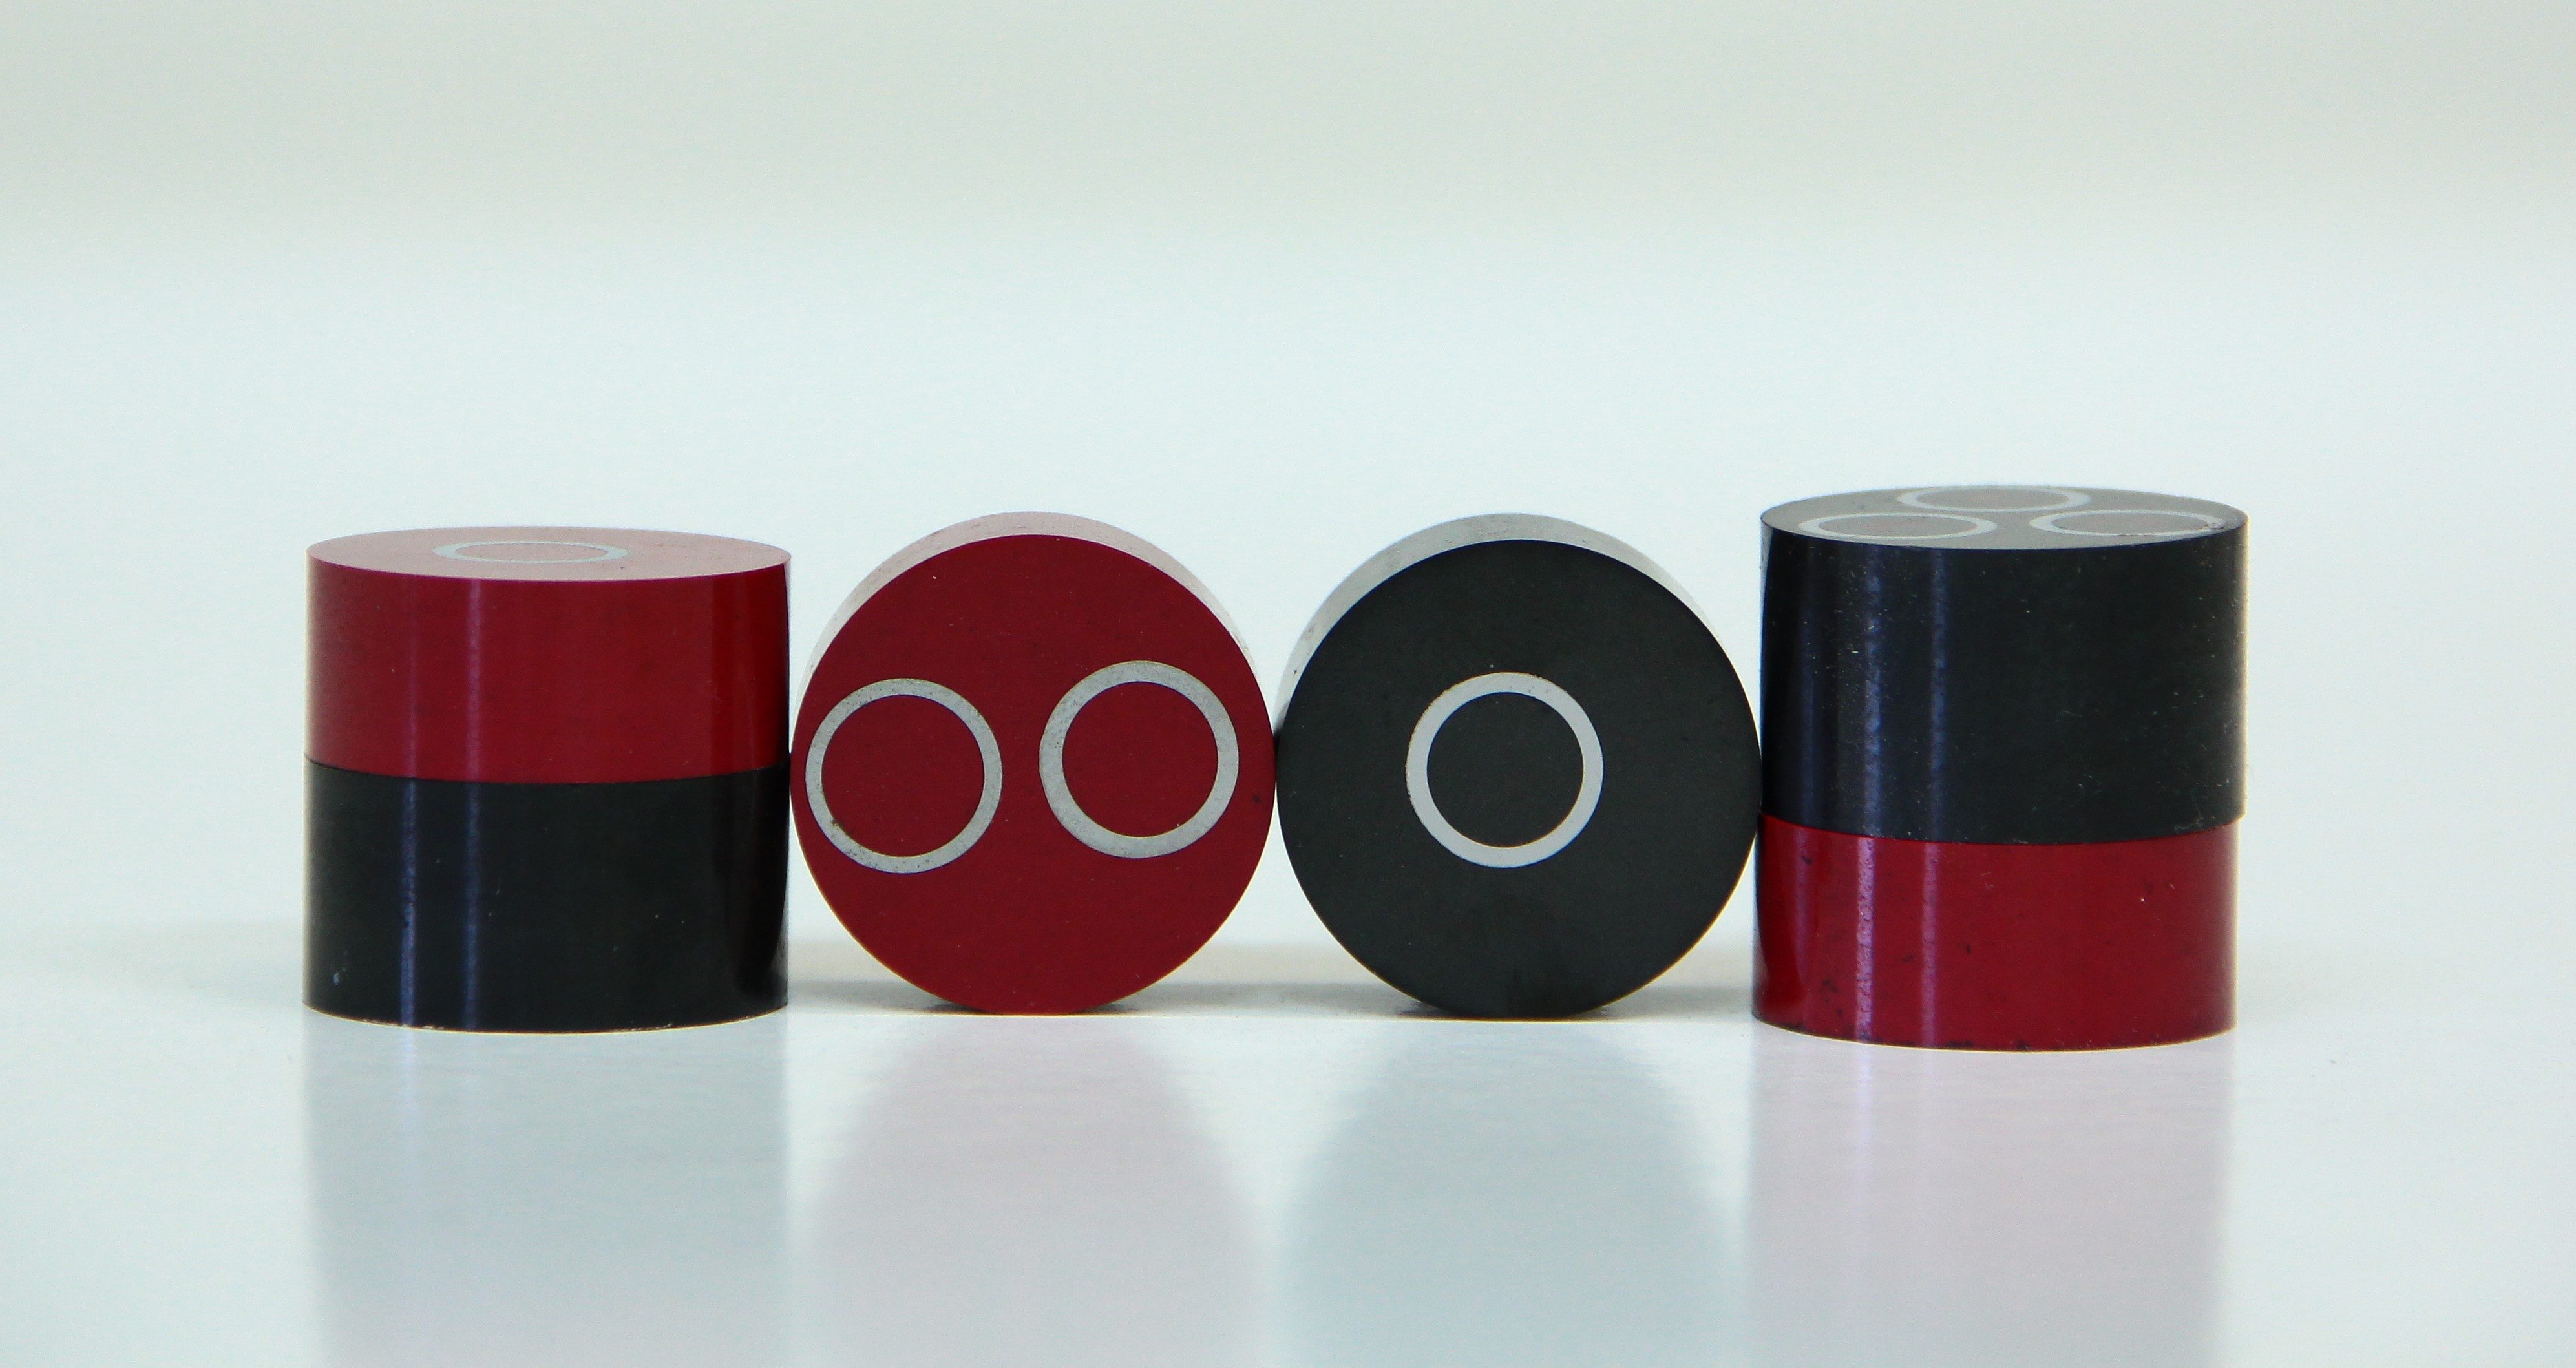
\includegraphics{images/img16.png}
\caption{Campioni inglobati in resine termoindurenti}
\labfig{img16}
\end{marginfigure}

Quest’operazione viene svolta per vari motivi:
\begin{enumerate}
    \item il campione è difficile da maneggiare: ad esempio, lamiere molto sottili, spilli, frammenti, piccole quantità di materiale;
\item il bordo del campione deve essere protetto, poiché contiene molte informazioni: nelle operazioni successivi, la superficie viene resa piana per abrasione e si rischia il distaccamento del bordo, perdendo informazioni utili sul materiale;
\item nel momento dell’analisi al microscopio si deve avere una superficie piana. Durante il processo di lucidatura, è facile applicare una pressione maggiore in un punto piuttosto che in un altro, causando la curvatura della superficie: ciò si traduce in un’impossibilità di mettere a fuoco il campione nella sua interezza;
\item potendo scrivere nel cilindro, si può identificare, etichettare e classificare il campione.
\end{enumerate}

Nel caso in cui il materiale non possa essere riscaldato a temperature al di sopra dei 120-130°C, come le leghe di alluminio serie 2000/7000/8000, poiché tale temperatura corrisponde alla loro temperatura di invecchiamento, non possono essere utilizzare resine termoindurenti. Esse vengono sostituite da \textbf{resine bicomponenti}, formate da due sostanze che messe a contatto polimerizzano a freddo, cioè a temperatura ambiente, inglobando il campione e non è necessario l’uso della pressa. Tuttavia, tali resine bicomponenti presentano una polimerizzazione inferiore a quella dei termoindurenti.

Esistono anche delle resine di \textbf{materiale elettricamente conduttivo}, che servono per preparare campioni da analizzare al microscopio elettronico. Infatti, se il materiale non fosse reso elettricamente conduttivo, si comporterebbe come un condensatore, scaricando le cariche. Oltre a tali resine, è possibile anche effettuare una \textbf{metallizzazione}\index{metallizzazione}, cioè depositare una patina di oro o grafite sulle superficie per rendere il materiale conduttivo oppure costruire un ponte di rame.\\

La superficie viene preparata e resa piana attraverso carte abrasive, mettendo in movimento reciproco la carta e il campione. Un disco di carta abrasiva ruota e spiana la superficie del campione, che è fermo. Il materiale abradente della carta abrasiva è composto da carburo di silicio e le carte hanno varie granulometrie: di solito si inizia con carte grossolane, con pochi carburi (60).\\
Esse sono classificate tramite grid, che esprimono il numero di particelle nell’unità di superficie. Come liquido lubrificante si utilizza l’acqua.\\
Per abradere la superficie si parte dalla carta più grossolana e il disco gira fino a quando vengono rimosse le tracce della lavorazione precedente. Si vedranno, alla fine del primo step, solo archi di cerchio che ricoprono la superficie: viene, quindi, lavato il campione, ruotato di 90° e viene inserita una carta abrasiva più fine. L’operazione viene effettuata fino a quando tutti gli archi di cerchio della prima carta vengono eliminati e così via. Si passa da 60, a 120, a 240, a 320, a 500, fino a 1000 e si interrompe la lavorazione quando sono presenti sulla superficie solo finissimi archi di cerchio.

Finita la lucidatura si passa ai cosiddetti panni, cioè dischi di velluto i quali hanno lo scopo di rifinire e eliminare le striature rimanenti, utilizzando come materiale abradente una pasta diamantata di varia granulometria (7 micron, 3 micron, 1 micron e 1/4 di micron) e come liquido lubrificante l’alcol dietilico. Non si usa più l’acqua perché potrebbe ossidare la superficie e perché contiene delle impurità che potrebbero rigare e graffiare il campione.

Si ottiene, così, un campione speculare, cioè uno specchio, pronto per essere analizzato al microscopio.

Un’alternativa all’uso di carte abrasive e paste diamantate è l’utilizzo dell’allumina: attraverso una sospensione acquosa di allumina si ottiene un materiale molto lucidante. Tuttavia, si tratta di una sospensione molto lattiginosa, che rischia di sporcare tutto il laboratorio.

\section{Analisi microscopica}

Finito di preparare il pezzo, si può analizzare il campione al microscopio: tipicamente quello che si vede è un cerchio bianco (cerchio perché l’oculare è di forma circolare, altrimenti si avrebbe la corrispondente forma di oculare), in quanto si ha un raggio di luce riflesso. Se la superficie contiene degli elementi non metallici, quali ossidi, solfuri di magnesio (strisce allungate), essi non riflettono la luce e si vedono come parti scure.

Nel caso delle \textbf{ghisa} si possono vedere delle macchie nere dovute alla presenza di grafite, che è una fase non metallica. Quindi, l’analisi microscopia permette uno studio della morfologia della grafite. Ad asempio, nella lega alluminio-silicio, si può studiare la distribuzione di silicio all’interno del reticolo.
Naturalmente l’analisi microscopica è molto importante anche per lo studio dei difetti, quali inclusioni e cricche.
\begin{marginfigure}[-2.5cm]
\includegraphics{images/img17.png}
\caption{Ingrandimento al microscopio ottico di un campione di ghisa}
\labfig{img17}
\end{marginfigure}

In un microscopio ottico industriale, tipicamente l’ingrandimento arriva a 1000X. Andando oltre, si ingrandisce semplicemente un’immagine, perdendo in definizione.
Per le ghise, bastano anche 100 ingrandimenti e non è necessario inglobare il campione.

A questo punto di procede con l’operazione di attacco, chimico od elettrochimico.\\
Si immerge il campione in un debole reattivo: in ambito industriale si utilizza il \textbf{NITAL}\index{NITAL}, una soluzione di acido nitrico con tenore dell’1\% in alcol etilico al 5\%, per un tempo limitato di 10-20-60 secondi. Esso deve essere poco reattivo, cioè debolmente aggressivo, perché deve reagire selettivamente: la corrosione avviene per prime le zone a maggior reattività, che sono quelle a maggior energia.

Le zone più reattive sono innanzitutto i bordi di grano: dopo l’attacco si vedranno i bordi di grano e quindi, la struttura del materiale, come nel caso degli acciai ferritici. Si possono studiare, quindi, la dimensione e la tipologia dei grani e la presenza o meno di cementite.

Nel caso di perlite, che è una miscela bi-fasica formata da ferrite e cementite, si vede una zona corrosa a causa della nascita di una pila di corrosione, cioè un anodo e un catodo dovuta alla presenza di due fasi. In questo caso si vedranno zone bianche di ferrite con bordo nero corroso e zone scure di perlite nera, a forma di lamelle corrose.

L’analisi microscopica con microscopio ottico permette di studiare la struttura morfologica e le fasi presenti in un determinato materiale metallico: permette un’analisi quantitativa e qualitativa del materiale.

\begin{marginfigure}[-8cm]
   \includegraphics{images/img18.png}
   \caption{Visualizzazione dei bordi di grano in seguito ad un attacco chimico.}
   \labfig{img18}
\end{marginfigure}
   \begin{marginfigure}[-3cm]
   \includegraphics{images/img19.png}
   \caption{Perlite al microscopio ottico}
   \labfig{img18}
   \end{marginfigure}

\section{Microscopio elettronico}\index{microscopio elettronico}

Il principio di funzionamento del microscopio elettronico è basato sull’utilizzo di un fascio di elettroni. In questo caso, il campione non necessita di una superficie riflettente e piana, ma deve essere preparato attraverso una \textbf{perfetta pulizia}, in quanto viene messo sottovuoto. Se il campione fosse sporco, le impurità inquinerebbero il tubo dove vengono emessi gli elettroni.
Il campione viene posto in una soluzione e sottoposto ad ultrasuoni che, vibrando, puliscono il campione.\\
Inoltre, esso deve essere \textbf{conduttivo}, attraverso la metallizzazione con pellicola di oro o di grafite, o l’utilizzo di un ponticello elettronico in rame.

A questo punto il materiale da analizzare viene posto in un tubo, detto \textbf{cannone}, composto da due camere, in una delle quali viene fatto il vuoto. Il filamento presente all’interno del tubo si scalda emettendo un fascio di elettroni che investono il campione: essi vengono riflessi e raccolti per mostrare la topografia del campione.

Esistono microscopi TEM\index{microscopio TEM} (\textbf{Transmission Eletronic Microscope}), utilizzati per ricerche scientifiche dove il campione deve essere così sottile da essere attraversato dagli elettroni. Se non si riesce a renderlo sottile a sufficienza, si utilizza la replica, cioè si copia la superficie su un altro materiale attraverso una pellicola. Tali microscopio raggiungono ingrandimenti da 100000X in su e sono utilizzati per ricerche fini e costose.\\
Vi sono, poi, i microscopi SEM\index{microscopio SEM} (\textbf{Scanning Eletronic Microscope}), chiamato così perché gli elettroni passano per strati mandando l’immagine a video, cioè il campione viene scansionato.

Il microscopio ottico permette di visualizzare un campo 2D, a causa della spianatura della superficie.

Il microscopio elettronico ha il grande vantaggio di dare come risultato immagini tridimensionali, dunque non c’è bisogno della superficie perfettamente piana. Avendo a disposizione la profondità di campo, tale microscopio viene utilizzato nello studio delle superfici di frattura e nello studio della fatica.\\
Infatti, nel caso di una frattura, per utilizzare il microscopio ottico, bisognerebbe spianare la superficie, perdendo le informazioni necessarie all’analisi.

I microscopi elettronici sono dotati di \textbf{microsonde}, che permettono un’analisi chimica
puntuale del materiale: se gli elettroni collidono con il materiale, esso fungerà da anticatodo e quindi da sorgente di raggi X. Ciò permette lo studio della composizione chimica del materiale attraverso un’analisi di fluorescenza: infatti, il reticolo è noto, cioè sono note le costanti reticolari, e con la legge di Bragg si può ricavare la lunghezza d’onda della radiazione emesse e di conseguenza l’energia.

Grazie a questa proprietà i microscopi elettronici sono utili per una topografia 3D della superficie e ancora di più per effettuare analisi chimiche.
\setchapterpreamble[u]{\margintoc}
\chapter{Proprietà magnetiche}
\labch{cap5}

Le proprietà magnetiche riguardano solo una particolare classe di materiali metallici, caratterizzati dalla presenza di \textbf{orbitali interni incompleti}: essi prendono il nome di \textbf{metalli di transizione}. Solo i gas nobili hanno gli orbitali completi, ma di solito quelli incompleti sono quelli esterni, che permettono i legami chimici.

Il ferro ha numero atomico 26 e la seguente struttura elettrica: 
\begin{equation*}
    \mathrm{1s^2\, 2s^2\, 2p^6\, 3s^2\, 3p^6\, 4s^2\, 3d^6}.
\end{equation*}
Si nota che l’orditale d è incompleto.
Gli elettroni di conduzione, cioè di valenza, sono quelli nell’orbitale 4s, che costituisce la banda di conduzione: essi possono lasciare il metallo e costituire la nube elettronica.
Le proprietà magnetiche risiedono nell’orbitale 3d: gli elettroni di tale orbitale sono fissi e rimangono legati all’atomo.

Per distinguere i materiali in base alle loro proprietà magnetiche, bisogna analizzare il loro comportamento quando sono sottoposti all’azione di un campo magnetico esterno. Possono verificarsi tre situazioni diverse:
\begin{enumerate}\index{ferromagnetismo}\index{paramagnetismo}\index{diamagnetismo}
    \item il materiale si oppone al campo magnetico esterno: si ha una reazione negativa da parte del materiale e una rarefazione del campo magnetico $\to$ \textbf{diamagnetismo}. Gli elettroni si muovono nell’atomo cercando di annullare le cariche per raggiungere la minima energia possibile. La presenza del campo magnetico esterno disturba il moto degli elettroni: essi cominceranno a ruotare in modo distorto, creando un campo magnetico interno che si oppone imposto dall’esterno;
    \item il materiale rafforza notevolmente il campo magnetico esterno: si ha una reazione positiva da parte del materiale e un rafforzamento del campo magnetico $\to$ \textbf{ferromagnetismo};
    \item il materiale rafforza debolmente il campo magnetico esterno $\to$ \textbf{paramagnetismo}.
\end{enumerate}

\begin{marginfigure}[3cm]
\includegraphics{images/img20.png}
\caption{Occupazione dell'orbitale 3d del ferro }
\labfig{img20}
\end{marginfigure}
Nel caso del ferro, l’orbitale d potrebbe contenere 10 elettroni, ma ne contiene solo 6. Essi sono disposti in modo da occupare tutti gli orbitali, secondo il principio di
minima energia (massima entropia) e il principio di esclusione\index{principio di esclusione} di Pauli (regola di Huns): avremo un orbitale con due elettroni e 4 con un solo elettrone.
Avendo quattro elettroni spaiati, senza il rispettivo antagonista: essi ruotando creano un momento magnetico elementare residuo. Nella
realtà, a causa dei fenomeni di schermaggio, si creano 2,6 momenti magnetici residui, invece che 4 per ogni singolo atomo.
All’interno del ferro vi è una struttura ordinata in domini magnetici o \textbf{domini di Weiss}\index{domini di Weiss}, cioè zone caratterizzate dall’iso-orientamento dei momenti magnetici residui di tutti gli atomi presenti nel singolo dominio. Tutti i domini hanno diversi orientamenti e quindi, esternamente il materiale non ha effetti magnetici, cioè non è una calamita.
Immergendo il materiale in un campo magnetico esterno, progressivamente tutti i domini tendono a orientarsi nella stessa direzione e verso del campo magnetico esterno, rafforzandolo. Si ha dunque una situazione di iso-orientamento dei momenti magnetici residui in tutto il materiale, che caratterizza il fenomeno del ferromagnetismo.
Si raggiunge la condizione di saturazione, quando tutti i domini sono ido-orientati: la curva B-H presenta, infatti, un asintoto (vedi \reffig{img21}).
\begin{figure}[hb]
    \includegraphics[width=1\textwidth]{images/img21.png}
    \caption{Evoluzione dei domini di Weiss per effetto di un campo magnetico H, rivolto verso l'alto}
    \labfig{img21}
\end{figure}

Giunti alla saturazione, rimuovendo il campo magnetico esterno, verificare due situazioni:
\begin{itemize}
    \item il materiale ritorna alle condizioni iniziali, con la disorientazione dei domini, in modo reversibile: si parla, allora, di \textbf{materiali magneticamente dolci}. Il materiali ritorna nella sua condizione di energia minima. Se il materiale non ha difficoltà a deformarsi, cioè non oppone resistenza allo scorrimento delle dislocazioni (poco carbonio, grossi cristalli di ferro, pochi bordi di grano), si tratta di un materiale dolce, in cui i domini possono facilmente ritornare alle condizioni iniziali, riarrangiandosi. In questo caso si ottiene una \textbf{elettrocalamita}: sotto l’azione del campo magnetico il materiale diventa una calamita; una volta tolto il campo magnetico, esso diventa nuovamente inerte. I materiali dolci sono costituiti da ferro pressoché puro, in quanto il carbonio rimasto nel ferro si oppone al moto dislocativo. Si utilizzano, quindi, lamierini per trasformatori costituiti da acciai al silicio: mettendo il 4-5\% di silicio, il carbonio abbandona il reticolo dell’acciaio e le dislocazioni si muovono molto più facilmente. Il silicio, infatti, è un atomo sostituzionale, che interferisce solo con le dislocazioni a spigolo, e non interstiziale come il carbonio, che interferisce con le dislocazioni a vite e a spigolo.
    \item fenomeno dell’\textbf{isteresi}: una volta annullato il campo magnetico, il materiale rimane magnetizzato e per annullare il campo magnetico residuo bisognerà quindi applicare un campo magnetico in verso opposto. I domini del materiale rimangono orientati: si è creata una calamita. Questo comportamento è tipico dei \textbf{materiali magneticamente duri}, costituiti da cristalli fini, elementi leganti e un alto tenore di carbonio, che disturbano il movimento delle dislocazioni. Le calamite sono molto fragili, in quanto le dislocazioni non hanno possibilità di muoversi.
\end{itemize}
\index{curve di isteresi}
\begin{marginfigure}[-9cm]
\includegraphics{images/img22.png}
\caption{Curve di isteresi per materiali magnetici dolci (in alto) e duri (in basso) a confronto}
\end{marginfigure}

Fino ad ora si è ragionato a temperatura ambienti, ma cosa succede variando la \textbf{temperatura}?

 Se si raggiunge la \textbf{temperatura di Curie}\index{temperatura di Curie}, il materiale da ferromagnetico diventa paramagnetico.
E’ importante quindi che il materiale sia ferromagnetico a temperature industrialmente apprezzabili. Solo tre elementi hanno questa proprietà: il ferro (768°C), il cobalto (1115°C) e il nichel a (353°C). Quando un materiale viene scaldato fino al raggiungimento della temperatura di Curie, l’entropia diventa il fattore determinante: aumentano il disordine, i domini vengono distrutti e si annulla l’iso-orientamento al loro interno, facendo diventare il materiale paramagnetico.

Un altro comportamento magnetico è quello del ferrimagnetismo, che è una disposizione nella quale i domini non sono tutti iso-orientati, ma la risultante dei momenti magnetici residui è comunque diversa da zero, in una certa direzione.

La magnetoscopia permette di verificare se il ferro è autentico o ferritico, anche solo utilizzando una calamita: essa non si attacca nel primo caso, mentre si attacca nel secondo\sidenote{I sottomarini vengono costruiti in acciaio INOX austenitico, in modo da non attrarre bombe di profondità magnetiche. Il lettore più attento si renderà conto che fare le eliche dei motori con questo materiale porterebbe a problemi di resistenza a fatica, e avrebbe proprio ragione. Vengono in genere costruiti con INOX ferritici e schermati successivamente con qualche altro metodo}.
\setchapterpreamble[u]{\margintoc}
\chapter{Produzione dell'acciaio}
\labch{cap6}

\section{Richiami di termodinamica}\index{termodinamica}

La termodinamica è la scienza che studia le trasformazioni dell’energia, che può essere intesa come la capacità di un sistema di compiere del lavoro, sebbene questa definizione non riesca ad abbracciare tutte le forme di energia.
Esistono varie forme di energia: termica, chimica (combustione), meccanica, nucleare, elettrica, magnetica, gravitazionale, e così via.

Tutte queste forme di energia possono essere racchiuse, dal punto di vista termodinamico, in un unico termine: \textbf{l’entalpia}\index{entalpia}\sidenote{Essendo l'entalpia un potenziale termodinamico risulta sempre definita a meno di una costante arbitraria, qui omessa per brevità.} $\mathrm{\bold{H=pv +  E}}$. Dove p è la pressione, v il volume massico, e E l'energia interna.\\
L’energia entalpica era l’unica forma di energia termodinamica usata fino ai primi anni del 1800 (se si omettono forme di energia più semplici, come l'energia cinetica o quella chimica data dalla combustione).

L’espressione compiuta dal punto di vista energetico di un sistema deve tenere conto, oltre l’entalpia, di un secondo termine, \textbf{l’entropia}\index{entropia}\sidenote{Anche l'entropia è una funzione di stato: vale quindi lo stesso ragionamento fatto per H. \\ Si tenga inoltre a mente che la definizione dell'entropia così formulata è valida solo per trasformazioni reversibili, ovvero in assenza di perdite.} $\mathbf{dS=dQ/T}$.\\
Essa è una misura del disordine di un sistema, che si crea quando sovrapponiamo simultaneamente più sistemi ordinati. Quindi, il disordine, in ambito termodinamico, ha un’accezione positiva, così come la presenza di difetti, quali vacanze e dislocazioni, che permettono la deformazione plastica dei materiali metallici.\\
Un sistema disordinato contiene in sé una pluralità di sistemi ordinati ed ha più possibilità di evolvere rispetto ad uno ordinato, in quanto contiene più sistemi possibili. È probabilmente utile, in questo senso, cercare di dare un'intuizione della definizione statistica dell'entropia:\sidenote{Ludwig Boltzmann, il fisico austriaco considerato il padre della meccanica statistica, fu portato al suicidio dalle angherie dei colleghi viennesi, che non ritenevano valida l'ipotesi che un gas fosse composto da singole particelle. La struttura atomica della materia non venne di fatto accettata dai fisici fino al 1905, anno in cui un impiegato dell'ufficio brevetti di Berna (Svizzera) di nome Albert usò quest'ipotesi per dare una spiegazione del moto browniano} dato l'insieme di ogni possibile configurazione di un sistema, intesa come posizione e velocità \textit{di ogni singola particella}, l'entropia può essere interpretata come una misura della probabilità che un sistema si trovi in uno stato particolare. Risulta dunque che un sistema si sviluppi verso uno stato \textit{con maggiore probabilità di esistere}.\\
\textit{Dunque, dal punto di vista energetico, visto che il principio che regola tutti i sistemi è quello di raggiungere spontaneamente il livello minimo di energia, avere un’alta entropia significa favorire il raggiungimento di esso poiché vi è la possibilità di intraprendere diverse strade}.\\
Si definisce \textbf{energia libera di Gibbs G}\index{energia libera di Gibbs}\sidenote{You guessed it, ancora un potenziale termodinamico.} di un sistema la quantità: $\mathbf{G = H - TS}$ e contraddistingue dal punto di vista termodinamico un sistema. Infatti, da un lato vi è H, che tiene conto dell’energia potenziale e cinetica gravitazionale ed è una misura dell’energia propria del sistema, dall’altro vi è S, che è una misura dei sistemi ordinati compresenti nel sistema disordinato ed è una misura della facilità di evoluzione del sistema.\\
Tale forma di energia fu “scoperta” da Gibbs e “pubblicizzata” nel mondo da Helmholtz.

Quindi, l’effetto dell’entropia è modulato dalla temperatura, la quale smorza o amplifica il suo effetto: per minimizzare l’energia libera di Gibbs, l’ideale sarebbe avere basse entalpie ed elevate entropie, quindi un sistema molto disordinato. 
Le basse entalpie si hanno in presenza di sistemi ordinati, mentre le alte entropie in presenza di sistemi disordinati.\\
Quindi il fattore determinante è la temperatura, la quale fa propendere verso l’ordine o il disordine. Infatti, avere elevate entropie se la temperatura è bassa, ad esempio a 0 K, è inutile: in questo caso, si avranno situazioni di ordine perfetto, in cui il materiale sarà caratterizzato da superconduttività, supermagnetismo poiché il reticolo è perfetto.
Ad alte temperature, invece, si avranno elevate entropie, avendo così sistemi disordinati.\\
Questo si traduce, ad esempio, nei vari stati di aggregazione che la materia può assumere: ad alte temperatura prevalgono i sistemi disordinati, come lo stato gassoso (sistema a più elevate entropia) e lo stato liquido, mentre a basse temperature prevalgono quelli ordinati, cioè lo stato solido (\reffig{img41}).
\begin{figure}[!hbt]
    \includegraphics[width = 0.6\textwidth]{img41}
    \caption{Esempio dell'andamento dell'energia libera di Gibbs in funzione della temperatura per fasi solide, liquide e gassose. Fornita da Andrea Fiori.}
    \labfig{img41}
\end{figure}

Un altro esempio è anche la modalità in cui gli elettroni vanno a riempire gli orbitali atomici o la rottura dei domini magnetici, che avviene quando la temperatura supera la temperatura di Curie: in questo caso prevale l’entropia e quindi, un sistema disordinato.

Infine, anche nel caso delle soluzioni solide si risente dell’effetto dell’entropia: considerando ad esempio gli ottoni, cioè soluzione solide di rame e zinco, si può vedere come a basse temperature si formi un ottone del primo tipo, dove lo zinco è solubile al 39\%: si tratta di una lega duttile, malleabile e lavorabile. Se si supera il limite di solubilità, si formano le fasi $\beta$ e $\beta$’. Al 50\% circa di Zn, $\beta$’ è una soluzione solida ordinata, cioè ha un reticolo CCC.\\
Se si superarono la temperatura di 454°C, la soluzione solida diventa disordinata, pur non variando la composizione chimica.

\begin{marginfigure}[-5cm]
\includegraphics{images/img23.png}
\caption{Porzione del diagramma di fase Cu - Zn a basse percentuali di Zn}
\labfig{img23}
\end{marginfigure}

\subsection{Vacanze}

Le vacanze sono difetti di reticolo puntuali e sono caratterizzate dalla mancanza di un atomo in una posizione reticolare dove, invece, dovrebbe essere presente. Le vacanze sono fondamentali perché facilitano il moto di diffusione (per vacanze) ed inoltre, hanno la proprietà di essere termodinamicamente prevedibili.\\
Le vacanze possono essere create dal passaggio di atomi dall’interno del cristallo verso la superficie. Possono muoversi dentro il cristallo in conseguenza del salto di un atomo da una posizione intorno alla vacanza, entro la vacanza stessa.

Per creare una vacanza serve un certa quantità di energia, necessaria a:
\begin{enumerate}
    \item vincere le forze esercitate dagli atomi sull'atomo che si muove;
    \item compiere il movimento stesso.
\end{enumerate}

Il lavoro, quindi l’energia, è fornito dalle vibrazioni termiche del reticolo cristallino, le quali dipendono dalla temperatura.

L’entropia è una funzione probabilistica ed una misura delle possibili configurazioni ordinate di un sistema, le quali convergono verso il minimo di energia. Le possibilità di evoluzione di un sistema sono, in genere:
\begin{itemize}
    \item miscela, un insieme di atomi con un certo numero di vacanze;
    \item reticolo perfetto con vuoti.
\end{itemize}


La presenza di vacanze incrementa l’entropia della miscela a causa di due contributi: l’entropia intrinseca e l’entropia di miscela, definita come
\begin{equation*}
    \mathrm{S_m=-(n_0-n_v)K\Big[\frac{n_v}{n_0+n_v}\ln{\Big(\frac{n_v}{n_0+n_v}\Big)}+\frac{n_0}{n_0+n_v}\ln{\Big(\frac{n_0}{n_0+n_v}\Big)}}\Big]
\end{equation*}

Dove K è la costante di ltBoltzmann ($\mathrm{K = 1,380649\cdot 10^{-23}JK^{-1}}$), $\mathrm{n_0}$ è il numero di atomi e $\mathrm{n_v}$ quello di vacanze.

Quindi, possiamo modificare l’espressione dell’energia libera di Gibbs per le vacanze:
\begin{equation*}
    \mathrm{\bold{G_m=n_vW_vT\Delta S_m}}
\end{equation*}

con $\mathrm{W_v}$ lavoro necessario per formare una vacanza e $\mathrm{\Delta S_m}$ è l’entropia della miscela che dà un’idea di quale sistema è più probabile che si verifichi.\\
Quindi, il numero delle vacanze cercherà di raggiungere per ogni temperatura un valore corrispondente a un minimo di $\mathrm{G_v}$.\\
La stessa trattazione per le vacanze può anche valere anche per quanto riguarda la quantità di lavoro necessaria per introdurre gli atomi di carbonio nel reticolo del ferro. L'espressione darà la solubilità del carbonio nel ferro, ottenendo cioè un tratto del diagramma di stato Fe-C. Il diagramma Fe-C è la sovrapposizione di quello ferro-cementite e ferro-grafite.\\
Dal punto di vista termodinamico, la presenza di cementite sarà favorita rispetto a quella di grafite, in quanto quest’ultima ha energia di attivazione molto più alta rispetto alla prima.

\section{Metodi di separazione}

In genere i metalli, siccome sono molto reattivi con l'ossigeno (sono cioè facilmente ossidabili, con alcune importanti eccezioni), vengono rinvenuti in natura sotto forma di ossidi all'interno dei minerali. È quindi necessario separare il metallo dall'ossigeno. La difficoltà di questo particolare processo è la causa dell'utilizzo di metalli particolari in epoche storiche differenti: mentre il rame può essere separato dall'ossigeno in fornaci primitive (età del rame) l'alluminio è, in questo senso, una pigna in culo.\sidenote{Il processo era talmente costoso che il servizio buono della reggia di Versailles era in alluminio.}\\
Lo studio dei metodi di separazione consiste nel valutare come varia l’energia dell’ossido al variare della temperatura.

\begin{equation*}
    \mathrm{MeO_{(solido)}\leftrightarrows Me_{(solido)}+O_{(gassoso)}}
\end{equation*}

Aumentando la temperatura, i sistemi disordinati sono più stabili, quindi l’ossido tende a dissociarsi. A basse temperature prevale la presenza dell’ossido, mentre ad alte temperature prevale la reazione di dissociazione.

Dal punto di vista cinetico, ad alte temperature è favorita la reazione di ossidazione del metallo. Dal punto di vista termodinamico, gli ossidi tendono a dissociarci in metallo e ossigeno all’aumentare della temperatura poiché aumenta l’energia libera dell’ossido, in quanto è meno stabile.\\
Diagrammando l’energia libera in funzione della temperatura, si ottengono curve monotone crescenti, che, in scala logaritmica, sono delle rette.

Nel caso dell’energia di formazione di ossidi di rame o alluminio, possiamo avere due casi:
\begin{enumerate}
    \item $\mathrm{3Cu+Al_2O_3\to2Al+3CuO}$
    \item $\mathrm{2Al+3CuO\to3Cu+Al_2O_3}$
\end{enumerate}

La reazione che avviene è la seconda, in quanto l’energia di formazione dell’ossido di alluminio è minore di quella dell’ossido di rame. Non è quindi possibile che il rame riduca l’ossido di alluminio (primo caso).\\
Osservando la figura, notiamo che la curva dell’ossido di alluminio è stabile e sta sempre al di sotto della curva dell’ossido di rame: quindi, è l’alluminio che riduce l’ossido di rame.

Tuttavia, nel ferro, l’ossigeno libero si riassopita con il metallo e si forma nuovamente l’ossido. Per conciliare il diverso comportamento termodinamico e cinetico, bisogna, quindi, introdurre un ulteriore elemento che sia in grado di reagire con l’ossigeno, che nel caso della produzione industriale deve costare poco, essere reperibile e deve avere maggiore affinità con l’ossigeno del ferro stesso.\\
Tale elemento è il \textbf{carbonio}:
\begin{itemize}
    \item $\mathrm{FeO+C\to Fe+CO_{(gassoso)}}$
    \item $\mathrm{2FeO+C\to2Fe+CO_{2(gassoso)}}$
\end{itemize}

Dal punto di vista termodinamico:
\begin{itemize}
    \item  $\mathrm{2CO\to2C+O_2}$
    \item $\mathrm{CO_2\to C+O_2}$
\end{itemize}

Nel caso del monossido di carbonio, cioè nel primo caso, il sistema più disordinato è quello dell’ossido, in quanto abbiamo due molecole di gas prima che la dissociazione avvenga: il sistema indissociato è il più stabile. Di solito, proprio il sistema dissociato è quello a entropia maggiore. Nel diagramma G-T si ha, infatti, una curva decrescente.

Nel caso, invece, dell’anidride carbonica, cioè nel secondo caso, si ottiene una molecole di gas da una molecola di gas. La retta in questo è quasi orizzontale, in quanto la reazione non dipende dalla temperatura.

Si può costruire il \textbf{diagramma di Ellingham-Richardson} (\reffig{img24}): le rette che si ottengono saranno delle spezzate a causa del cambiamento dello stato di aggregazione.
\begin{figure}[!hbt]
    \includegraphics[width=1\textwidth]{images/img24.png}
    \caption{diagramma di Ellingham-Richardson}
    \labfig{img24}
\end{figure}

Si noti che in questo grafico è molto facile ridurre l’ossido di rame: da temperature basse (80°C), il monossido di carbonio è più stabile dell’ossido di rame e quindi, semplicemente scaldando delle cupropiriti (il minerale del rame), si ha la formazione di \textbf{rame metallico}.

La temperatura a cui il ferro si riduce, invece, si aggira attorno sui 1000°C: per raggiungere queste temperature vi è bisogno un camino per il tiraggio e del mantice per rinvigorire le reazioni di combustione. In altre parole, sono necessari i forni soffiati, dove il carbonio (ottenuto in origine tramite carbone prodotto da combustione di legna) riesce così, raggiungendo temperature elevate, a ridurre il ferro. L’acciaio ottenuto artigianalmente si chiama \textit{ferro pudellato}.
\begin{figure}[!hbt]
    \includegraphics[width=0.8\textwidth]{images/img25.png}
    \caption{}
    \labfig{img25}
\end{figure}

\section{Produzione dell'acciaio}\label{steel_prod}

L’acciaio si può produrre a partire dal minerale (acciaierie a ciclo integrale) o da rottami (acciaierie elettriche).

\index{altoforno}
L’acciaio viene prodotto nell’altoforno: dal basso viene inviata aria, dall’alto invece vengono introdotti il minerale di ferro, il coke e i fondenti.\\
Il minerale deve contenere il 50\% di ferro puro.\\
Il carbone deve essere trasformato in \textbf{coke}, che è carbone quasi puro, molto robusto, in impianti chiamati cokerie. Si dispone il carbone in cataste che vengono bruciate per distillare il carbonio da tutte le impurità. La cokeria è l’impianto veramente inquinante del processo produttivo dell’acciaio.

Il \textbf{fondente}\index{fondente} è principalmente carbonato di calcio (\mathtext{CaCO_3}), che ha principalmente due scopi: il primo è quello di fluidificare la carica, cioè farla scendere con una velocità tale da far avvenire le reazioni, e per eliminare le impurità presenti nel materiale, che poi reagiscono formando le scorie dell’altoforno, chiamate loppe.

Le tre sostanze vengono pre-sinterizzate e omogeneizzate fra loro, per facilitare le reazioni, e poi caricate dall’alto.

\begin{figure}[!hbt]
    \includegraphics[width=0.8\textwidth]{images/img26.png}
    \caption{Schema della produzione dell'acciaio}
\labfig{img26}
\end{figure}

Nell’\textbf{altoforno} entra dal basso aria calda, riscaldata da quattro serbatoi detti cowpers\index{cowpers}, che sono essenzialmente degli scambiatori di calore.\\
Dato quello che esce dall’altoforno è un insieme di fumi caldi, essi vengono puliti e indirizzati nei cowpers, dove finiscono di bruciare e poi vengono espulsi come gas esausti.\\
La combustione arroventa i cowpers e quindi, viene inviata aria fredda che viene in questo modo pre-riscaldata e poi indirizzata all’altoforno, nella sacca.\\
In particolare, i quattro cowpers funzionano in modo alternato: due si preriscaldando con i gas dell’altoforno, e due invece riscaldano l’aria che deve entrare in altoforno.\\
Ciò che, infine, esce dall'altoforno sono scorie (ossidi di magnesio, di silicio, di zolfo, già presenti nel minerale. Possono essere recuperati per produrre cementi) e metallo di prima fusione, che nel caso specifico è la ghisa con un tenore di carbonio de 4,3\%\sidenote{Ovvero alla concentrazione di carbonio del punto di eutettico}.

Nella sacca arriva l’aria che reagisce con il coke formando monossido di carbonio, che salendo reagisce con il minerale.
In particolare si ha seguente successione di ossidi di ferro: 
\begin{equation*}
    \bold{\mathrm{Fe_2O_3\to Fe_3O_4 \to FeO \to Fe}}
\end{equation*}

Il ferro viene, infine, carburato formando acciaio e il prodotto che esce dall’altoforno è la ghisa.
Per produrre una tonnellata di ghisa, ne occorrono 2 di minerale, 0.9 di coke, 0.4 di fondente e 4 di aria; come prodotti, oltre alla tonnellata di ghisa, ne escono 0.8 di scorie, 5.4 di gas e 0.1 di polvere. Un altoforno può produrre circa 10000 T di ghisa al giorno.\\
Non avendo ferro puro, naturalmente nell’altoforno reagiranno tutti i materiali presenti nel materiale: si aggiungerà del sodio che reagirà con lo zolfo, per eliminare quest’ultimo, poiché non è possibile rimuoverlo all'interno del convertitore.

\begin{figure}[!hbt]
    \includegraphics[width=1\textwidth]{images/img27.png}
    \caption{Schema di un altoforno}
    \labfig{img27}
\end{figure}

\index{convertitore}
La ghisa viene trasformata in acciaio tramite un convertitore (che ha una capacità di circa 100 T), dove viene soffiato ossigeno puro e un refrattario basico, per eliminare l’eccesso di silicio e fosforo (che sono acidi). Non può essere usata l’aria perché contiene azoto. Dopodiché il materiale può essere calmato, cioè viene tolto l’ossigeno facendolo reagire con alluminio puro: si ottengono così gli \textbf{acciai calmati}\sidenote{Gli acciai non calmati sono anche detti acciai effervescenti. Sono di scarso interesse industriale perché posseggono caratteristiche meccaniche scarse}.\\
Dopo aver effettuato le opportune aggiunte, l’acciaio viene mandato in colata.\\
Si può avere la \textbf{colata in continuo}: l’acciaio mentre solidifica viene laminato in tubi di rame energicamente raffreddati, ottenendo come prodotto la cosiddetta bramma. Dopodiché si hanno le laminazioni primarie a caldo, \index{decapaggio}il decapaggio\sidenote{Bagni in acido solforico o cloridrico} per eliminare gli ossidi, e infine l’acciaio viene oliato, se è desinato alla vendite diretta, oppure viene laminato a freddo. In quest’ultimo caso, si effettuano successive operazioni di ricottura e di zincatura, per immersione o per elettrodeposizione.\\
La ricottura è necessaria perché il metallo laminato presenta dei gradi di incrudimento eccessivamente elevati. In genere una bramma deve essere tenuta in forno per circa un giorno per poter alleviare questi stress rimanenti. Il processo di ricottura lascia il materiale leggermente corrugato: viene effettuata quindi un'ultima rullatura molto blanda (detta skin milling). È possibile effettuare la ricottura in continuo, "cuocendo" la bramma srotolata in un forno lunghissimo. Questo processo ha il pregio di essere estremamente più veloce rispetto alla ricottura tradizionale, e permette inoltre di effettuare alcuni trattamenti termici già in questa fase.


\setchapterpreamble[u]{\margintoc}
\chapter{Deformazione plastica}
\labch{cap7}

Tutti i materiali si possono deformare e, generalmente, la deformazione aumenta in modo proporzionale al carico fino al punto di rottura. Questo tipo di deformazione è del tutto reversibile, essendo in campo elastico.\\
I materiali metallici hanno però in più un comportamento che si differenzia rispetto ad altri tipi di materiali\sidenote{Tipicamente i ceramici presentano solo deformazioni in campo elastico}. Infatti, superato un certo carico, anziché rompersi, cambiano comportamento e la deformazione non è più proporzionale al carico: si ha una deformazione irreversibile e si entra nel campo plastico.

\begin{marginfigure}[-5cm]
\includegraphics{images/img28.png}
\caption{Diagramma sforzo - deformazione di un materiale duttile}
\labfig{img28}
\end{marginfigure}

\index{deformazione plastica}
Questo comportamento è molto importante sia dal punto di vista produttivo che da quello applicativo: infatti, i materiali metallici possono essere lavorati sia per asportazione di truciolo, sia per deformazione plastica. Esistono tipi di lavorazioni che operano grazie a questa proprietà, come la laminazione, lo stampaggio a caldo e a freddo, la punzonatura, la calandratura, la forgiatura (il materiale viene schiacciato attraverso una pressa o una forgia, solitamente ad alte temperature).\\
La facilità di produzione è certamente molto importante, ma è il comportamento prima della frattura che rende particolarmente prezioni i materiali metallici in campo industriale. Se i materiali fragili si rompono istantaneamente, cioè senza preavviso, e in modo del tutto ingestibile, i materiali metallici prima di rompersi si deformano plasticamente\sidenote{Si definisce \textbf{duttilità} la capacità di un materiale di deformarsi plasticamente prima di giungere a rottura. Un corpo è tanto più duttile tanto maggiore è la deformazione raggiunta prima della frattura.} e quindi, danno il tempo di porre rimedio. \index{duttilità}

Inoltre, l’energia necessaria a portare a rottura un materiale, cioè l’area sottesa alla curva sforzo-deformazione fragile, nel caso di materiale fragile, ad esempio il vetro, è molto piccola, poiché la curva è molto prossima all’asse delle ordinate; un metallo invece prima di rompersi deve assorbire molta più energia\sidenote{Questa proprietà è detta \textbf{tenacità}}.\\ \index{tenacità}
\begin{marginfigure}
\includegraphics{images/img29.png}
\caption{Tenacità di un materiale fragile e uno duttile a confronto}
\labfig{img29}
\end{marginfigure}

A un certo punto, il materiale in campo plastico comincerà ad assottigliarsi (fenomeno della strizione) fino a rompersi.\\
Ciò vuol dire che i materiale metallici permettono di lavorare in perfetta sicurezza in esercizio: essi hanno carichi di snervamento $\sigma_Y$ e carichi di rottura $\sigma_R$ elevati, cioè sono materiali resistenti, che permettono un alleggerimento della struttura perché non vi è la necessità di sovrapporre molti strati. I materiali metallici hanno elevate caratteristiche meccaniche, che permettono, quindi, di ridurre il peso della struttura.\\
In caso di sollecitazione incidente, l’energia viene utilizzata per la deformazione del materiale e non per la creazione di nuove superfici, cioè non per la rottura. Affinché l’energia assorbita sia elevata, il tratto plastico deve essere molto esteso. Ad esempio, nel campo automobilistico, per la pelle delle automobili si usano materiali in fibra di carbonio, cioè materiali compositi, mentre per l’ossatura è necessario usare materiali metallici\sidenote{Emerge il problema della riciclabilità, cioè di ricaricare interamente il componente, e ciò non è possibile con i materiali polimerici e compositi. I sedili e la loro imbottitura, gli pneumatici non sono riciclabili; i materiali metallici e il vetro, invece, sono gli unici materiali totalmente riciclabili. Ora si sta diffondendo il concetto di re-impiego, cioè si utilizzano i materiali, ad esempio la carrozzeria, per fare altri accessori (declassamento meccanico).}.\\

I materiali metallici sono sicuri, ma anch’essi arrivano alla rottura. Tuttavia, ciò avviene dopo molti “campanelli di allarme”: la deformazione è visibile e per aumentarla, è necessario aumentare il carico. La velocità di deformazione è proporzionale alla velocità di aumento del carico: se il carico aumenta lentamente, la deformazione avverrà lentamente di conseguenza. Ciò permette di operare in sicurezza con i materiali metallici.

\section{Giustificazione delle caratteristiche di deformabilità: i difetti} \index{difetti}

Abbiamo detto che i vetri sono materiali fragili ed assorbono poca energia.
Se i materiali metallici fossero perfetti, non potrebbero avere le applicazioni in cui sono comunemente impiegati e sarebbero, invece, dei “super vetri”, con elevate resistenza e un carico di rottura elevato, ma comunque fragili.\\
In particolare, i difetti che permettono l’elevata deformabilità plastica sono le \textbf{dislocazioni}\index{dislocazioni}, cioè dei difetti di linea. Esse consistono nella mancanza di un semipiano nel reticolo (dislocazione a spigolo).\\
Le dislocazioni sono state prima ipotizzate e poi effettivamente scoperte. Infatti, se si calcola la tensione necessaria a deformare il materiale senza difetti ci si accorge che essa è elevatissima, al contrario di quanto dice l’esperienza.\\
Il movimento delle dislocazioni è favorito dalla presenza di sforzi tangenziali, poiché gli sforzi normali tendono a spezzare il materiale:
\begin{equation*}
    \boldsymbol{\tau = \mathrm{G}\gamma} \quad\text{sforzo tangenziale}
\end{equation*}
dove si sono considerati angoli di deformazione $\gamma$ molto piccoli, tali cioè che $\tan\gamma\simeq\gamma$.\\
Si potrebbe pensare che per determinare una deformazione permanente sia necessario spostare la fila superiore di atomi di una distanza interatomica a. Tuttavia il legame viene spezzato e ricreato con l'atomo successivo già a metà dello spostamento, determinando un angolo $\gamma\simeq1/2$. La $\tau$ teorica in questo caso vale intorno a $10^4\text{MPa}$. I dati sperimentali collocano tuttavia lo sforzo necessario a determinare una deformazione permanete intorno ai 10Mpa.\\
Il ragionamento teorico è difatti valido solo per un materiale perfetto senza difetti: si suppone il sollevamento simultaneo di tutto il piano, la rottura contemporanea di tutti i legami e la ricollocazione del piano stesso in una nuova posizione. In questo caso, si ottengono valori di tensioni molto elevate.

In realtà, con molto meno sforzo, si può creare un’ “onda” che viene fatta scorrere lungo tutto il piano: alla fine del processo, il piano si sarà spostato di una lunghezza pari alla lunghezza d’onda (esempio del tappeto). Tale fenomeno viene identificato nelle dislocazioni.

Nei legami ionici, come ad esempio il gesso (solfato di calcio biidrato $\mathrm{CaSO_4-2H_2O}$) o il sale, che ha una struttura cubica semplice, non c’è movimento dislocativo perché esso porterebbe ioni dello stesso segno a contatto, innescando immediatamente forze repulsive, che causano la rottura del materiale (il materiale si spacca).
Nel legame metallico, invece, i moti dislocativi sono permessi grazie alla presenza della nuvola elettronica: infatti, spostare uno ione non produce alcuna conseguenza.

Si definisce \textbf{vettore di Burgers}\index{vettore di Burger}, \textbf{b}, il vettore che indica lo spostamento delle dislocazioni. Le dislocazioni si muovo lungo direzioni che rendono il vettore di Burgers il più piccolo possibile, poiché l’energia necessaria da fornire affinché una dislocazione si muova è proporzionale a \mathtext{b^2}. Tali piani sono quelli in cui gli atomi sono più vicini, ovvero le distanze interatomiche sono minori: si tratta dei piani a maggiore densità elettronica.\sidenote{Nei reticoli CFC e EC, il vettore di Burgers b è diverso dalla distanza reticolare a e si parla di dislocazioni parziali.}

Nel caso di una cella cubica a facce centrate CFC, i piani con gli atomi più vicini sono quelli diagonali (1 1 1), cioè il piano passante per i tre vertici, nelle tre direzioni <1 $\overline{1}$ 0>. Per ogni cella sono quindi consentiti movimenti in tre direzioni su quattro piani differenti, determinando 12 possibili sistemi di scorrimento.\\
Quindi, il reticolo CFC è quello più sicuro poiché la deformazione avviene in ogni caso. Ne è un esempio l’austenite, che è molto costosa.

Anche nel caso di una cella cubica a corpo centrato CCC, le possibili direzioni per il moto delle dislocazioni sono 12. I sistemi di scorrimento in questo caso però si possono attivare o meno in base alla temperatura. Per temperature maggiori della temperatura ambiente, tutti i sistemi sono attivi e si ha un materia duttile, mentre al di sotto della temperatura ambiente il materiale diventa fragile. Perché la temperatura influenza il moto dislocativo e di conseguenza, la deformazione plastica? All’aumentare delle temperatura aumentano le vacanze che favoriscono il movimento dislocativo.\\
Se vi è un ostacolo, la dislocazione cambia piano di scorrimento: la dislocazione a vite è parallela al vettore di Burgers; quindi può facilmente cambiare piano; la dislocazione a spigolo, invece, è perpendicolare al vettore di Burgers e il piano di scorrimento (all’interno del quale è sempre contenuto il vettore \textbf{b}) è proprio il piano individuato da essi: la dislocazione, quindi, non può cambiare piano.\\
 \textit{Vedi lucidi fenomeni di rafforzamento}.

Esistono dei meccanismi di rafforzamento\index{meccanismi di rafforzamento} per inibire il moto dislocativo:
\begin{enumerate}
    \item  includere nel reticolo di atomi sostituzionali e/o interstiziali: gli atomi interstiziali hanno maggiore potere penetrante e quindi interagiscono sia con le dislocazioni a spigolo sia con quelle a vite, mentre i sostituzionali solo con quelle a spigolo;
    \item incrudimento\index{incrudimento}: le dislocazioni creano altre dislocazioni che interagiscono fra loro, creando degli ingorghi;
    \item  raffinamento dei grani, più il grano è piccolo, più salti vi sono da fare e quindi, deve aumentare il carico. I bordi di grano sono infatti in grado di ostacolare il moto delle dislocazioni. Tale meccanismo aumenta anche la tenacità, bloccando la propagazione delle cricche. Se il grano è grosso, si ha una frattura a nucleazione limitata, dato che una sola cricca può attraversare tutto il grano e rompere il materiale. Se i grani sono piccoli, per portare a rottura il materiale servono più cricche, portando una frattura a propagazione limitata. La rottura dovuta al moto dislocativo avviene a 45°.
\end{enumerate}

\section{Tratto elasto-plastico}

Definiamo il carico nominale: $\sigma_n=\mathrm{P/A_0}$, dove $\mathrm{A_0}$ rappresenta la sezione iniziale.
Definiamo l’allungamento: $\varepsilon=\Delta L/\mathrm{L_0}$\\
Quando si supera la tensione di snervamento $\sigma_Y\simeq\sigma_{02}$ inizia l’incrudimento.
Il tratto seguente viene impropriamente chiamato tratto plastico, quando dovrebbe essere indicato esattamente come tratto elasto-plastico. Quando si scarica il materiale, cioè eliminando il carico $\sigma_{02}$, esso presenta una deformazione plastica residua dello 0,2\%.\\
La retta passante per l’origine e quella passante per la tensione di snervamento in realtà non sono parallele, in quanto il modulo di Young diminuisce all’aumentare della deformazione, poiché si introducono nuove deformazione che diminuiscono la rigidezza del materiale (è come si si introducessero dei buchi nel materiale).

Si ha un effetto di \textbf{springback} o \textbf{ritorno elastico}\index{ritorno elastico}: tutta le deformazione accumulata nel tratto puramente elastico viene recuperata, determinando una deformazione minore rispetto a quella ottenuta con il carico applicato. Questo comportamento è non voluto, perché l’energia elastica viene fornita, quindi rappresenta un costo, e viene restituita in modo talvolta dannoso. Tale effetto deve essere minimizzato, ad esempio, per la produzione degli stampi, dove le tolleranze dimensionali sono minime.

Bisogna, quindi, avere carichi di snervamento bassi, in quanto così si arriva nel tratto plastico con meno sforzo, che si traduce in potenze minori nelle presse e minor ritorno elastico a parità di deformazione.

Negli \textbf{acciai da profondo stampaggio}\index{acciai da profondo stampaggio}, utilizzati per la realizzazione delle carrozzerie, il carico di snervamento è basso.\\
Inoltre, in essi vi sono pochi elementi leganti (tenore di carbonio varia tra lo 0,02\% allo 0,04\%; bassissimi tenori di nichel Ni, silicio Si e magnesio Mg) ed il grano non deve essere fine, ma grosso (comunque non oltre il 20 micron), perché quello fine blocca le dislocazioni.

Il grano deve essere grosso anche per \textbf{leghe per alta temperatura}\index{leghe per alta temperatura}, cioè per le \textbf{superleghe}. Dovendo queste operare a temperature molto elevate possono incorrere nel fenomeno del \textbf{creep}\index{creep}, dove le deformazioni plastiche sono causate non solo dal moto dislocativo, ma anche dallo scorrimento tra grani: quindi avere grani grossi minimizza questo effetto; addirittura si hanno dei precipitati a bordo grano per evitarne lo scorrimento relativo.

Questo comportamento continua fino a quando non si arriva al carico massimo, dove si verifica la una strizione: mentre prima la deformazione era uniforme, con la comparsa delle strizione essa va a localizzarsi solo in una sezione ristretta.\\
Superato il carico massimo, per avere delle deformazioni è necessaria una sollecitazione minore poiché essa agisce su un’area più piccola.\\
In un materiale perfettamente elastico, la componente plastica non va ad aumentare, e sappiamo che si comporta come un materiale fragile, cioè per sforzi maggiori al carico di snervamento, il materiale si rompe.
Quindi la componente plastica è quella che ci permette di sfruttare a pieno le potenzialità del materiale, ed anche il successivo incrudimento.

Nei diagrammi sforzo-deformazione utilizziamo sempre una tensione nominale, calcolata sulla sezione indeformata e si ha un valore nominale della deformazione, proporzionale alla lunghezza di riferimento $\mathrm{L_0}$: $\varepsilon=\Delta L/\mathrm{L_0}=\mathrm{(L-L_0)/L_0}$. Tali valori non rispecchiano l’andamento reale perché l’area varia durante la prova.

Si potrebbe, quindi, usare una tensione reale, riferita alla sezione misurata istante per istante. Dato che in campo plastico vale la legge della conservazione del volume (AL = $\mathrm{A_0L_0}$), si ha che:
\begin{equation*}
    \boldsymbol{\sigma_r}=\mathrm{\frac{P}{A}=\frac{P}{A}\frac{A_0}{A_0}=\sigma_n\frac{A_0}{A}=\boldsymbol{\sigma_n(\varepsilon+1)}}
\end{equation*}
Dove si è usata la conservazione del volume e il fatto che $\mathrm{\varepsilon+1=L/L_0}$.

Un discorso analogo può essere svolto per le deformazioni: nelle prove si misura una lunghezza iniziale \mathtext{L_0}. Quando il materiale comincia a deformarsi si ha una deformazione pari a \mathtext{(L_1-L_0)/L_0}. Nella deformazione successiva si partirà da una lunghezza iniziale $\mathrm{L_1}$ e si avrà \mathtext{(L_2-L_1)/L_1}.
La deformazione reale si può quindi scrivere come:
\begin{equation*}
    \varepsilon_r=\sum_n\frac{L_{n+1}-L_n}{L_n}
\end{equation*}

Passando all’integrale tra \mathtext{L_0} ed L si ottiene 
\begin{equation*}
    \varepsilon_r= \ln(L/L_0)=\ln(\varepsilon+1)
\end{equation*}

Visto che il logaritmo in campo elastico si può confondere con il suo argomento, vale la legge di Hooke \mathtext{\sigma = E\varepsilon}.\\
In campo plastico però la legge non è più lineare, ma vale una relazione del tipo \mathtext{\sigma_r=K\varepsilon_r^n}, dove n è il coefficiente di incrudimento, che determina la pendenza del tratto plastico.\\
\begin{marginfigure}[-4cm]
\includegraphics{images/img30.png}
\caption{Diagramma sfrozo - deformazione reali}
\labfig{img30}
\end{marginfigure}
Nel caso reale, vi è una diminuzione del carico perché si continua a considerare la sezione iniziale \mathtext{A_0}, mentre nella realtà non vi è un massima apparente, ma si hanno curve monotone crescenti, in cui non è evidente il carico massimo.\\
Se n=0 avremo un materiale perfettamente plastico (caratterizzato da una curva $\sigma-\varepsilon$ orizzontale), se invece n=1 avremo un materiale perfettamente elastico. Dunque nella realtà 0<n<1.\\
Si cerca di avere un materiale con il coefficiente di incrudimento più alto possibile, perché all’aumentare di n aumenta anche la differenza di carico permessa nel tratto plastico, il che si traduce in una maggiore facilità di lavorazione.

In condizione di carico massimo, si ha:
\begin{align*}
    & (dF)_{max} = 0 \Rightarrow \sigma dA + A d\sigma = 0 \Rightarrow \frac{d\sigma}{\sigma} = -\frac{dA}{A}\\
    & \text{Vol. cost} \Rightarrow ldA + Adl = 0 \Rightarrow \frac{dA}{A} = -\frac{dl}{l}\\
    & \frac{d\sigma}{\sigma} = \frac{dl}{l} = d\varepsilon \Rightarrow \boxed{\frac{d\sigma}{d\varepsilon} = \sigma}
\end{align*}
 la derivata della tensione rispetto alla deformazione è uguale alla tensione stessa e in particolare, introducendo l’espressione di \mathtext{\sigma_r} in condizioni di carico massimo, si ottiene che \mathtext{\varepsilon_{F_{max}}=n}.\\
Infatti, a parità di carico di snervamento, se aumenta n, aumenta anche la deformazione a carico massimo, quindi il materiale è molto più deformabile e stampabile.

Ricapitolando, per avere un \textbf{materiale facilmente stampabile}, bisogna avere basse tensioni di snervamento, alti coefficienti di incrudimento, elevati moduli elastici (per evitare il ritorno elastico) ed elevato coefficiente di anisotropia R\index{coefficiente di anisotropia}.

L’anisotropia è una misura di quanto le proprietà sono le stesse in ogni punto del materiale.
Si definisce coefficiente di anisotropia R la quantità:
\begin{equation*}
    \mathtext{R = (D_{longitudinale} + D_{trasversale} + 2D_{45°}) / 4 = (L + T +2D_{45°}) / 4}
\end{equation*}
D indica la deformazione, L è la deformazione longitudinale e T è la deformazione trasversale.

Un materiale deformato solitamente si allunga nella direzione di applicazione del carico e si assottiglia nelle altre due direzioni. Nel caso di lamiere sottili (1 mm, 0.8 mmm, 0.6 mm) è pericoloso se esse si assottigliano troppo nel senso dello spessore, poiché diminuisce la resistenza della struttura (fenomeno dello \textbf{stone chipping}, ovvero la perforazione di marmitte o pezzi meccanici posti sotto la carrozzeria a causa dei sassi lanciati dagli pneumatici).

E’ preferibile avere R molto elevato, cioè un manufatto che si allunga, ma non si assottiglia.\\
Per sfavorire l’assottigliamento bisogna inibire la crescita dei piani dove si muovono le dislocazioni nel senso dello spessore.

Nella produzione degli acciai, in fase di produzione si ha prima un’ossidazione nel convertitore e poi il calmaggio. Si introduce dell’alluminio Al, che in parte forma dell’ossido portando via dell’ossigeno, ma una percentuale dello 0,04\% rimane nell’acciaio. Tale tenore di alluminio è responsabile dell’anisotropia: infatti, si formano nitruri di alluminio (Al + N), che rimangono in soluzione nell’acciaio, cioè rimangono intrappolati.\\
Dopo il calmaggio, si ha una laminazione a caldo alla temperatura più alta possibile per evitare la precipitazione di tali nitruri. Per arrotolare successivamente la lamiera, bisogna mantenersi a temperature basse, sempre per evitare la precipitazione di tali nitruri.\\
Si può così effettuare la laminazione a freddo, a seguito della quale si ha una ricottura, ad una temperatura di circa 700 - 750 °C, durante la quale deve precipitare il nitruro di alluminio.
\setchapterpreamble[u]{\margintoc}
\chapter{Diagramma di stato Fe-C}\label{Fe-C}
\labch{cap8}

Il ferro puro presenta due diverse forme allotropiche:
\begin{itemize}
    \item configurazione CCC a 907°C;
    \item CFC da 907°C a 1394°C;
    \item CCC fino alla temperatura di fusione di 1537°C.
\end{itemize}

In presenza di \textbf{carbonio}, che è un elemento austenitizzante, cioè un elemento che stabilizza la fase austenitica e ne ampia l’esistenza, le forme allotropiche cambiano e si originano diverse \textbf{soluzioni solide}. Si ha:
\begin{itemize}
    \item \textbf{ferrite} \mathtext{\boldsymbol\alpha}, in cui la solubilità di carbonio è 0,02-0,03\% a 723°C nella configurazione CCC;
    \item \textbf{austenite} \mathtext{\boldsymbol\gamma},  in cui il tenore di carbonio è del 1,98-2\% a 1130 °C (1135 °C) nella configurazione CFC;
    \item \textbf{ferrite} \mathtext{\boldsymbol\delta}, n cui la solubilità massima del carbonio è dello 0,1\% a 1492°C configurazione CCC. La maggior solubilità del carbonio nell’ultima configurazione rispetto alla ferrite \mathtext{\alpha} deriva dalle dilatazioni termiche.
\end{itemize}

L'aggiunta di elementi leganti può portare ad un aumento o ad una diminuzione del campo austenitico. Sono elementi austenitizzanti (ovvero che aumentano il campo di esistenza del ferro $\gamma$) il carbonio, il nichel, il manganese, l'azoto. Il cromo è invece un elemento ferritizzante (aumenta il campo di esistenza del ferro $\alpha$ e $\delta$.)

\begin{figure}[h]
\centering
    \includegraphics[width=1\textwidth]{images/img31.png}
    \caption{Diagramma Fe-C per percentuali di C inferiori al 6,69\% (cementite)}
    \labfig{img31}
\end{figure}
\index{peritettico}
\textbf{PERITETTICO (punto I): Liquido (0,18 \%C) + ferro \mathtext{\boldsymbol\delta} (0,1 \%C)→ austenite \mathtext{\boldsymbol\gamma} (0,5 \%C)}\\
La trasformazione peritettica avviene a 1492 °C con tenore di carbonio pari allo 0,18\%. Nel peritettico vi è la trasformazione di una fase solida, cioè l’austenite, sottoposta a riscaldamento, in una fase liquida e una solida, cioè la ferrite \mathtext{\delta}.\\
Il punto peritettico è importante nei fenomeni di solidificazione.\\
Esso infatti da origine a due fenomeni.\\
Si può avere il \textbf{salto del peritettico}, se la trasformazione non avviene in condizioni di equilibrio, cioè non avendo la presenza di un liquido con 0,5\% di carbonio e un solido con tenore 0,1\% di C. Si ha una zona stratificata con bande di liquido e solido, con la parte liquida più all’interno in quanto solidifica più lentamente. Tale fenomeno prende il nome di \textbf{bandizzazione} o \textbf{stratificazione}.
L’altro fenomeno è la \textbf{differente cristallografia e morfologia} tra superficie e cuore del lingotto. In superficie si originano dei cristalli molto piccoli e fini perché siamo in presenza di elevata nucleazione di cristalli; nelle zone sotto la superficie i cristalli si allungano dando vita a una struttura dendritica a palizzata; infine nel cuore vi è una struttura poligonale. Ci si può trovare davanti, quindi, ad un materiale che è chimicamente e cristallograficamente disomogeneo.\\
A questo problema si può ovviare tramite la \textbf{ricottura}, in modo da omogeneizzare completamente la struttura, e tale processo prevede un riscaldamento del lingotto fino alla temperatura più alta possibile (a circa 1200°C) e successivo raffreddamento lento. In realtà la ricottura avviene solo per acciai di altissimo pregio: infatti, le colate non avvengono più in lingotteria, da cui si originano i lingotti, ma si preferisce utilizzare la \textbf{colata in continua}, in cui la solidificazione avviene simultaneamente alla prima laminazione. Non appena si forma una pellicola di solido sufficientemente spessa e tale da resistere ad azioni meccaniche, si comincia a laminare. Il prodotto in uscita dalla colata in continua si chiama \textbf{bramma}, cioè il grezzo di colata che ha già subito la prima laminazione. Non si ha in tal modo la struttura a palizzata e si sfrutta il calore del materiale che sta solidificando e che cede calore all’aria.

\index{eutettico}
\textbf{EUTETTICO (punto C): Liquido (4,30 \%C) → austenite + cementite \mathtext{Fe_3C} o grafite}\\
La trasformazione eutettica avviene a \textbf{1130°C} con tenore di carbonio pari al 4,3\%: si ha del liquido che, solidificando (raffreddamento), si trasforma in austenite più una fase che a seconda delle condizioni può essere o grafite o cementite.\\
Se il raffreddamento è lento e non vi sono elementi grafitizzanti, allora la trasformazione eutettica porta alla formazione di austenite e cementite. Se, invece, il raffreddamento è comunque lento, ma sono presenti elementi grafitizzante, allora si forma la grafite.\\
Qualora la seconda fase sia la cementite, la miscela formata da austenite e cementite è chiamata \textbf{ledeburite}.

\index{acciaio}
Se si supera il punto E, con \%C pari a 2,2\%, si entra nel campo delle \textbf{ghise}. Se la \%C è inferiore al 2\%, cioè siamo nel campo degli \textbf{acciai}, essi non sono interessati alla trasformazione eutettica, cioè nella solidificazione non è presente l’eutettico. Tuttavia esistono acciai speciali con \%C > 2, cioè gli acciai refrattari, e anche ghisa con \%C < 2.

Le ghise sono dei materiali la cui caratteristica principale è la colabilità, sono cioè \textbf{leghe da getto}. Con le ghisa, si cerca di ottenere il manufatto il più possibile simile al risultato finale a ridosso della solidificazione, per ridurre il più possibile le lavorazioni successive.\\
Il requisito per una \textbf{facile colabilità} è quello di avere una temperatura di colata e di solidificazione più basse possibili, temperature che corrispondono a quella del punto eutettico, che è il punto nel quale vi è liquido alla temperatura più bassa possibile. In questo punto si passa da un 100\% di liquido a 100\% di solido, mentre in tutti gli altri punti si ha la coesistenza di liquido e solido: quindi nel punto eutettico non si ha un intervallo di solidificazione. Attraverso la colata, si posso realizzare pezzi dalla forma complessa.\\
Se si ha la coesistenza di liquido e solido ci si trova in presenza di un \textbf{fango}, che ha elevata viscosità, con il rischio che esso non riempia bene lo stampo, ottenendo di conseguenza dei getti difettosi. Quindi tutte le volte che si ha un materiale da getto (ghisa, ottone, bronzo, leghe d’allumunio) la \textbf{composizione} deve essere quella \textbf{più vicina possibile a quella dell’eutettico}. Infatti, maggiore è l’intervallo di solidificazione, maggiori sono le probabilità di avere fanghi e di conseguenza, stampi difettosi.

In realtà, se si colasse una ghisa con tenore di carbonio 4,3\% (cioè quella che esce dall’altoforno), essa sarebbe troppo fragile, con modestissime caratteristiche meccaniche.
Utilizzando, però, un tenore di carbonio inferiore, quindi muovendosi verso sinistra nel diagramma di stato, si avrebbe la solidificazione dell’austenite, con formazione di cristalli austenitici, e il carbonio si andrebbe a posizionare a bordo di grano, infragilendo ulteriormente il materiale.
La soluzione di questo problema si ha aggiungendo un terzo elemento, cioè il \textbf{silicio}\index{silicio}. Si ottengono, così, le ghise al ferro-carbonio-silicio.\\
Questo elemento aumenta l’attività del carbonio, cioè, in presenza di silicio, il carbonio diventa più attivo e si comporta come se ce ne fosse di più della sua reale quantità. Il silicio è un \textbf{attivizzante di carbonio C}. L’effetto energizzante è di 1:3, cioè 3 parti di silicio fanno si che il carbonio si comporti come se ce ne fosse una parte in più (0,3\% Si \mathtext{\to} + 0,1\% di C). Mettendo il 3\% del silicio, e calcolando il carbonio equivalente si arriva a un tenore di carbonio che è 4,3\%, quando nella realtà il carbonio effettivamente presente è circa del 3\%. Tale tenore di carbonio è accettabile dal punto di vista meccanico.

Un’altra tecnica utilizzata in questo ambito, oltre alla modifica della composizione chimica, è la cosiddetta \textbf{inoculazione}, che serve ad avere grafite che, sotto forma di lamelle, è uniformemente distribuita nella ghisa, che è chiamata in questo caso \textbf{ghisa lamellare}. L’inoculazione consiste nell’aggiungere al momento della colata un ulteriore 0,1\% di silicio sotto forma di polvere, in modo uniforme sul bagno liquido di ghisa che sta solidificando: localmente il silicio aumenta di molto l’attività di carbonio, arrivando in condizioni ipereutettiche, perché vi è l’attività energizzante del silicio. In queste condizioni, la prima fase a solidificare è la grafite, che non andrà a posizionarsi a bordo grano, ma è distribuita uniformemente su una matrice che segue il diagramma di stato Fe-C. La ghisa ha la forma di dischetto, ma in sezione ha la forma di lamella.\\
Gestendo bene l’operazione, si riesce a ottenere una distribuzione uniforme della grafite su una \textbf{matrice perlitica} (raffreddando una lega al 2\% ci carbonio) oppure, raffreddando molto lentamente, su una \textbf{matrice ferritica}.\\
La lamella di ghisa ha gli apici aguzzi con fattore di intaglio pari a 13. Ciò significa che agli apici della lamella, gli sforzi sono intensificati di un fattore pari a 13.

Una variante a questo tipo di ghisa è la \textbf{ghisa sferoidale}, dove la grafite al posto di essere in forma lamellare è in forma sferoidale. Essa presenta il vantaggio di avere un fattore di intaglio pari a 3, cioè permette di avere un materiale a basso costo con caratteristiche meccaniche più elevate e paragonabili agli acciai. Infatti, gli acciai da bonifica sono molto costosi.
La forma sferica si ottiene aggiungendo dopo l’inoculazione un ulteriore 0,1\% di \textbf{magnesio Ma}\index{magnesio}, che ha lo scopo di alterare la tensione superficiale della grafite in fase di solidificazione. La grafite così solidifica a forma sfeiroidale.\\
In questo caso è previsto un allungamento, a differenza della ghisa lamellare.

Combinando l’\textbf{aggiunta di silicio} ad un \textbf{raffreddamento lento}, si ha un’elevata \textbf{grafitizzazione}.

Se, invece, si \textbf{raffredda velocemente} con la presenza di una \textbf{bassa percentuale di silicio}, durante la trasformazione eutettica, si inibisce la formazione di grafite a favore della cementite, ottenendo le cosiddette \textbf{ghise bianche}, formate da placche di cementite.\\
Essendo la cementite una fase dura e caratterizzata da grandi cristalli bianchi, si aggiungono elementi leganti del carbonio che favoriscono la formazione dei propri carburi (vanadio, niobio) e si ottiene un materiale molto duro e poco costoso.

Tuttavia, si tende ad espellere carbonio e formare grafite.

Una via di mezzo è la \textbf{ghisa trotata}, dove si ha coesistenza di grafite e cementite, cioè il carbonio è solidificato in entrambe le forme. Tale ghisa però è uno scarto in quanto non è utile.

Nelle ghise si può avere il cosiddetto \textbf{occhio di bue}: ad esempio, nella ghisa sferoidale si ha un cerchio nero di grafite sferoidale, che contiene la maggior parte di carbonio, circondato dalla ferrite che è bianca e priva di carbonio.

\index{eutettoidico}
\textbf{PUNTO EUTETTOIDICO (punto S): Austenite \mathtext{\boldsymbol\gamma \to} ferrite \mathtext{\boldsymbol\alpha} (0,02 \%C) + cementite \mathtext{\boldsymbol{Fe_3C}} (6,66 \%C)}\\
La trasformazione eutettoidica si trova a una temperatura di \textbf{723°C} con tenore di carbonio pari allo 0,8\%. In questo punto si ha una fase solida di alta temperatura, cioè l’austenite, che al raffreddamento genera due fasi solide di differente composizione (ferrite allo 0,02\% di C e cementite al 6,66\% di C).\\
Se ci si trova proprio del \mathtext{punto eutettoidico}, la miscela meccanica che solidifica con 89\% di ferrite e 11\% di cementite è chiamata \textbf{perlite}.\\ \index{perlite}
Se \textbf{\%C < 0,8}, la ferrite \mathtext{\alpha} solidifica prima, cioè si trasforma precedentemente a causa del raffreddamento dell’austenite: quindi, si ha \textbf{ferrite e perlite}.\\
Se \textbf{\%C > 0,8}, si ha \textbf{cementite e perlite}. La trasformazione eutettoidica è:
\begin{equation*}
    \gamma(0,8\%\mathtext{C})\to\alpha(\simeq0\%\mathtext{C})+\mathtext{Fe_3C(6,66\%)}
\end{equation*}
La ferrite \mathtext{\alpha} non contiene carbonio, che invece è interamente contenuto nella cementite.

Tale trasformazione è governata dai \textbf{meccanismi di diffusione}, che a sua volta dipende dalla temperatura e dal tempo (legge di Fick), oltre che dalla forza spingente (che in questo caso è la differenza di concentrazione); l’effetto predominante è quello della temperatura perché di tipo esponenziale (\mathtext{e^{1/T}}), mentre l’effetto del tempo è sotto radice quadrata (\mathtext{t^{1/2}}).\\
Questa trasformazione avviene attraverso processi di \textbf{nucleazione}, che consiste nella formazione nuclei di ferrite e cementite, quindi creando una  \textbf{struttura lamellare}, perché la ferrite è priva di carbonio, che invece è totalmente contenuto nella cementite. Il processo successivo è la \textbf{crescita dei nuclei} con il tempo.
\setchapterpreamble[u]{\margintoc}
\chapter{Trattamenti termici}
\labch{cap9}

Si è visto nel capito precedente che i passaggi di fase dipendono sia dalla temperatura che dal tempo della sua variazione. È quindi evidente che variando il tempo di raffreddamento o di riscaldamento si otterranno risultati molto diversi. I processi termici sono caratterizzati da un riscaldamento e da un successivo raffreddamento, lento o veloce.

\section{Riscaldamento}

Riscaldando si deve arrivare a \textbf{completa austenitizzazione} se la composizione è esattamente eutettoidica (0,8 \%C a 723°C).
Per non deturpare il pezzo durante il riscaldamento ed evitare l’ossidazione\sidenote{Questo problema non si pone se il pezzo in questione è grezzo, ossia deve ancora subire delle lavorazioni. In questo caso lo strato ossidato verrà semplicemente rimosso in seguito.} (a causa della presenza dell’ossigeno che è un inquinante) e la decarbrazione, si utilizzano delle \textbf{atmosfere inerti}\index{atmosfere inerti}.
\begin{enumerate}
    \item \textbf{Gas nobili} quali Argon Ar e elio He, che però hanno un costo non indifferente. Essi si ottengono per distillazione frazionata dell’aria;
    \item \textbf{Azoto N}  che può fungere da gas nobile poiché, in linea di massima, nei trattamenti termici può essere considerato inerte. Solo negli acciai con elevato tenore di cromo Cr non si può utalre tale atmosfera, perché l’azoto reagisce con gli elementi, formando nitruri. L’azoto viene ricavato dall’aria attraverso o la distillazione dell’aria liquida oppure tramite combustione dell’aria (formazione di azoto e di anidride carbonica, l’azoto non reagisce con l’ossigeno). Tali metodi metodi hanno dei costi abbastanza elevati, che variano in base alla purezza dell’azoto.
\end{enumerate}

Tuttavia, si possono avere anche \textbf{atmosfere a basso costo}: noi sappiamo che tale reazione di combustione \mathtext{C_xH_y + O_2 \to CO_2 + H_2O} avviene in eccesso di ossigeno: la \mathtext{CO_2} non è velenosa, a differenza del monossido di carbonio (a meno che non saturi l’atmosfera).\\
Se facciamo avvenire tale reazione in \textbf{rarefazione di ossigeno}, si ha la seguente reazione di combustione:
\mathtext{C_xH_y +O_2 \to CO_2 +H_2O+H_2 +CO}
con i termini a destra che in generale prevengono l'ossidazione. Sono detti \textbf{gas endotermici}\index{gas endotermici}. Si ha infatti la reazione:
\mathtext{CO + H_2O \to CO_2 + H_2} in cui CO e \mathtext{H_2} hanno potere riducente, mentre \mathtext{H_2O\>e\> CO_2} ossidante. \\
Si consideri la reazione: \mathtext{2CO \rightleftharpoons CO_2 +C}, detta \textbf{reazione di Boudoir}. È evidente che il monossido di carbonio possa apportare carbonio al materiale, mentre la \mathtext{CO_2} lo rimuova. Definito il potenziale di carbonio come la concentrazione di carbonio sulla superficie del pezzo in equilibrio con l'atmosfera, risulta chiaro che sia auspicabile (a meno di non voler consciamente variare il contenuto di C della superficie del pezzo, vedi più avanti) avere un potenziale di carbonio uguale alla concentrazione iniziale di C nel pezzo. Si ha che
\begin{equation*}
    \mathtext{p_c}\propto \mathtext{\frac{p^2_{CO}}{p_{CO_2}}}\label{eq:PotC}
\end{equation*}
dove \mathtext{p_{CO}} e \mathtext{p_{CO_2}} sono le pressioni parziali di CO e \mathtext{CO_2} rispettivamente. Siccome questi gas reagiscono secondo la reazione \mathtext{CO + H_2O \rightleftharpoons CO_2 + H_2} si ha
\begin{equation*}
    \mathtext{\frac{p_{CO}}{p_{CO_2}}\propto \frac{p_{H_2}}{p_{H_2O}}}
\end{equation*}
e risulta quindi possibile regolare la pressione parziale di CO e\mathtext{CO_2} tramite quella di idrogeno e vapore acqueo.

Dosando in modo opportuno i generatori endotermici, si riesce ad ottenere un’atmosfera inerte a temperature accettabili, anche se può essere potenzialmente esplosiva, per via della presenza di idrogeno e velenosa, a causa del monossido di carbonio\sidenote{Questo gas è particolamente infame perché, benché sia una sbrega tossico, è inodore, incolore e agisce in maniera graduale. Si lega infatti all'emoglobina, proteina dei globuli rossi incaricata del trasporto di ossigeno, impedendole di svolgere il suo lavoro. Di base, siccome l'uomo come molti altri esseri viventi ha bisogno dell'ossigeno per vivere, questa condizione porta in maniera abbastanza rapida alla morte. Siccome il CO viene prodotto dalle combustioni con una scarsa presenza di ossigeno, gli autori consigliano di non farne in luoghi chiusi (\textit{exempli gratia} accendere il motore dell'auto in garage, fare barbecue in montagna in baita con le finestre chiuse).}. Infatti, quest’ultimo, non avverte della propria presena, perché è incolore e inodore e la sua azione è graduale. Si lega all’emoglobina non lascia tracce.

Dato che si potrebbero avere esplosioni se entrasse ossigeno nel forno, nel forno si ha una \textbf{sovrapressione} rispetto all’atmosfera esterna, facendo sì che l’atmosfera del forno esca in prossimità delle porte di chiusura dei forni, dove prendono fuoco immediatamente.

Si possono avere anche \textbf{trattamenti in vuoto}, che sono anche i più costosi perché la gestione del vuoto è estremamente onerosa. Si devono avere dei forni speciali con pompe per creare il vuoto, con riscaldamenti molto lenti tramite irraggiamento. Questo trattamento sta però diventando sempre più importante perché non inquina dal punto di vista ambientale e quindi evita problemi di tipo legislativo. Con tali trattamenti si eliminano tutti i problemi connessi all’inquinamento, dal punto di vista ambientale e amministrativo.

A volte per velocizzare il processo, il pezzo viene preriscaldato tramite \textbf{azoto} per convezione, e dopo averlo riscaldato, l’azoto viene eliminato e si lavora in vuoto. Il pezzo deve essere pulitissimo, o si corre il rischio di rovinare il forno.\\
In questo tipo di trattamenti si ha il problema della sublimazione di elementi leganti del ferro, se non legati sotto forma di carburi, e quello del raffreddamento, che è preferibile eseguirlo a gas.\\
Il raffreddamento a gas sarà sempre più lento di quello in liquido e possibile solo con acciai alto- legati, che sono molto costosi.\\
Per il \textbf{raffreddamento in liquido}, si utilizza un forno in doppia camera. Si tratta di un tipo di raffreddamento che però si vuole evitare perché il liquido è il maggior inquinante del processo.

Il trattamento in vuoto permette due vantaggi:
\begin{enumerate}
    \item non è inquinante;
    \item permette di ottenere una superficie piatta, cosa ricercata nella produzione di stampi (che devono avere forme perfette).
\end{enumerate}

\subsection{La questione dello Zolfo}

Lo zolfo (S) è generalmente considerato un inquinante nell'acciaio e viene rimosso in fase di produzione (vedi sezione \ref{steel_prod}). In quantità elevate aumenta di molto la fragilità del materiale e ne diminuisce la resistenza. Inoltre abbassa il punto eutettico intorno ai 900°C, rendendo molto più difficili le lavorazioni a caldo per il rischio della formazione di liquido.\\
Viene però aggiunto, in quantità modeste, negli acciai per la lavorazione alle macchine utensili, in combo con del manganese. Insieme formano dei solfuri di manganese, con un punto eutettico oltre i 1200°C, che hanno la proprietà di infragilire il materiale quel tanto che basta per ottenere dei trucioli corti, senza compromettere in maniera significativa le caratteristiche meccaniche. 

\section{Raffreddamento}\label{raffreddamento}

Introduciamo il fattore tempo: se non si dà al sistema il tempo di far avvenire le trasformazioni, cioè se il \textbf{raffreddamento avviene velocemente}, si ha il fenomeno dell’\textbf{isteresi}.\\
Aumentando, quindi, la velocità di raffreddamento, la trasformazione eutettoidica, che avverrebbe a 723°C, si verifica temperature più basse con conseguente variazione dei parametri di diffusione. Se, invece, si \textbf{raffredda lentamente} la temperatura sarà prossima a quella prevista dal diagramma Fe-C, cioè in prossimità della condizione di equilibrio. Ci saranno, quindi, pochi nuclei, poiché la spinta alla trasformazione sarà debole. Tuttavia, tali nuclei crescono molto, in quanto la temperatura è comunque elevata, ottenendo una struttura grossolana caratterizzata da grossi grani, perché la velocità di accrescimento dei nuclei è elevata.

Questa operazione si effettua riscaldando il materiale sopra il punto eutettoidico A3 (di circa 50°C in più) e raffreddandolo lentamente in un forno, sfruttandone l’inerzia termina. Si tratta di un processo costoso chiamato \textbf{ricottura}. La ricottura elimina tutti i trattamenti precedenti e grazie ad essa, si ottiene una struttura grossolana, con poche e grosse lamelle, e fragile (addolcimento del materiale) che può essere lavorata facilmente attraverso lavorazione meccaniche di macchina.

Se si aumenta la velocità di raffreddamento la trasformazione avverrà a temperature via via più basse. Questo comporta una maggior nucleazione e una minor crescita, ottenendo una struttura più fine.

La velocità di raffreddamento può essere aumentata utilizzando il cosiddetto \textbf{raffreddamento in aria calma}, cioè a temperatura ambiente. Questo trattamento è chiamato \textbf{normalizzazione} (50°C al di sopra di \mathtext{A_3} e aria calma).\\
Se non diversamente specificato, i materiali vengono consegnati dopo normalizzazione in quanto è il trattamento più economico, poiché il forno è occupato solo durante il riscaldamento.\\
La struttura finale dipende dalla composizione chimica del materiale, difatti vengono definiti acciai autotempranti quelli che subiscono l’operazione di tempra dopo normalizzazione, e soprattutto dalle dimensioni del pezzo. La struttura finale sarà comunque più fine di quella ottenuta tramite ricottura.

Aumentando ulteriormente la velocità di raffreddamento si ha la \textbf{tempra}, che consiste in un raffreddamento veloce tramite acqua, olio in pressione, soluzioni raffreddanti, liquidi metallici. Con la tempra, si forza notevolmente il sistema e possono accadere due fenomeni anche insieme:
\begin{enumerate}
    \item la soluzione solida di alta temperatura, cioè l’\textbf{austenite}, viene portata a temperatura ambiente, ottenendo acciai austenici, con struttura CFC. E’ il caso degli acciai alto-legati e degli acciai speciali;
    \item si forma una parte di \textbf{austenite residua}, che solitamente è indesiderata perché si trasforma quando il pezzo già è finito, sotto l’azione di lavorazioni meccaniche, con conseguenti dilatazioni volumiche. Essa può essere rimossa con le cosiddette \textbf{operazioni sotto-zero}. Si tratta di lavorazioni che si effettuano in azoto liquido o soluzioni saline sottoraffreddate che hanno lo scopo di eliminare questa parte. Inoltre, si ha il passaggio da una fase CFC ( con costante reticolare a=\mathtext{3,6\cdot10^{-10}}m) a una CCC (a= \mathtext{2,8\cdot10^{-10}m}). Se vi è il tempo giusto, tale trasformazione di schiacciamento e allungamento della cella è facile. Durante tale passagio, il carbonio presente sugli spigoli deve diffondere e formare cementite, ma non gli diamo il tempo: il carbonio, quindi, distorce la struttura facendola diventare tetragonale. Questa configurazione, non prevista dal diagramma Fe-C, è la \textbf{martensite}, struttura estremamente dura a causa dell’alto tenore di carbonio. Essendo una struttura molto dura, è fragile e quindi inutilizzabile. Se si nota una diminuzione di durezza, ciò è dovuto all’austerità residua.
\end{enumerate}

Per ottenere la martensite bisogna impedire le trasformazioni che portano alla formazione di ferrite e cementite, cioè la trasformazione eutettoidica, attraverso un raffreddamento veloce.\\
Lo studio dei trattametni termici può essere effettuato attraverso i \textbf{diagrammi TTT} (Temperature-Time-Transformation) e i \textbf{diagrammi CCT} (Continous-Cooling-Transformation). Questi diagrammi consentono di predire la struttura finale del trattamento termico, e sono quindi fondamentali per progettare tale trattamento.\\
Il digramma TTT predice la struttura che si otterrebbe raffreddando il pezzo, che presenta in partenza una struttura austenitica, alla temperatura voluta in maniera istantanea e mantenendolo in tale stato per un certo periodo di tempo. Il punto individuato da queste due coordinate specifica la struttura cristallina ottenuta a trattamento ultimato. Mantenere l'austenite ad una temperatura alla quale è instabile ne consente infatti la trasformazione, attraverso una \textbf{trasformazione isoterma}.\\
La richiesta che il trattamento venga effettuato a temperatura costante limita l'utilizzo pratico dei diagrammi TTT. Risultano quindi di utilità maggiore quelli CCT.\\
Anche il diagramma CCT presenta le microstrutture in funzione della temperatura e del tempo (in scala logaritmica), ma presentano le curve di inizio e fine trasformazione per raffreddamenti a \textbf{velocità costante} invece che a temperatura costante\sidenote{Esistono diagrammi CCT che rappresentano in ascissa la velocità di raffreddamento del cuore della barra specificando il mezzo in cui avviene il raffreddamento (aria, olio o acqua)}. Questi diagrammi rappresentano meglio situazioni ottenibili in campo industriale rispetto a quelli TTT, e hanno quindi un potere predittivo maggiore. Ciononostante i diagrammi TTT vengono spesso usati al posto dei CCT perché impongono condizioni più stringenti al raffreddamento, garantendo quindi la struttura desiderata a fine processo.\\
Il funzionamento di questi diagrammi è il seguente: tracciata una curva tempo-temperatura che rappresenti il processo di raffreddamento del pezzo, vanno individuate le zone che questa interseca. L'intersezione della linea di inizio trasformazione comporta la formazione di ferrite e cementite sotto forma di perlite o bainite. Siccome queste strutture sono \textbf{stabili} a temperature inferiori a quella eutettoidica, queste non si modificheranno se anche dovessero intersecarsi altre linee. Se persiste dell'austenite residua (ovvero non è stata intersecata la curva di fine trasformazione, che rappresenta una struttura 100\% stabile) questa si trasformerà in martensite. Risulta quindi evidente che, per pter effettuare un processo di tempra che conduca ad una struttura completamente martensitica, la curva di raffreddamento \textbf{non potrà intersecare il ginocchio} della curva di inizio trasformazione.
L'aggiunta di elementi leganti come carbonio, manganese, nichel, molibdeno, cromo o vanadio aumenta la temprabilità dell'acciaio, in quanto sostanzialmente sposta verso destra la pinche curva di inizio trasformazione, consentendo di ottenere la nostra dolce, dolce martensite anche con velocità di raffreddamento minori di quelle richieste per un acciaio al ferro-carbonio puro.\\
Aumentare la dimensione dei grani dell'acciaio ne aumenta la temprabilità: siccome la trasformazione eutettoidica comincia con la nucleazione in punti favorevoli come i bordi di grano, la diminuzione di questi ultimi data da una struttura grossolana rallenta il processo rendendo più facile ottenere martensite pura.\\
\begin{figure}[!hbt]
\includegraphics[width=1\textwidth]{images/img32.png}
\caption{Curva di Bain (curva TTT) per un acciaio eutettoidico}
\labfig{img32}
\end{figure}

All'aumentare del tenore di carbonio:
\begin{itemize}
    \item si abbassa la curva \mathtext{M_s};
    \item la trasformazione perlitica viene spostata a destra;
    \item la trasformazione bainitica viene spostata a destra e viene spostata a sinistra la curva di fine trasformazione bainitica, ed aumenta il campo di temperatura in cui è possibile questa trasformazione;
    \item per acciai ipereutettoidici viene anticipata la trasformazione perlitica e non si ha più la trasformazione perlitica.
\end{itemize}

\begin{figure}[!hbt]
    \includegraphics[width=0.6\textwidth]{images/img33.png}
    \caption{Curva CCT per un acciaio eutettoidico}
    \labfig{img33}
\end{figure}

È possibile identificare 3 parti del raffreddamento in un mezzo temprante:
\begin{enumerate}
    \item \textbf{Fase del vapore}: quando la temperatura è molto maggiore della temperatura di evaporazione del liquido temprante si forma una guaina di vapore che circonda il pezzo. Durante questa fase la velocità di raffreddamento è bassa a causa della scarsa conducibilità termica del vapore.
    \item \textbf{Fase di ebollizione}: quando la temperatura si abbassa abbastanza da destabilizzare il film di vapore il liquido evapora direttamente sulla superficie del pezzo. La formazione di bolle comporta una grande turbolenza intorno al pezzo, che viene quindi raffreddato in maniera molto violenta.
    \item \textbf{Fase di convezione}: sotto la temperatura di ebollizione il calore viene asportato principalmente per convezione, dando luogo ad un secondo periodo di bassa velocità di raffreddamento. È possibile aumentare la velocità in questa fase tramite l'agitazione del fluido.
\end{enumerate}

\begin{figure}[!hbt]
    \includegraphics[width = 0.8\textwidth]{img42}
    \caption{Le tre fasi del raffreddamento per tempra}
    \labfig{img42}
\end{figure}

Per ottenere martensite in un acciaio eutettoidico bisogna trovarsi ad una temperatura di circa 550°C in meno di un secondo\sidenote{che sono le coordinate del gomito nel diagramma TTT}. Per raffreddare così velocemente si può utilizzare l’\textbf{acqua} che però presenta due problemi. Il primo è la \textbf{calefazione}: nel momento in cui si immerge il pezzo incandescente in acqua si forma una patina di vapore che isola lo isola. Il vapore conduce il calore molto meno dell'acqua liquida e si ottengono quindi dei tempi di raffreddamento più lunghi di quelli voluti.\\
Il secondo problema avviene quando si ha un’\textbf{elevata asportazione di calore} in presenza di un notevole gradiente, che favorisce la crescita di cricche. Tali gradienti elevati si hanno quando il cuore è caldo e la superficie è fredda. Per questo motivo si utilizzano gli \textbf{aqua quench}, che sono delle soluzioni alcoliche aggiunte all’acqua che hanno lo scopo di eliminare la guaina di vapore. Ciononostante quando si tempra in acqua c’è sempre il forte rischio di rompere il pezzo, per cui si cerca di non utilizzare l’acqua. Si usa per \textbf{acciai al solo carbonio} e \textbf{acciai da bonifica} (0,3 $\div$ 0,5 \%C).

L’altro fluido che viene utilizzato è l’\textbf{olio}, che ha un potere raffreddante inferiore a quello dell’acqua, ma non presenta calefazione. Gli \textbf{acciai} in questo caso devono essere \textbf{fortemente legati} poiché l’effetto degli elementi leganti (ad eccezione del cobalto) è quello di spostare a destra (cioè a tempi più lunghi) le curve TTT e CCT, e di conseguenza il gomito di formazione della martensite si ha anche per t=1000 s. Vi è così la possibilità di effettuare raffreddamenti più lenti. Tuttavia, l’olio inquina e sporca.\\
Gli elementi leganti sono di due tipi: quelli \textbf{austenitizzanti}, che stabilizzano la fase austenitica, cioè l’austenite sarà più lenta a trasformarsi, spostando le curve TTT a destra. Si tratta di Ni, Mn, N, Au; e quelli \textbf{ferritizzanti} (Cr, Ti, V, N) che, inoltre, hanno la caratteristica di formare carburi, con conseguente diffusione. Dato che però sono elementi estranei al reticolo, la loro diffusione è estremamente lenta e sposta le curve TTT verso destra.

L’austenite ottenuta tramite tempra (\textbf{quenched steel}) deve essere trattata ulteriormente tramite rinvenimento (\textbf{tempering}), ottenendo gli acciai da \textbf{bonifica}\index{bonifica} (temperated steel), cioè acciai sia temprati che rinvenuti.

Il \textbf{rinvenimento} si effettua in temperature di circa 500°C (450-500 °C), quindi al di sotto di \mathtext{A_3}, in tempi di circa un’ora e, per acciai speciali, si effettua anche due o tre volte.\\

\begin{figure}[!hbt]
    \includegraphics[width = 0.6\textwidth]{img39}
    \caption{Evoluzione delle caratteristiche meccaniche in funzione della temperatura di rinvenimento.}
    \labfig{img39}
\end{figure}

Oltre i 100°C l’austenite residua si trasforma in martensite. Contemporaneamente la martensite perde carbonio e da tetragonale diventa cubica. Si formano carburi di ferro metastabili $\varepsilon$ e $\chi$, e il reticolo diventa nuovamente CCC.\\
I carburi metastabili non sono carburi di equilibrio, ma sono due fasi coerenti, cioè hanno un’interfaccia comune con la matrice. Questo significa che i piani cristallografici sono simili a quelli della matrice e le dislocazioni, sebbene possano passare attraverso tali piani, incontrano della difficoltà, ottenendo così un rafforzamento notevole del materiale.

Dunque la presenza di carburi coerenti aumenta addirittura la durezza, come si può vedere nel diagramma HRC-T: la durezza aumenta fino a una temperatura di 200°C, quando i carburi si sciolgono nuovamente nella matrice, ottenendo ferrite e cementite e facendo diminuire la durezza.\\
Se l’acciaio è legato i carburi degli elementi legati, che sono coerenti possono dare vita a un fenomeno detto \textbf{indurimento secondario}, come si può vedere nella parte a destra del grafico. Tale indurimento è dovuto alla precipitazione dei carburi degli elementi leganti negli acciai legati (WC, TiC, MoC). Gli acciai legati hanno ottime proprietà meccaniche, come alta rigidezza (modulo di Young E) e alta tenacità.\\
Dopo il rinvenimento si ottiene una soluzione di ferrite e cementite con una struttura molto fine, tanto fine che al microscopio ottico non si riescono a distinguere le due fasi.

Gli \textbf{acciai bonificati} hanno elevate caratteristiche meccaniche e un’altissima tenacità.\\
Durante il rinvenimento però la tenacità crolla attorno ai 300°C, secondo il fenomeno della \textbf{fragilità da rinvenimento}, per un motivo ignoto. Vi sono però varie ipotesi: quella più plausibile è che visto che la matrice, ancora martensitica, è molto tensionata, la precipitazione dei carburi $\varepsilon$ e $\chi$ faccia crollare il valore della tenacità.\\

Per acciai da bonifica più pregiati, cioè temprati, si aggiunge il \textbf{molibdeno} in percentuali dallo 0,1 allo 0,2\%: in questo modo non si formano carburi $\varepsilon$ e $\chi$, ma carburi di molibdeno, che ha una maggiore affinità con il carbonio e che precipitano a temperature molto più elevate degli altri due. Dunque i carburi di molibdeno si formano quando la matrice è già detensionata.\\

Anche nelle \textbf{leghe di alluminio} viene effettuato il rinvenimento (indurimento), ma il meccanismo è differente.\\
Le leghe di alluminio sono classificate in base a un codice, a seconda degli elementi leganti:
\begin{itemize}
    \item 1000 alluminio puro;
    \item 2000 alluminio rame;
    \item 3000 alluminio manganese; \sidenote{Usati per serramenti}
    \item 4000 alluminio silicio;
    \item 5000 alluminio magnesio;
    \item 6000 alluminio magnesio silicio\sidenote{Telai delle automobili};
    \item 7000 alluminio zinco\sidenote{Usata in aeronautica, insieme alla serie 8000};
    \item 8000 alluminio litio.
\end{itemize}
Solo le serie 2000, 6000, 7000 e 8000 si prestano a trattamenti termici.

Nel caso di alluminio puro, l’unico metodo per aumentare le caratteristiche meccaniche è l’\textbf{incrudimento}.
Per le leghe sopra elencate, invece, è possibile intervenire con dei trattamenti termici con effetti simili a quelli che si ottengono sugli acciai.

\begin{figure}[!hbt]
    \includegraphics[width = 1\textwidth]{img38}
    \caption{Diagramma di stato AL-Fe. Questa medesima configurazione si può osservare in tutte le leghe di alluminio per bassi tenori di soluto.}
    \labfig{img38}
\end{figure}

Riscaldamento: si riscalda alla temperatura più alta possibile senza arrivare a liquefazione, quindi in prossimità della temperatura eutettica. Si ottiene quindi che tutto il soluto sia disciolto nella fase $\alpha$ (a sinistra nel diagramma).

Raffreddamento: se si raffredda lentamente, si segue il diagramma di stato e si forma la fase $\theta$, cioè il composto intermetallico (per esmpio \mathtext{Al_2Cu}), che è incoerente. Se si raffredda velocemente, ad esempio temprando in acqua, cioè non dando il tempo al soluto di diffondersi, si ottiene un fenomeno analogo a quello dell’austenite residua: si ottiene una soluzione solida di alta temperatura a temperatura ambiente, sovra-satura, che però non ha elevate caratteristiche meccaniche. 

Essendo fortemente metastabile, questa fase tende ad evolvere verso le condizioni di equilibrio, evoluzione che avviene a temperatura ambiente e in lassi di tempo molto lunghi, anche senza bisogno di ulteriori processi. Questo processo è detto \textbf{invecchiamento}: nell’arco di circa una settimana il rame (o chi per lui) che è presente si raggruppa in assembramenti (cluster), in cui è presente più rame di quello che è prevedibile su base statistica. Queste zone sono chiamate GP, termine che sta per \textbf{zone di Guinier-Preston}, distorcono la struttura, inducendo uno stato tensionale che sfavorisce il moto delle dislocazioni e aumenta quindi le caratteristiche meccaniche. Vi sono le zone GP1 e GP2. Sono seguite dalla formazione di altri composti metastabili, $\theta'$ e $\theta''$, seguiti dal composto di equilibrio $\theta$. Con la formazione di quest'ultimo si osserva un brusco crollo delle caratteristiche meccaniche, ed è dunque necessario arrestare il processo in una fase precedente.

L’invecchiamento quindi consiste nella far avvenire artificialmente (durata di qualche ora), cioè più velocemente, le trasformazioni GP1 e GP2 a temperature di 100-120°C, dopo un riscaldamento di 500°C.\\
Più aumenta la temperatura dell’invecchiamento artificiale più il tempo si riduce, andando a diminuire anche la durezza massima finale raggiungibile.\\
Quindi, Le fasi GP1, GP2 e $\theta'$ sono fasi coerenti che rafforzano notevolmente l’alluminio, ottenendo i DURAL, che presentano un carico di rottura molto elevato (dai 500 ai 650 MPa).\\
Il composto intermetallico coerente $\theta$’ assicura una continuità reticolare, poiché essendo coerente, non lascia buchi nel reticolo, come invece fanno le fasi incoerenti, come la fase $\theta$. Essa, tuttavia, non viene mai raggiunta perché essendo già a temperatura ambiente, i meccanismi diffusivi avverrebbero in un tempo infinito.\\
Se si formano il composto intermetallico $\theta$, cioè \mathtext{Al_2Cu}, vi è un crollo della durezza, dovuto proprio alla formazione di tale fase di equilibrio.\\
Discorso simile vale anche per le \textbf{leghe alluminio - titanio, alluminio-litio 8000, alluminio-zinco 7000, alluminio-magnesio-silicio 6000}.

Un altro trattamento termico per leghe di alluminio è la \textbf{solubilizzazione}\index{solubilizzazione}. Questo processo consiste nel riscaldamento di una lega ad una temperatura adeguata, mantenendo tale temperatura per un periodo sufficiente a causare la trasformazione di uno o più costituenti in una soluzione solida e quindi raffreddandola in modo sufficientemente rapido per mantenere tali costituenti nella soluzione.\\
La solubilizzazione viene in genere eseguita a temperature tra 450 e 575°C all’aria.

Le \textbf{leghe 4000 alluminio-silicio} sono leghe eupeptiche utilizzate per fare i pistoni. In questo caso, il rafforzamento non si ha per invecchiamento, ma durante la colata. Esse sono, infatti, considerate leghe da colata.\\
Il rafforzamento viene raggiunto aggiungendo delle piccole quantità di sodio, che spostano l’eutettico a temperature un po’ più basse, e con un tenore di silicio leggermente più elevato (da un tenore dell’11\% passiamo al 13\%), ottenendo il \textbf{punto eutettico modificato}.\\
Il vantaggio è quello di ottenere dei nuclei molto più piccoli, poiché si cola a temperature minori grazie all’aggiunta di sodio, realizzando una struttura finale più fine e con migliori caratteristiche meccaniche. Il silicio provoca la formazione dei nuclei di solidificazione a temperatura più bassa. Se i nuclei sono più fini di conseguenza si ottiene un alluminio con caratteristiche migliori. Inoltre, la presenza di silicio ipereutettico in grani conferisce un’elevata durezza al materiale, che infatti ha applicazioni nella costruzioni di pistoni e puntali da saldatura.\\

\section{Trattamenti superficiali}\index{trattamenti superficiali}
È possibile migliorare le caratteristiche meccaniche della superficie di un pezzo in acciaio senza modificarne il cuore tramite particolari trattamenti termici in atmosfere controllate. Questi processi vengono effettuati principalmente per aumentare la durezza e la resistenza alla fatica di componenti meccaniche, senza però dover rinunciare in toto alla tenacità che si accompagna a metalli più duttili.

\subsection{Cementazione}
A volte risulta desiderabile aumentare il tenore di carbonio della superficie di un pezzo, specialmente in acciai \textbf{a basso tenore di carbonio}. Questo processo, detto \textbf{cementazione}\index{cementazione} indurisce la superficie mantenendo il cuore del pezzo tenace. Inoltre l'inserimento di una maggior quantità di carbonio nel reticolo (in concentrazioni normalmente intorno allo 0,8\%) induce uno stato di compressione che consente di aumentare di molto la resistenza a fatica (in quanto aumenta la resistenza a trazione delle zone superficiali). \\
Il processo di cementazione avviene in atmosfere ricche di carbonio a temperature di circa 50°C superiori a quella di austenizzazione. Consta sostanzialemente di due fasi, ripetute fino all'ottenimento del tenore necessario di C:
\begin{enumerate}
    \item Boost: ovvero l'aumento vero e proprio del tenore di C. In questa fase si può superare lo 0,8\%;
    \item Diffusion: come avrà immaginato il lettore esperto della lingua dei sassoni, in questa fase si interrompe l'arricchimento per permettere al C di diffondersi verso gli strati più interni.
\end{enumerate}
Solitamente la zona interessata da questo tipo di trattamento è di qualche decimo di millimetro.\\
È possibile effettuare la cosiddetta cementazione diretta, in un'atmosfera di idrocarburi, attraverso la reazione:
\begin{equation*}
    \mathtext{C_xH_y \to C_{(\gamma)}+ H}
\end{equation*}
La formazione dell'idrogeno è, ovviamente, particolarmente pericolosa, sia per i potenziali effetti nocivi sulla resistenza del pezzo (si veda la sezione dedicata a pagina \pageref{problema idrogeno}) sia per l'alta infiammabilità della molecola.

\subsection{Nitrurazione}\index{nitrurazione}
Per ottenere un risultato analogo alla cementazione in acciai ferritici si usa il processo di nitrurazione, ovvero un trattamento termico superficiale in atmosfera di ammoniaca con lo scopo di introdurre N atomico nel reticolo dell'acciaio.\\
Il processo segue la reazione
\begin{equation*}
    \mathtext{2NH_3 \rightleftharpoons 2N_{(\alpha)} + 3H_2}
\end{equation*}
effettuata a circa 500°C per rimanere in campo ferritico, regolata dal potenziale di azoto (l'analogo del potenziale di carbonio definito a pagina \pageref{eq:PotC}) definito come:
\begin{equation*}
    \mathtext{p_N \propto \frac{p^2_{NH_3}}{p^3_{H_2}}}
\end{equation*}
In superficie si crea uno strato di qualche micrometro di nitruri duri e resistenti alla corrosione (\mathtext{Fe_4N} e \mathtext{Fe_2N}) detto \textbf{coltre bianca}, al disotto del quale si trova un strato (zona di diffusione) di ferrite $\alpha$ ricca in azoto.\\
La formazione delle varie fasi solide può essere studiata sul diagramma di Leher

\begin{figure}[!hbt]
    \includegraphics[width = 0.8\textwidth]{img37}
    \caption{Diagramma di Leher.}
\labfig{img37}
\end{figure}

Il processo richiede moltissimo tempo (circa 90 ore) e per questo è molto costoso. Viene quindi impiegato solo per pezzi finiti in acciai legati da bonifica.
Per aumentare la velocità è possibile usare un'atmosfera che combini ammoniaca e un gas cementante e aumentare la temperatura a 560°C\sidenote{È anche possibile usare dei bagni salini con cianuri o cianati}. Questo processo, detto \textbf{carbonitrurazione}\index{carbonitrurazione} richiede solo dall'una alle cinque ore, ma può portare alla formazione di composti sgraditi come N-austenite o N-martensite.

\subsection{Tempra superficiale}
È possibile temprare il pezzo soltanto in superficie adottando degli accorgimenti che impediscano al calore di penetrare in profondità. Questo processo può essere desiderabile perché la formazione di martensite, generando un aumento di volume degli strati esterni del pezzo, può dare indurre uno stato di compressione sulla superficie migliorando durezza e resistenza a fatica.\\
Il mezzo ad oggi più utilizzato consiste in un riscaldamento tramite induzione con un elettrodo percorso da corrente alternata, seguito da un immediato raffreddamento per mezzo di un getto d'acqua solidale all'elettrodo. Regolando frequenza e potenza della corrente è possibile regolare lo spessore della zona interessata dal trattamento ($f\uparrow$ spessore $\downarrow$, P $\uparrow$ spessore $\uparrow$).\\
Questo tipo di trattamento superficiale si usa per acciai da bonifica con tenori di carbonio compresi fra lo 0,3\% e lo 0,5\% già bonificati\sidenote{La presenza di grandi cristalli di ferrite e perlite crea problemi, perché le due strutture austenizzano a temperature diverse. La bonifica consente di lavorare con sfere finissime, che si comportano bene al riscaldamento}.
\setchapterpreamble[u]{\margintoc}
\chapter{Frattura}
\labch{cap10}

Un materiale metallico deve essere \textbf{resistente}, cioè avere un elevato carico di rottura (anche elevato carico di snervamento) che viene misurato tramite prova di trazione, e \textbf{tenace}, cioè deve possedere un elevata energia di rottura misurata tramite prova di resilienza. La frattura dipende dal tipo di materiale e dal tipo di sollecitazione: quella triassiale si usa per i materiali fragili, quella monoassiale per i materiali tenaci.\\
Il vetro, ad esempio, è resistente, ma non tenace.\\
La frattura può essere suddivisa in duttile e fragile, a sua volta divisibile in intergranulare ed intragranulare.

Nel caso di \textbf{frattura duttile} su \textbf{monocristalli}, dove in questo caso si attiva un solo piano di scorrimento in una sola direzione senza incrudimento. Sappiamo che lo sforzo di taglio è massimo se ha un inclinazione di 45°: si ottiene quindi la frattura plastica su un piano a 45°. Se invece si attivano più piani di scorrimento si può arrivare ad avere la sezione finale che può ridursi in un punto. E’ il caso di una lamiera, ma è raro.\\
Nel caso di \textbf{frattura duttile} su \textbf{policristalli}, la frattura inizia al centro del provino, in un piano macroscopicamente perpendicolare all’asse del carico applicato, a causa della presenza di inclusioni. Il materiali intorno all’inclusione si distacca e si crea una fessura. All’apice di questa fessura il carico tensionale è massimo e si formano delle bande di taglio a 45° . La fessura originale comincia a deviare a questa inclinazione, fino a quando la fessura si inclina nuovamente (si va avanti a zig-zag).Questo processo va avanti fino a quando la fessura interessa l’intera sezione resistente giungendo a rottura, denominata \textbf{frattura coppa e cono}, e il materiale si strappa.\\
La fessura centrale si forma per nucleazione e crescita di cavità interne dovute all’interazione di dislocazioni ed inclusioni. Infatti, l’aumento di dislocazione causa il distacco fra particella e matrice. Per nucleare una struttura occorre che ci si una certa deformazione critica:
\begin{equation*}
    \varepsilon=\sqrt{\frac{\gamma}{4\mathrm{GR}}}
\end{equation*}

dove R è il raggio delle particelle e $\gamma$ è l’energia superficiale.\\
La tensione critica per la nucleazione di una cavità vale:
\begin{equation*}
    \sigma=\sigma_0 + (\mathrm{cG\gamma})^{1/2}\Bigg(\frac{f^{2/3}}{\mathrm{R}}\Bigg)^{1/2}
\end{equation*}
dove c e $\sigma_0$ sono delle costanti ed f indica la frazione volumetrica.\\
Dopo che è avvenuta nucleazione, vi è la crescita, che consiste nell’allungamento della frattura.

I parametri che influiscono sulla duttilità sono:
\begin{itemize}
    \item frazione volumetrica totale di particelle di seconde fasi (purezza del materiale);
    \item natura delle particelle: legate più o meno fortemente alla matrice;
    \item dimensioni delle particelle: più le particelle sono piccole maggiore deve essere l’energia di nucleazione;
    \item forma delle particelle (fenomeno del traverso);
    \item resistenza della matrice: più la matrice è tende più il materiale avrà un comportamento duttile;
    \item presenza di idrogeno;
    \item capacità di incrudimento e dimensioni dei piani della matrice: c’è bisogno di avere un elevato coefficiente di incrudimento, affinché aumenti il carico di rottura. La sollecitazione, così, si distribuisce e non si arriva alla rottura.
\end{itemize}

Nel caso di \textbf{frattura fragile}, detta anche \textbf{sfaldatura}, non vi è deformazione plastica. E’ favorita dalle temperature basse ed è caratterizzata dallo scarso assorbimento di energia. Tale tipologia di frattura è nociva e molto pericolosa perché la fessura si espande ad alta velocità. Questo tipo di frattura non è osservabile nei reticolo CFC, perché sono presenti molti piani di scorrimento, quindi ce ne sarà sempre qualcuno attivo: questo è il grande vantaggio degli acciai austenitici. Focalizzandosi sul carico teorico di frattura, si osserva che esso comporta la rottura dei legami e la creazione di nuove superficie. L’energia deriva dall’energia di deformazione plastica. Si può dimostrare che:
\begin{equation*}
    \sigma_t = \sqrt{\frac{\gamma E}{a}}
\end{equation*}\sidenote{a è la costante reticolare.}
Prendendo ad esempio come riferimento una lastra piana contenente una fessura ellittica lunga 2c con $\rho$ raggio di curvatura all’estremità dell’ellisse:
\begin{equation*}
    \sigma_{estremita'} = 2\sigma\sqrt{\frac{\mathrm{c}}{\rho}}
\end{equation*}
La frattura avviene quando:
\begin{equation*}
    2\sigma\sqrt{\frac{\mathrm{c}}{\rho}} = \sqrt{\frac{\gamma \mathrm{E}}{\mathrm{a}}}
\end{equation*}
da cui:
\begin{equation*}
    \boldsymbol{\sigma_{rottura} = \sqrt{\frac{\gamma \mathrm{E} \rho}{\mathrm{4ca}}}}
\end{equation*}

Quindi, raggi di curvatura piccoli, cioè presenza di intagli acuti, spigoli, favoriscono la frattura e la propagazione si autoalimenta, in quanto aumentando la lunghezza della cricca diminuisce la tensione necessaria affinché essa si propaghi.\\
Le fessure si creano se si hanno ostacoli nel piano di scorrimento delle dislocazioni, oppure quando esse si intersecano. Durante la propagazione della fessura, l’energia di deformazione si trasforma in energia cinetica, superficiale e di deformazione plastica. Quest’ultimo termine dipende dal fatto che davanti alla fessura si ha una fortissima tensione a trazione localmente scomponibile in carichi di taglio su piani a 45°. I carichi di taglio di taglio nucleano dislocazioni su piani di scorrimento favorevolmente orientati.\\
La nucleazione è ridotta e quindi il termine di deformazione plastica risulta essere poco influente se vi sono basse temperature e/o velocità di incremento del carico elevata. La presenza di deformazione plastica ostacola la propagazione della fessura in quanto si ha uno scorrimento con assorbimento di energia per la nucleazione ed il movimento delle dislocazioni. Se il lavoro di deformazione plastica è elevato, la fessura può essere rallentata e fermata, grazie ai processi di platicizzazione. Infatti, i materiali CFC non danno sfaldatura perché hanno molti sistemi di scorrimento equivalenti, che si deformano plasticamente sottraendo energia alla propagazione della cricca. Le dislocazioni, inoltre, assorbono energia dalle fessura in movimento poiché quando vi è un intersezione fessura-dislocazione si formano sulle fessure delle tacche che ne ostacolano il movimento.\\
Il principale ostacolo alla propagazione delle fessure è il bordo di grano.
Si può dimostrare che:
\begin{equation*}
    \mathrm{Reistenza\> alla\> frattura = \frac{f}{\sqrt{d_{grani}}}}
\end{equation*}

Se il \textbf{diametro medio dei grani} supera un certo valore critico, il carico necessario ad espandere la fessura diventa più piccolo di quello necessario per nucleare una fessura entro il cristallo. La prima fessura che si forma può provocare la rottura del campione. Si ha in questo caso la \textbf{frattura a nucleazione limitata}, cioè vi sono pochi grani. In questo caso, il carico di rottura, pari al carico di nucleazione, è uguale al carico di snervamento.\\
Se il valore di diametro non raggiunge il valore critico si avranno grani piccoli quando nasce una fessura essa viene bloccata dal grano e se ne devono creare delle altre aumentando il carico. Si ha in questo caso la \textbf{frattura a propagazione limitata}, cioè vi sono molti grani. In questo caso, il carico di rottura è maggiore del carico di snervamento e durante la fase plastica vi è la nascita di molte microfratture.\\
Quanto detto è riassumibile nel diagramma di Gilman:
\begin{figure}[hb]
    \includegraphics[width=0.8\textwidth]{images/img35.png}
    \caption{Diagramma di Gilman}
    \labfig{img35}
\end{figure}
La \textbf{sfaldatura} o \textbf{rottura fragile} è favorita da ogni sistema di carichi capace di produrre grandi carichi a trazione e piccoli carichi di taglio:
\begin{itemize}
    \item Se la tensione è uniassiale, il carico è equivalente a una serie di carichi di taglio a 45°;
    \item Se due carichi a trazione sono applicati a 90° l’uno dall’altro, le componenti di taglio sono opposti le une dalle altre. Se si applica un carico perpendicolare vi sarà uno stato di tensione idrostatica nel quale il materiale non subisce carico di taglio;
    \item Il carico più pericoloso che si può applicare è il carico triassiale perché favorisce la frattura fragile. Un carico triassale, oltre che ottenerlo dall’esterno, si può ottenere anche da un carico monoassiale se la sezione varia nel tempo.
\end{itemize}
\setchapterpreamble[u]{\margintoc}
\chapter{Considerazioni finali e transitorie}
\labch{cap11}

\section{Diagramma Fe-C e solubilità del carbonio}

Sappiamo che il ferro presenta tre forme allotropiche: CFC e le due CCC di bassa ed alta temperatura. Ci si può chiedere da cosa nasce la solubilità ridotta del carbonio nel reticolo del ferro.

Quando si ha una \textbf{struttura CCC} supponiamo di introdurre un atomo di carbonio: esso può essere posizionato o al centro delle facce o al centro degli spigoli.\\
Quale sarà però l’effettivo spazio a disposizione?
Se lo spigolo della cella è uguale ad a, lo spazio disponibile è uguale a una distanza reticolare a. In realtà dalla distanza reticolare occorre togliere lo spazio già occupato dai due atomi di ferro, in quanto la distanza reticolare a è misurata dal centro degli atomi, ignorando il volume che essi occupano. Si introduce l’ipotesi che nella direzione di maggiore impaccamento gli atomi siano tangenti. Questa direzione è rappresentata dalla diagonale del cubo: questa distanza vale a$\sqrt{3}$, ed è formata da mezzo atomo agli estremi e un atomo intero al centro. Quindi l’effettivo spazio a disposizione sarà: $\mathrm{a-(a\sqrt{3})/2}$\\
L’atomo che deve essere inserito ha a disposizione, in simmetria sferica, un raggio pari a $\mathrm{r = [a-(a\sqrt{3})/2]/2}$.\\
Se si sostituisce il valore della costante a, pari al valore di \mathtext{\boldsymbol{a=2.86\cdot10^{-10}m}}, che è la costante reticolare del ferro CCC, ci si accorge che viene un numero estremamente piccolo, più piccolo di qualsiasi raggio atomico. Dunque, si scioglieranno pochi atomi in modo interstiziale e la maggior parte si scioglieranno in modo sostituzionale. L’unico che riesce ad entrare in tale spazio, quindi interstizialmente, è l’atomo di idrogeno in quanto ha il raggio atomico minore, mentre carbonio e azoto hanno raggi atomici maggiori. Si conclude che quindi la solubilità sarà ridotta, e che la presenza di atomi interstiziali distorce molto il reticolo.

Nel caso di austenite, con \textbf{struttura CFC}, vi sono 6 atomi sulle 6 facce e in questo caso l’eventuale atomo interstiziale si situa al centro della cella, in particolare al centro della lacuna ottaedrica. In questo caso il valore da sottrarre alla costante reticolare a, tenendo presente che le direzioni di maggior impaccamento sono le diagonali delle facce, è pari ad \mathtext{a\sqrt{2}}. L’effettivo spazio a disposizione sarà: $\mathrm{a-(a\sqrt{2})/2}$\\
Il raggio a disposizione è: $\mathrm{r = [a-(a\sqrt{2})/2]/2}$.\\
Nella configurazione CFC la costante reticolare vale \mathtext{\boldsymbol{a=3.6\cdot10^{-10}m}}. Se sostituiamo il valore si ottiene un numero comunque piccolo, ma decisamente maggiore di quello della cella CCC. Di conseguenza, la solubilità risulta meno limitata e circa 100 volte maggiore di quella della configurazione CCC.

Le curve del diagramma di stato ferro-carbonio, in base ai ragionamenti appena fatti, possono dunque essere ricavate per via termodinamica, ragionando sulla solubilità degli atomi di carbonio, in modo analogo per quanto fatto con le vacanze. L’inserimento di atomi di carbonio nel reticolo del ferro causa un’aumento di entalpia H e un aumento di entropia di miscela \mathtext{S_m}.\\
Infatti, essendo la solubilità proporzionale alla temperatura, a temperatura ambiente la solubilità del carbonio è quasi nulla e tutto il carbonio è presenta sotto forma di carburi, cioè sottoforma di cementite.\\
Vi sono alcune applicazioni per cui la solubilità del carbonio, seppure tendente a zero, non è sufficiente ad eliminare tutto il carbonio: in campo elettrotecnico, ad esempio, gli acciai non devono contenere carbonio; anche negli acciai da profondo stampaggio il carbonio non è desiderato. In questo caso, il carbonio viene eliminato con delle ricotture in atmosfera.\\
Nella maggior parte dei casi però si può ritenere che il tenore di carbonio contenuto nel reticolo CCC a temperatura ambiente sia pari a zero: anche gli acciai tradizionali da profondo stampaggio hanno tenori di carbonio inferiore allo 0,04\%.\\
Discorso differente si ha nel caso di austenite, con tenore di carbonio pari al 2\%: negli acciai austenitici, la presenza di questi tenori di carbonio così elevati può creare grandi problemi per la corrosione. Contenendo infatti cromo, si formano dei carburi di cromo che agiscono come elettrodo in una pila di corrosione.\\

\section{Acciai speciali}

Esistono degli acciai austenitici speciali, con elevato tenore di carbonio, il cui impiego non è rivolto alla resistenza alla corrosione. Sono detti \textbf{acciai hadfield}\index{acciaio hadfield} e contengono manganese (2-5\%) e un alto tenore di carbonio (>1\%). Il manganese è un elemento austenitizzante che forma carburi in una struttura CFC. Quello che si ottiene è un acciaio molto tenace e, per la presenza di carbonio sono forma di carburi di manganese, anche molto dura: questo tipo di acciai è infatti utilizzato per la costruzione delle cassaforti.\\
Per tenori di carbonio di 0,5-0,6\% e di manganese di circa l’1,5-2\% si ottiene acciaio rotabile\sidenote{Indicato con la lettera R nella sigla alfanumerica che lo identifica.}, atto cioè alla costruzione di rotaie.

Esistono anche un altro tipo di acciai austenitici al manganese (senza cromo), detti \textbf{acciai twip}\index{acciaio TWIP} (acronimo che sta per Twinning Plastic) che si deformano per twinning, in italiano \textbf{geminazione}. La geminazione è un meccanismo di deformazione che capita per lo più nei materiali CFC e si attiva soprattutto, ma non solo, quando non si dà il tempo al materiale di deformarsi plasticamente secondo il movimento delle dislocazioni. Questo capita ad esempio nel caso di un’esplosione. Quindi, per sapere se un materiale è stato portato a rottura per esplosione bisogna vedere se sono presenti dei geminati.

La geminazione consiste in un movimento coordinato del reticolo per una distanza inferiore della distanza atomica: è come se il reticolo venisse piegato, per poi ritornare nelle condizioni iniziali.\\
Nel caso degli acciai twip, contenenti lo 0,25\% di manganese, lo 0,6\% di carbonio e tracce di alluminio e silicio (0,3-0,4\%), la geminazione è un meccanismo molto presente.
\begin{marginfigure}[-5.5cm]
\includegraphics{images/img36.png}
\caption{Effetto della geminazione su un reticolo cristallino}
\labfig{img36}
\end{marginfigure}

Questi acciai hanno dunque molti vantaggi:
\begin{itemize}
    \item costano poco, in quanto contengono molto manganese, che è economico dato che è sempre presente nei minerali di ferro, e gli altri elementi non sono pregiati;
    \item si deformano in maniera elevatissima (fino al 50\%) grazie ai geminati
    \item hanno elevatissimi carichi di snervamento e di rottura, grazie ai meccanismi di incrudimento.
\end{itemize}

Gli acciai twip hanno però anche dei difetti:
\begin{itemize}
    \item le caratteristiche meccaniche crollano quando si effettuano processi di saldatura: si preferisce, quindi, usare adesivi o giunzioni rivettate;
    \item presentano il problema della corrosione, a causa dell’alto tenore di manganese;
    \item motivi economici, poiché fanno concorrenza ad altri acciai.
\end{itemize}

L'\textbf{acciaio TRIP}\index{acciaio TRIP} è un tipo di acciaio di plasticità indotta da trasformazione, è stato scoperto e nominato per la prima volta da VF Zackay, che ha utilizzato la trasformazione martensitica indotta da deformazione e la plasticità indotta in fase di austenite residua per migliorare la plasticità e la resistenza della lamiera di acciaio e migliorare la formabilità di lamiera di acciaio. Viene utilizzato principalmente per parti con struttura relativamente complessa, come la piastra di irrigidimento della colonna B e il raggio longitudinale anteriore dell'auto.

L'austenite residua è un residuo stabile della trasformazione dell'austenite. Quando la matrice viene trasformata in martensite, la parte residua può esistere solo come austenite a causa della limitazione dello spazio, che si chiama austenite residua. Nel processo di deformazione dell'acciaio TRIP, l'austenite residua viene trasformata in Martensite ad alto tenore di carbonio ad alta resistenza e, con l'espansione del volume, viene inibita l'instabilità della deformazione plastica e viene aumentato il campo di estensione uniforme, quindi la resistenza e la plasticità sono migliorati\footnote{Da: http://it.shew-esteelpipe.com/news/what-s-trip-steel-34103220.html consultato il 01/02/2021}.

\section{Superleghe}
Le superleghe sono leghe metalliche progettate per poter operare ad alte temperature, mantenendo delle buone proprietà meccaniche e senza ossidarsi, e sono per questo particolarmente ricercate per la costruzione delle turbine in campo aeronautico. \\
Le principali superleghe sono a base Nichel o a base Cobalto, con l'aggiunta di Cromo e Alluminio per aumentare la resistenza alla corrosione e all'ossidazione. Al contrario di quanto si suole fare per altri materiali metallici, nelle superleghe si cerca di ottenere cristalli i più grandi possibili, fino a ottenere una struttura monocristallina, per aumentare la resistenza al creep. Per incrementare questa caratteristica ulteriormente si può favorire la precipitazione di una seconda fase a bordo grano.
\begin{figure}[!hbt]
    \includegraphics[width = 0.7\textwidth]{img40}
    \caption{Schema tempo deformazione per il fenomeno del creep}
    \labfig{img40}
\end{figure}
Il creep è infatti un fenomeno che si verifica alle alte temperature (una alta percentuale delle temperatura di fusione del materiale) consistente nello scorrimento reciproco dei grani, con conseguente deformazione anche a carico costante. La resistenza a questo fenomeno è quindi favorita dalla presenza di grani molto grandi e da precipitati che abbiano un'azione cementante.

\appendix
\pagelayout{wide} % No margins
\addpart{Appendici}
\pagelayout{margin} % Restore margins

\setchapterstyle{lines}
\labpage{appendix}

\chapter{Quiz d'esame}

Sono successivamente riportate alcune domande proposte durante le sessioni d'esame online. Le risposte (inferite dalla non sempre trasparenti indicazioni del professore) sono riportate al finale.

\begin{enumerate}
    \item I convertitori hanno una capacità di:
    \begin{enumerate}
        \item 100 T
        \item 500 T
        \item 10 T
        \item 10000 T
        \item 1 T
    \end{enumerate}
    \item I convertitori LD hanno:
    \begin{enumerate}
        \item insufflaggio di aria e refrattario basico
        \item insufflaggio di aria e refrattario acido
        \item insufflaggio di azoto e refrattario basico
        \item insufflaggio di ossigeno e refrattario basico
        \item insufflaggio di ossigeno e refrattario acido
    \end{enumerate}
    \item Le leghe di alluminio:
    \begin{enumerate}
        \item si saldano più facilmente degli acciai
        \item hanno una conducibilità termica inferiore a quella degli acciai
        \item contengono rame per facilitare la saldatura
        \item il prezzo elevato è dovuto alla scarsità di materiale in natura
        \item contenenti rame non si saldano
    \end{enumerate}
    \item L’infragilimento da idrogeno
    \begin{enumerate}
        \item è causato dal raffreddamento in idrogeno
        \item è causato dalla bonifica in assenza di atmosfere protettive
        \item avviene in acciai con alte caratteristiche meccaniche
        \item è causato dal raffreddamento in acqua
        \item è causato dalla distensione a 180° per alcune ore
    \end{enumerate}
    \item La perlite è:
    \begin{enumerate}
        \item una miscela meccanica
        \item una soluzione solida di C in Fe
        \item composta da 11\% di austenite
        \item composta da 11\% di martensite
        \item una fase del diagramma di stato Fe-C
    \end{enumerate}
    \item Le soluzioni solide ordinate si trovano:
    \begin{enumerate}
        \item  sopra una temperatura critica
        \item a qualsiasi temperatura
        \item  sotto una temperatura critica
        \item sotto 0°C
        \item sopra 120°C
    \end{enumerate}
    \item A 0 K il numero di vacanze presente in una mole di Fe purissimo ha:
    \begin{enumerate}
        \item 0 vacanze 
        \item 4vacanze ogni 100000 atomi
        \item una vacanza ogni 10 atomi
        \item non è determinabile
        \item il numero di Avogadro di vacanze
    \end{enumerate}
    \item L’energia libera di formazione di un ossido metallico
    \begin{enumerate}
        \item aumenta all’aumentare della temperatura
        \item diminuisce all’aumentare della temperatura
        \item è indipendente dalla temperatura
        \item può crescere o diminuire in dipendenza del tipo di metallo all’aumentare della temperatura
        \item cresce, raggiunge un massimo e poi diminuisce all’aumentare della temperatura
    \end{enumerate}
    \item Mediamente l’altoforno si produce:
    \begin{enumerate}
        \item acciaio
        \item ghisa
        \item ghisa o acciaio in funzione del tenore di coke
        \item ghisa o acciaio in funzione della temperatura
        \item ghisa o acciaio in funzione del minerale prescelto
    \end{enumerate}
    \item Gli acciai dual phases sono costituiti da:
    \begin{enumerate}
        \item ferrite ed austenite
        \item ferrite ed austenite
        \item ferrite e perlite
        \item ferrite e martensite
        \item austenite residua e martensite
    \end{enumerate}
    \item Il microscopio metallografico
    \begin{enumerate}
        \item funziona per trasmissione
        \item permette l’analisi solo degli acciai
        \item permette l’analisi di qualsiasi superficie metallica
        \item funziona per riflessione
        \item permette l’analisi chimica delle superfici
    \end{enumerate}
    \item L’analisi al microscopio metallografico senza attacco metallografico permette di evidenzia:
    \begin{enumerate}
        \item i bordi di grano
        \item la distribuzione della perlite
        \item la distribuzione delle inclusioni 
        \item la forma delle lamelle di cementite e ferrite
        \item la presenza di austenite
    \end{enumerate}
    \item Il microscopio elettronico
    \begin{enumerate}
        \item non permette un analisi chimica puntuale
        \item richiede superfici metalliche perfettamente lucide
        \item il fascio di luce viene riflesso dal campione
        \item non da informazioni aggiuntive a quelle ottenibili con il microscopio ottico se non che l’immagine viene maggiormente ingrandita
        \item permette l’analisi delle superfici di frattura
    \end{enumerate}
    \item Quali elettroni sono responsabili delle proprietà magnetiche dei metalli:
    \begin{enumerate}
        \item elettroni disaccoppiati degli orbitali p
        \item elettroni accoppiati degli orbitali s
        \item elettroni disaccoppiati degli orbitali d
        \item elettroni accoppiati degli orbitali p
        \item elettroni accoppiati degli orbitali d
    \end{enumerate}
    \item Il rame è ferromagnetico:
    \begin{enumerate}
        \item Sopra il punto di Curie
        \item mai
        \item a temperatura ambiente
        \item sotto il punto di Curie
        \item a 0 K
    \end{enumerate}
    \item L’infragilimento da idrogeno:
    \begin{enumerate}
        \item si può evitare zincando i componenti
        \item si può evitare decappando i componenti
        \item si può evitare bonificando i pezzi
        \item si può evitare con una ricottura a 180°C per alcune ore
        \item si può evitare con un sottoraffreddamento
    \end{enumerate}
    \item Gli acciai a lavorabilità migliorata
    \begin{enumerate}
        \item contengono cromo
        \item contengono zolfo
        \item contengono zolfo e manganese
        \item sono bonificati
        \item sono solamente rinvenuti
    \end{enumerate}
    \item Gli acciai a lavorabilità migliorata:
    \begin{enumerate}
        \item possono contenere piombo
        \item sono stati sottoposti a ricottura a 180°C per alcune ore
        \item sono tutti acciai a basso tenore di carbonio
        \item contengono prevalentemente ferrite
        \item si temprano con raffreddamento in olio
    \end{enumerate}
    \item Negli acciai inossidabili la resistenza alla corrosione è dovuta:
    \begin{enumerate}
        \item alla presenza di nichel in tenori elevati
        \item ad alti tenori di carbonio
        \item alla presenza del cromo in tenori elevati
        \item alla presenza contemporaneamente di cromo e nichel in tenori elevati
        \item alla presenza contemporaneamente di cromo e carbonio in tenori elevati
    \end{enumerate}
    \item Nelle leghe di alluminio l’invecchiamento:
    \begin{enumerate}
        \item è causato da processi galvanici
        \item è dovuto ad un riscaldamento di solubilizzazione seguito d tempra e riscaldamento a 100-150°C
        \item avviene in leghe con basse caratteristiche meccaniche
        \item alla presenza contemporaneamente di cromo e nichel in tenori elevati
        \item alla presenza contemporaneamente di cromo e carbonio in tenori elevati
    \end{enumerate}
    \item La bonifica serve per:
    \begin{enumerate}
        \item aumentare la durezza
        \item diminuire la durezza
        \item aumentare la durezza e la tenacità
        \item aumentare la tenacità
        \item diminuire la tenacità
    \end{enumerate}
    \item La normalizzazione fornisce strutture:
    \begin{enumerate}
        \item più grossolane della ricottura
        \item più fini della tempra
        \item più fini della bonifica
        \item dipendenti dalla dimensione del componente
        \item essenzialmente perlitiche
    \end{enumerate}
    \item La normalizzazione è:
    \begin{enumerate}
        \item più costosa della tempra
        \item più costosa della ricottura
        \item più costosa della ricottura ma meno della tempra
        \item più costosa della tempra ma meno della bonifica
        \item meno costosa
    \end{enumerate}
    \item La struttura finale della bonifica è:
    \begin{enumerate}
        \item ferrite e perlite lamellare
        \item martensite
        \item martensite globulare
        \item ferrite e cementite fini e globulari
        \item essenzialmente perlitica
    \end{enumerate}
    \item La ferrite delta a 1492 °C ha una solubilità massima di carbonio di:
    \begin{enumerate}
        \item 2\%
        \item 0,08\%
        \item 0,18\%
        \item 0,1\%
        \item 4,3\%
    \end{enumerate}
    \item La trasformazione peritettica non interessa leghe Fe-C con tenore di carbonio:
    \begin{enumerate}
        \item inferiore a 0,18\%
        \item inferiore a 0,5\%
        \item superiore 0,02\%
        \item superiore 0,18\%
        \item superiore 0,5\%
    \end{enumerate}
    \item Per lavorare per asportazione di truciolo un componente conviene fare:
    \begin{enumerate}
        \item una ricottura
        \item una tempra
        \item una bonifica
        \item una normalizzazione
        \item un rinvenimento
    \end{enumerate}
    \item Un rinvenimento
    \begin{enumerate}
        \item segue la normalizzazione
        \item segue le ricottura
        \item precede la tempra
        \item precede la ricottura
        \item segue la tempra
    \end{enumerate}
    \item La fragilità da rinvenimento è dovuta a:
    \begin{enumerate}
        \item presenza di idrogeno
        \item presenza dello zolfo
        \item presenza del magnesio
        \item prematura precipitazione di carburi
        \item tardiva precipitazione di carburi
    \end{enumerate}
    \item La martensite è:
    \begin{enumerate}
        \item una fase del diagramma di stato Fe-C
        \item una soluzione solida di carbonio in ferrite metastabile a temperatura ambiente
        \item una soluzione solida di carbonio in forma stabile a temperatura ambiente
        \item una soluzione solida di carbonio in forma ad alta temperatura
        \item una soluzione solida di carbonio in forma a bassa temperatura
    \end{enumerate}
    \item Un acciaio con 0,4\% di carbonio, dopo ricottura, presenterà una struttura costituita da:
    \begin{enumerate}
        \item martensite fine
        \item martensite grossolana
        \item ferrite e perlite lamellare
        \item ferrite e perlite globulare
        \item ferrite globulare e perlite
    \end{enumerate}
    \item La presenza di elementi leganti negli acciai da bonifica:
    \begin{enumerate}
        \item stabilizza la martensite
        \item stabilizza la ferrite
        \item rallenta la traformazione eutettoidica
        \item accelera la trasformazione eutettoidica
        \item destabilizza la ferrite
    \end{enumerate}
    \item Il rinvenimento
    \begin{enumerate}
        \item aumenta la durezza
        \item aumenta la tenacità
        \item stabilizza la martensite
        \item stabilizza l'austenite
        \item si effettua dopo la normalizzazione
    \end{enumerate}
    \item Le leghe di alluminio
    \begin{enumerate}
        \item si saldano più facilmente
        \item hanno conducibilità termica inferiore agli acciai
        \item hanno bassa capacità termica
        \item il prezzo elevato è dovuto alla scarsità in natura
        \item il prezzo elevato è dovuto al processo di fabbricazione
    \end{enumerate}
    \item L’energia libera di un sistema liquido è minore di quella dello stesso sistema allo stato solido:
    \begin{enumerate}
        \item sempre
        \item sopra la temperatura di solidificazione
        \item sotto la temperatura di fusione
        \item all’equilibrio delle 2 fasi
        \item mai
    \end{enumerate}
    \item L'energia libera di formazione del biossido di carbonio:
    \begin{enumerate}
        \item aumenta all’aumentare della temperatura
        \item diminuisce all’aumentare della temperatura
        \item è indipendente dalla temperatura
        \item cresce, raggiunge un massimo e poi diminuisce all’aumentare della temperatura
        \item diminuisce, raggiunge un minimo e poi cresce all’aumentare della temperatura
    \end{enumerate}\item In un altoforno per ogni tonnellata di minerale introdotta, viene prodotto:
    \begin{enumerate}
        \item s T di \mathtext{CaCO_3}
        \item 2 T di coke
        \item 2 T di aria
        \item 1T di aria
        \item 1 T di coke
    \end{enumerate}
    \item In un altoforno per ogni tonnellata di minerale introdotta, viene prodotto:
    \begin{enumerate}
        \item 2 T di acciaio
        \item 2 T di ghisa
        \item 2 T di polvere
        \item 0,5 T di acciaio
        \item 0,5 T di ghisa
    \end{enumerate}
    \item I laminati a freddo destinati a ricottura statica:
    \begin{enumerate}
        \item devono essere laminati a temperatura più bassa possibile
        \item devono essere avvolti a temperatura più alta possibile
        \item non vengono influenzati dalla temperatura di laminazione
        \item devono essere avvolti a temperatura più bassa possibile
        \item non vengono influenzati dalla temperatura di avvolgimento
    \end{enumerate}
    \item La presenza del AlN in un acciaio da profondo stampaggio influenza:
    \begin{enumerate}
        \item il coefficiente di incrudimento
        \item il coefficiente d’anisotropia
        \item l’allungamento a carico max
        \item non ha influenza se non per essere un sottoprodotto della disossidazione
        \item la strizione
    \end{enumerate}
    \item Negli acciai trip il rafforzamento è dato da:
    \begin{enumerate}
        \item trasformazione alla martensite
        \item trasformazione dell'austenite
        \item trasformazione della ferrite
        \item trasformazione della cementite
        \item traformazione della perlite
    \end{enumerate}
    \item Come mezzo temprante, l'acqua:
    \begin{enumerate}
        \item Ha elevata V300 ed elevata V700
        \item  Ha bassa V300 ed elevata V700
        \item  Ha elevata V300 ed bassa V700 
        \item  Ha elevata V700
        \item  Ha bassa V300 ed bassa V700
    \end{enumerate}
    \item In che mezzo bisogna temprare un acciaio C40 (acciaio al carbonio con 0,40\%C)?
    \begin{enumerate}
        \item olio
        \item acqua 
        \item bagno salino
        \item gas sotto pressione
        \item idrocarburi
    \end{enumerate}
    \item La temperatura di solubilizzazione delle leghe di alluminio:
    \begin{enumerate}
        \item è >1200°C
        \item è <100°C
        \item è di 900°C
        \item è di 300°C
        \item è di 700°C 
    \end{enumerate}
    \item Tipicamente, lo strato interessato dalla cementazione è di:
    \begin{enumerate}
        \item qualche millimetro
        \item qualche micron
        \item qualche decimo di millimetro 
        \item qualche centimetro
        \item qualche nanometro
    \end{enumerate}
    \item Tipicamente, lo strato interessato dalla nitrurazione è di:
    \begin{enumerate}
        \item qualche millimetro
        \item qualche micron 
        \item qualche decimo di millimetro 
        \item qualche centimetro
        \item qualche nanometro
    \end{enumerate}
    \item Nella tempra superficiale per induzione, un aumento di frequenza:
    \begin{enumerate}
        \item aumenta lo spessore della zona interessata 
        \item stabilizza la martensite
        \item stabilizza l'austenite
        \item diminuisce lo spessore della zone interessata 
        \item aumenta la percentuale di carbonio nel reticolo
    \end{enumerate}
    \item Qual è il meccanismo di rafforzamento degli acciai CD
    \begin{enumerate}
        \item soluzione solida interstiziale
        \item precipitazione
        \item soluzione solida sostituzionale
        \item affinamento del grano
        \item incrudimento 
    \end{enumerate}
    \item La presenza di Mo negli acciai inossidabili ausenitici serve a:
    \begin{enumerate}
        \item limitare le dimensioni del grano
        \item favorire l'effetto del pitting
        \item contrastare l'effetto del pitting
        \item favorire la sensibilizzazione
        \item aumentare la resistenza alla corrosione alle basse temperature
    \end{enumerate}
     \item I duplex sono acciai:
    \begin{enumerate}
        \item altoresistenziali
        \item impiegati in campo automobilistico per alleggerire i pesi
        \item ferritico martensitici
        \item impiegati per resistere alla corrosione sotto sforzo
        \item austeno martensitici
    \end{enumerate}
     \item Nella prova Jominy il mezzo raffreddante è:
    \begin{enumerate}
        \item dipende dal tipo di acciaio
        \item olio
        \item acqua OK
        \item aria calma
        \item gas in pressione
    \end{enumerate}
     \item Un acciaio con tenore di carbonio 0,60\% dopo ricottura a temperatura ambiente è costituito da:
    \begin{enumerate}
        \item perlite
        \item 80\% perlite 20\% ferrite
        \item 75\% perlite 25\% ferrite
        \item 75\% perlite 25\% cementite
        \item 25\% perlite 75\% ferrite
    \end{enumerate}
     \item La ricottura dei lingotti avviene a:
    \begin{enumerate}
        \item 180°C per 12 ore
        \item 500°C per 1 ora
        \item 723°C per 12 ore
        \item 50°C sopra la temperatura di austenizzazione
        \item oltre i 1000°C per 100 ore
    \end{enumerate}
     \item L'infragilimento da idrogeno avviene soprattutto in:
    \begin{enumerate}
        \item tutti gli acciai ferritici
        \item tutti gli acciai auastenitici
        \item acciai ferritici con elevate caratteristiche meccaniche
        \item acciai ferritici con scarse caratteristiche meccaniche
        \item acciai austenitici con elevate caratteristiche meccaniche
    \end{enumerate}
    
     \item Acciaio A con 0,3\% di C     acciaio B con 0,3\% C e 2\% Cr:
    \begin{enumerate}
        \item La curva Jominy di A sta sempre sotto quella di B
        \item Le curve Jominy di A e di B partono nello stesso punto
        \item La durezza nel primo punto dell'acciaio B è maggiore di quella dell'acciaio A
        \item La durezza nel primo punto dell'acciaio A è maggiore di quella dell'acciaio B
        \item La curva Jominy di A sta sopra quella di B per un tratto iniziale
    \end{enumerate}
     \item Sono suscettibili all'invecchiamento le leghe della serie
    \begin{enumerate}
        \item 1000
        \item 3000
        \item 4000
        \item 5000
        \item 6000 OK
    \end{enumerate}
\end{enumerate}

\footnote[0]{Risposte: 1.a, 2.d, 3.e, 4.d, 5.a, 6.c, 7.a, 8.a, 9.b, 10.d, 11.d, 12.c, 13.e, 14.c, 15.b, 16.d, 17.c, 18.a, 19.c, 20.b, 21.c, 22.e, 23.e, 24.d, 25.d, 26.e, 27.a, 28.e, 29.d, 30.b, 31.c, 32.a, 33.b, 34.e, 35.a, 36.a, 37.c, 38.e, 39.d, 40.a, 41.b, 42.c, 43.b, 44.e, 45.c, 46.b, 47.d, 48.e.}

\setchapterstyle{lines}
\labpage{appendix}

\chapter{Sigle degli acciai}\footnote{Da https://it.wikipedia.org/wiki/Acciaio\_(sistemi\_di\_designazione) consultato il 02/02/2021}

Alcuni simboli e sigle degli acciai sono sparsi all'interno dei capitoli. Vengono qui raccolte nella speranza (vana)\sidenote{Vanissima}\footnote{Veramente vana vana vana} che non vengano chieste in sede d'esame. Sono evidenziate sigle già presenti all'interno di questi appunti o già capitate all'esame.

La normativa UNI EN 10027/1 designa gli acciai secondo 2 gruppi: (vedi anche UNI 10440)
\begin{itemize}
\item 1º gruppo: designazione in base all'impiego ed alle caratteristiche meccaniche o fisiche;
\item 2º gruppo: designazione in base alla composizione chimica (suddivisi in quattro sottogruppi).
\end{itemize}
\subsection{Primo gruppo}
\subsubsection{Primo simbolo}
\begin{itemize}
    \item B - acciai per calcestruzzo armato ordinario;
    \item \textbf{C - acciai non legati al carbonio};
    \item \textbf{D - acciai prodotti piani per formatura a freddo};
    \item E - acciai per costruzioni meccaniche;
    \item G - acciai da getti (di acciaio grezzo, da fonderia);
    \item H - acciai ad alta resistenza per prodotti piani laminati a freddo e per imbutitura a freddo;
    \item HS - acciai rapidi;
    \item L - acciai per tubi di condutture;
    \item M - acciai magnetici;
    \item P - acciai per impieghi sotto pressione;
    \item \textbf{R - acciai per rotaie (basso coefficiente di dilatazione)};
    \item S - acciai per impieghi strutturali (carpenterie metalliche);
    \item T - acciai per banda nera, stagnata e cromata (per imballaggi);
    \item \textbf{X - acciai legati (esempio: acciai inox)};
    \item Y - acciai per calcestruzzo armato precompresso.
\end{itemize}

\subsubsection{Secondo simbolo}

Alcuni dei simboli precedenti sono seguiti da un simbolo che ne identifica alcune caratteristiche meccaniche (qui omesse perché sarebbe troppo anche per Giorgio). Sono poi poste delle ulteriori lettere che ne danno delle caratteristiche fisiche:
\begin{itemize}
    \item D
    \begin{itemize}
         \item \textbf{lettera C per prodotti laminati a freddo};
        \item lettera D per prodotti laminati a caldo ma destinati alla formatura a freddo;
        \item lettera X per prodotti con stato di laminazione non specificato.
    \end{itemize}
    \item M
    \begin{itemize}
        \item seguita da: 1] numero pari a 100 volte la perdita specifica massima in W/kg (induzione magnetica a 50 Hz); 2] numero pari a 100 volte lo spessore nominale del prodotto in mm; 3] ulteriori simboli che specificano il tipo di acciaio magnetico 
    \end{itemize}
\end{itemize}

\subsubsection{Altri simboli}
Seguono per alcuni acciai alcune altre caratteristiche, seguite a loro volta da:
\begin{itemize}
    \item simbolo AR (As Rolled) se grezzo di laminazione;
 \item simbolo C per formatura speciale a freddo;
 \item simbolo D per zincatura;
 \item simbolo E per smaltatura;
 \item simbolo G1 per acciaio effervescente;
 \item simbolo G2 per acciaio calmato;
 \item simbolo G3 per stato di fornitura opzionale (stato di disossidazione non definito);
 \item simbolo G4 per stato di fornitura a descrizione del produttore;
 \item simbolo H per profilo cavo;
 \item simbolo KU per acciaio per utensili;
 \item simbolo L per bassa temperatura;
\item simbolo M per laminazione termomeccanica;
 \item simbolo N per laminazione di normalizzazione;
 \item simbolo O per offshore;
 \item \textbf{simbolo Q per acciaio bonificato (ad alto limite di snervamento)};
 \item simbolo S per costruzioni navali;
 \item simbolo T per tubi;
\item simbolo W per acciaio resistente alla corrosione atmosferica;
\end{itemize}

\subsection{Secondo gruppo}
La designazione varia a seconda del tipo di acciaio e della percentuale degli elementi di lega:

\subsubsection{Acciai non legati con tenore di manganese < 1\% (tranne gli acciai non legati per lavorazioni meccaniche ad alta velocità, detti anche “automatici”)}

Lettera C seguita da un numero pari a 100 volte il tenore percentuale di carbonio medio prescritto. Non legato non significa che non abbia altri elementi in lega, ma che le loro percentuali sono trascurabili.

esempio:
\begin{itemize}
    \item C35 acciaio del 2º gruppo, non legato, con 0,35\% C. (acciaio dolce);
\end{itemize}

\subsubsection{Acciai non legati con tenore di manganese $\ge$ 1\% e acciai non legati per lavorazioni meccaniche ad alta velocità (“automatici”) e acciai legati (non rapidi) con tenore di ciascun elemento di lega < 5\% (acciai bassolegati o debolmente legati)}

Numero pari a 100 volte il tenore percentuale di carbonio medio prescritto, seguito dagli elementi chimici di lega presenti in ordine decrescente di concentrazione (per tenori uguali si usa l'ordine alfabetico), seguiti dai rispettivi valori delle loro concentrazioni in percentuale, ma da correggere con coefficienti correttivi, e separati da trattino.

Coefficienti correttivi:
\begin{itemize}
    \item 4 per cobalto (Co), cromo (Cr), manganese (Mn), nichel (Ni), silicio (Si), tungsteno (W);
    \item 10 per alluminio (Al), berillio (Be), rame (Cu), molibdeno (Mo), niobio (Nb), piombo (Pb), tantalio (Ta), titanio (Ti), vanadio (V), zirconio (Zr);
    \item 100 per cesio (Ce), azoto (N), fosforo (P), zolfo (S);
    \item 1000 per il boro (B)
\end{itemize}

esempio: 
\begin{itemize}
    \item 30NiCrMo4-2 acciaio del 2º gruppo, debolmente legato, con 0,30\% C, 1\% Ni, 0,5\% Cr, \% Mo non dichiarata. [1\% Ni perché 4/4=1 ; 0,5\% Cr perché 2/4=0,5];
\end{itemize}

 \subsubsection{acciai legati (non rapidi) con tenore di almeno uno degli elementi di lega $\ge$ 5\% (acciai altolegati o fortemente legati o inox)}

Lettera X seguita da un numero pari a 100 volte il tenore percentuale di carbonio medio prescritto, seguito dagli elementi chimici di lega presenti in ordine decrescente di concentrazione (per tenori uguali si usa l'ordine alfabetico), seguiti dai rispettivi valori delle loro concentrazioni in percentuale (arrotondati al numero intero più vicino ma non da correggere coi coefficienti), e separati da trattino.

esempio:
\begin{itemize}
    \item X4CrNiMo17-12-2 acciaio del 2º gruppo, fortemente legato, con 0,04\% C, 17\% Cr, 12\% Ni, 2\% Mo.
\end{itemize}

\subsubsection{acciai rapidi}

Sono indicati con le lettere HS seguite dal tenore percentuale medio (arrotondato al numero intero più vicino) di tungsteno (\% W), molibdeno (\% Mo), vanadio (\% V) e cobalto (\% Co). Non è indicata la \% C.

esempio:
\begin{itemize}
    \item HSHS18-0-1 acciaio del 2º gruppo, rapido, con 18\% W, 1\% V.
\end{itemize}
\pagelayout{wide}
\printindex

\end{document}
